\section{Модальное управление}
\subsection{Модальный регулятор}
Рассмотрим модальный регулятор вида $u = Kx$. Согласно (\ref{eq:controlability_matrix}), система является 
полностью управляемой. Таким образом, любой спектр замкнутой системы является достижимым. 
Выберем желаемый спектр для замкнутой регулятор системы $\sigma_1 = \begin{bmatrix}-2 & -2 & -3 & -3\end{bmatrix}$. 
Для реализации регулятора, обеспечивающего заданный спектр, воспользуемся уравнением Сильвестра: 
\begin{equation}
    \begin{cases}
        AP - P\Gamma = BY \\
        K = -YP^{-1} 
    \end{cases}
\end{equation}
где $\Gamma$ -- матрица с желаемым спектром. 

Решим данное уравнение с помощью пакета \texttt{cvx} в MATLAB, в результате получаем матрицу регулятора $K$:
\begin{equation}
    K = \begin{bmatrix}
    360.14  & 600.24  & -6354.55  & -1212.24 \\ 
    \end{bmatrix}
\end{equation} 

Проверим правильность полученного результата, вычислив собственные числа замкнутой системы $A + BK$: 
\begin{equation}
    \sigma(A + BK) = \begin{bmatrix}
    -2.00 \\ 
    -2.00 \\ 
    -3.00 \\ 
    -3.00 \\ 
    \end{bmatrix}
\end{equation}
Получены желаемые собственные числа, что подтверждает правильность полученного результата. 
Рассмотрим работу регулятора на линейной модели системы при отсутствии внешних возмущений и 
небольшом начальном отклонении от равновесного состояния ($\theta_0 = 0.2$). Схема моделирования приведена на 
рисунке \ref{fig:modal_control_scheme_linear}. Результаты моделирования приведены на 
рисунке \ref{fig:modal_control_linear_out}.

\begin{figure}[ht!]
    \centering
    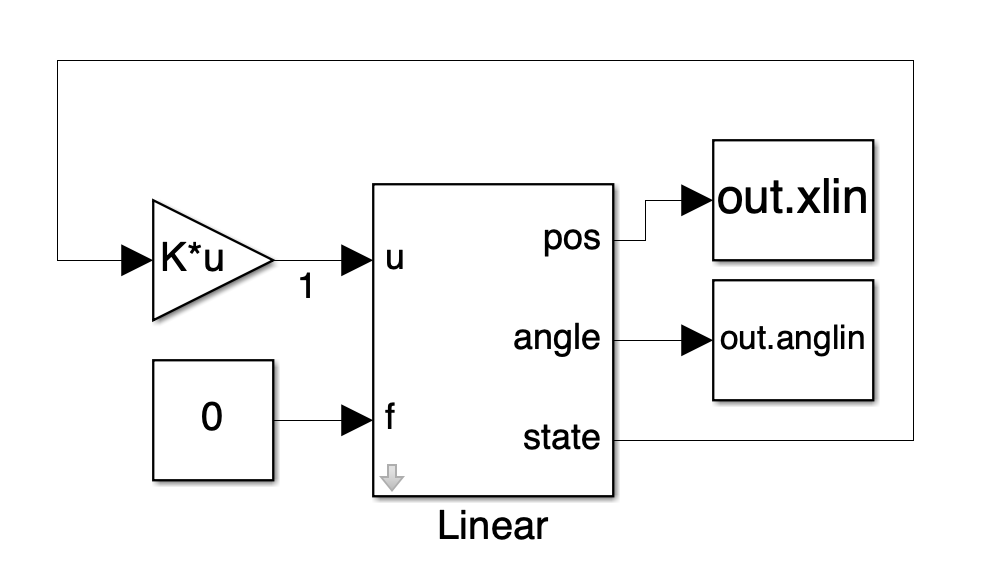
\includegraphics[width=0.7\textwidth]{media/modal_control_linear_scheme.png}
    \caption{Схема моделирования линейной модели системы с модальным регулятором}
    \label{fig:modal_control_scheme_linear}
\end{figure}
\begin{figure}[ht!]
    \centering
    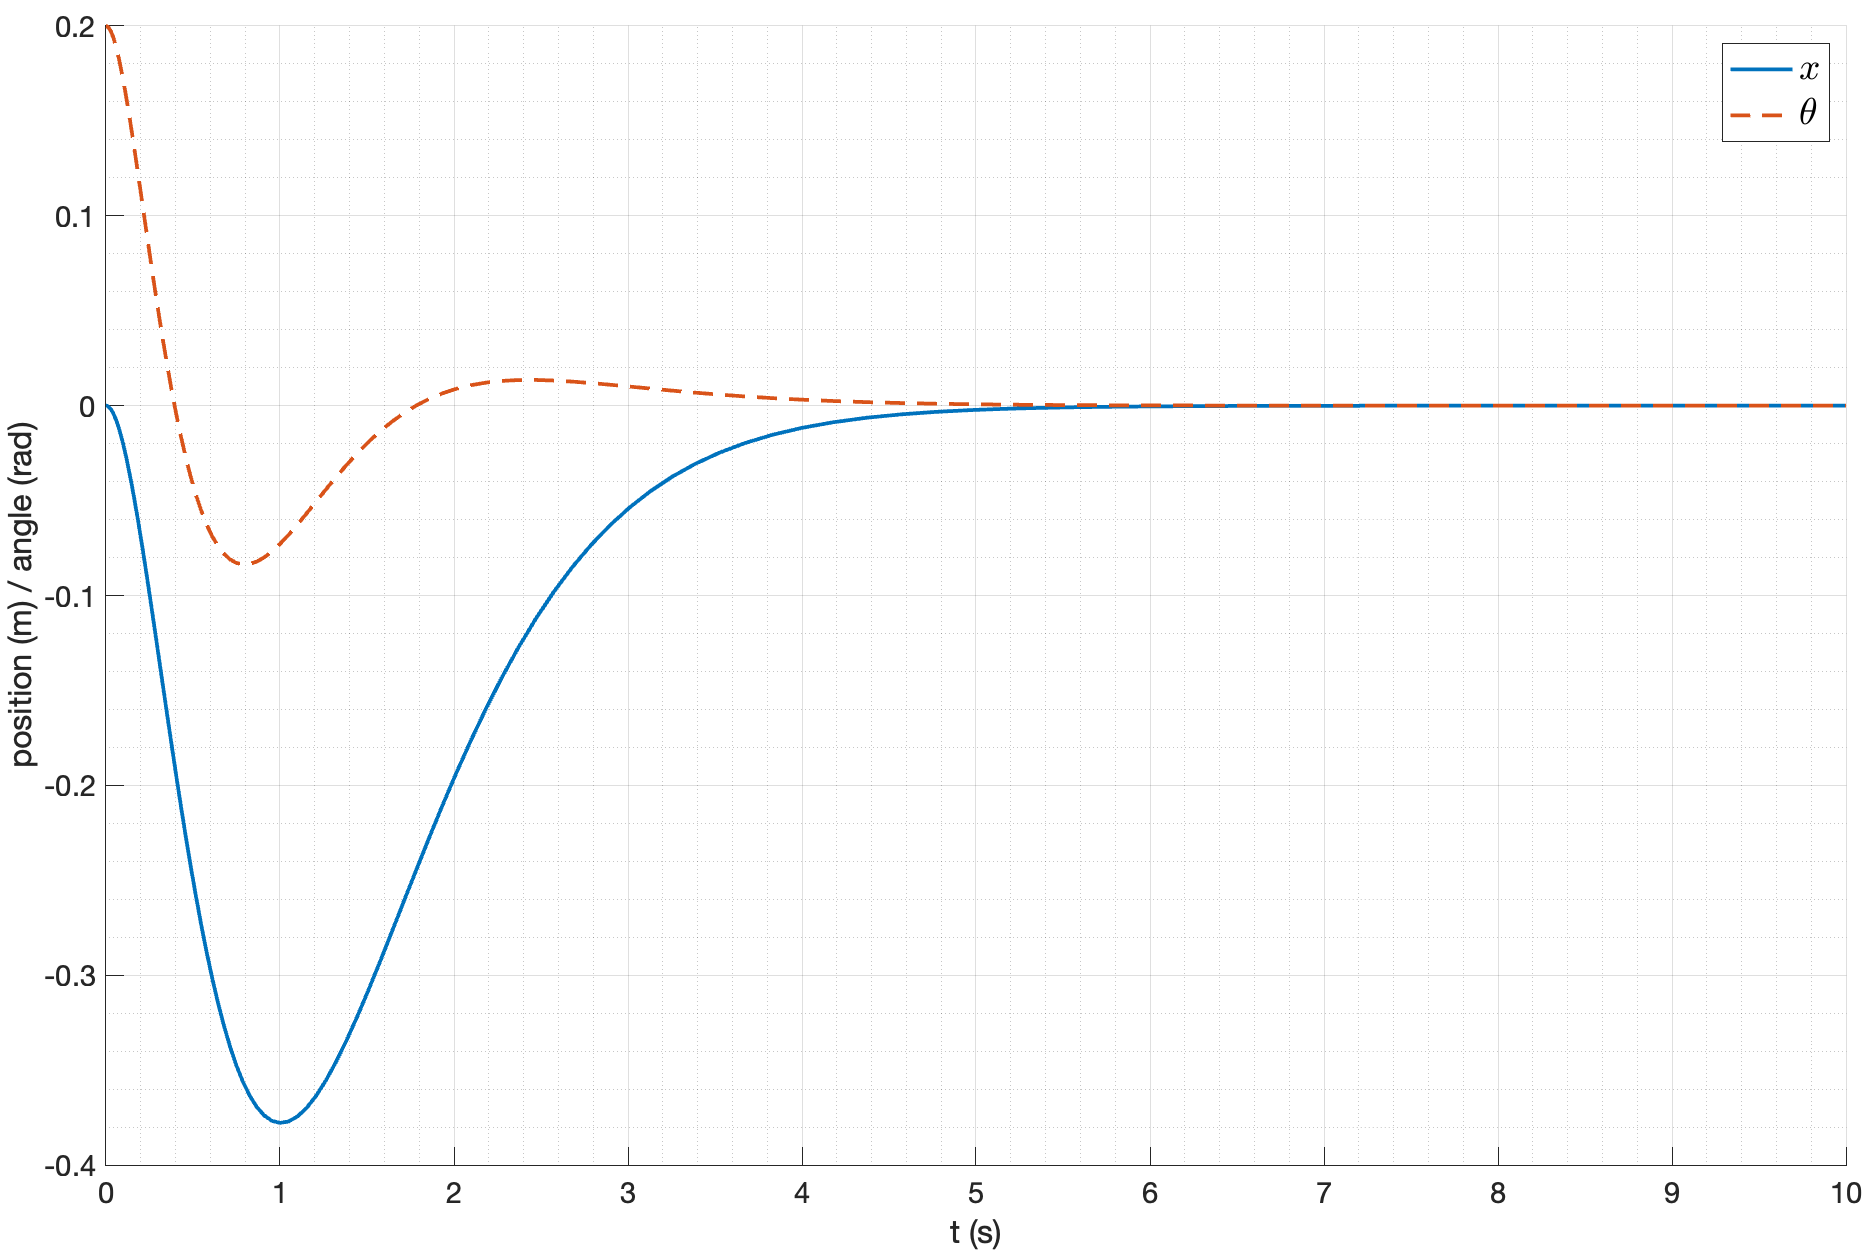
\includegraphics[width=0.8\textwidth]{media/plots/modal_control/modal_control_linear_out_0.png}
    \caption{Результаты моделирования линейной модели системы с модальным регулятором}
    \label{fig:modal_control_linear_out}
\end{figure}

Можно заметить, что приходит в равновесное состояние. Теперь попробуем использовать этот же 
модальный регулятор на нелинейной модели системы. Схема моделирования приведена на
рисунке \ref{fig:modal_control_scheme_nonlinear}. Результаты моделирования приведены на
рисунке \ref{fig:modal_control_nonlinear_out}.


\begin{figure}[ht!]
    \centering
    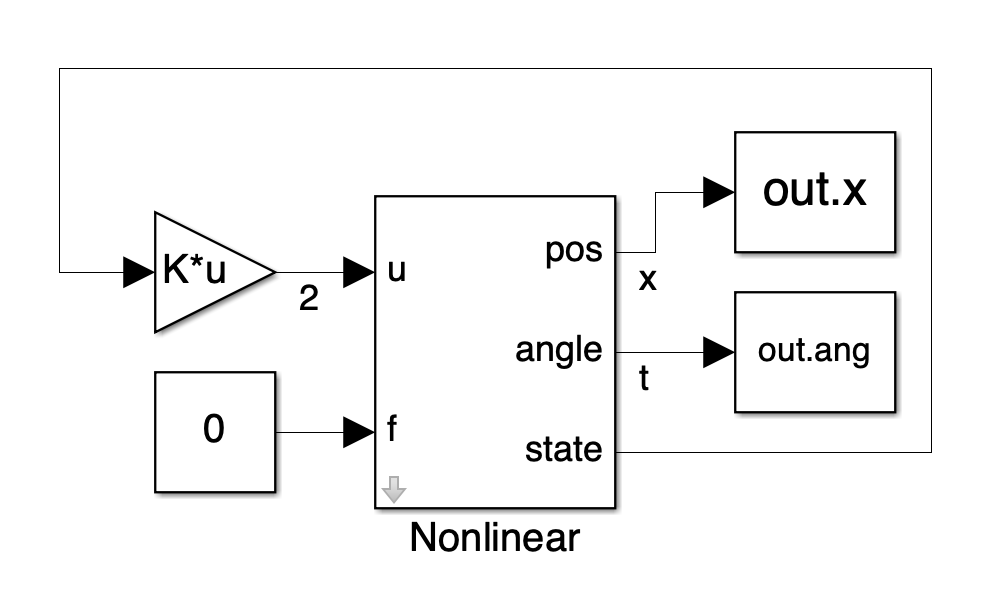
\includegraphics[width=0.7\textwidth]{media/modal_control_scheme.png}
    \caption{Схема моделирования нелинейной модели системы с модальным регулятором}
    \label{fig:modal_control_scheme_nonlinear}
\end{figure}
\begin{figure}[ht!]
    \centering
    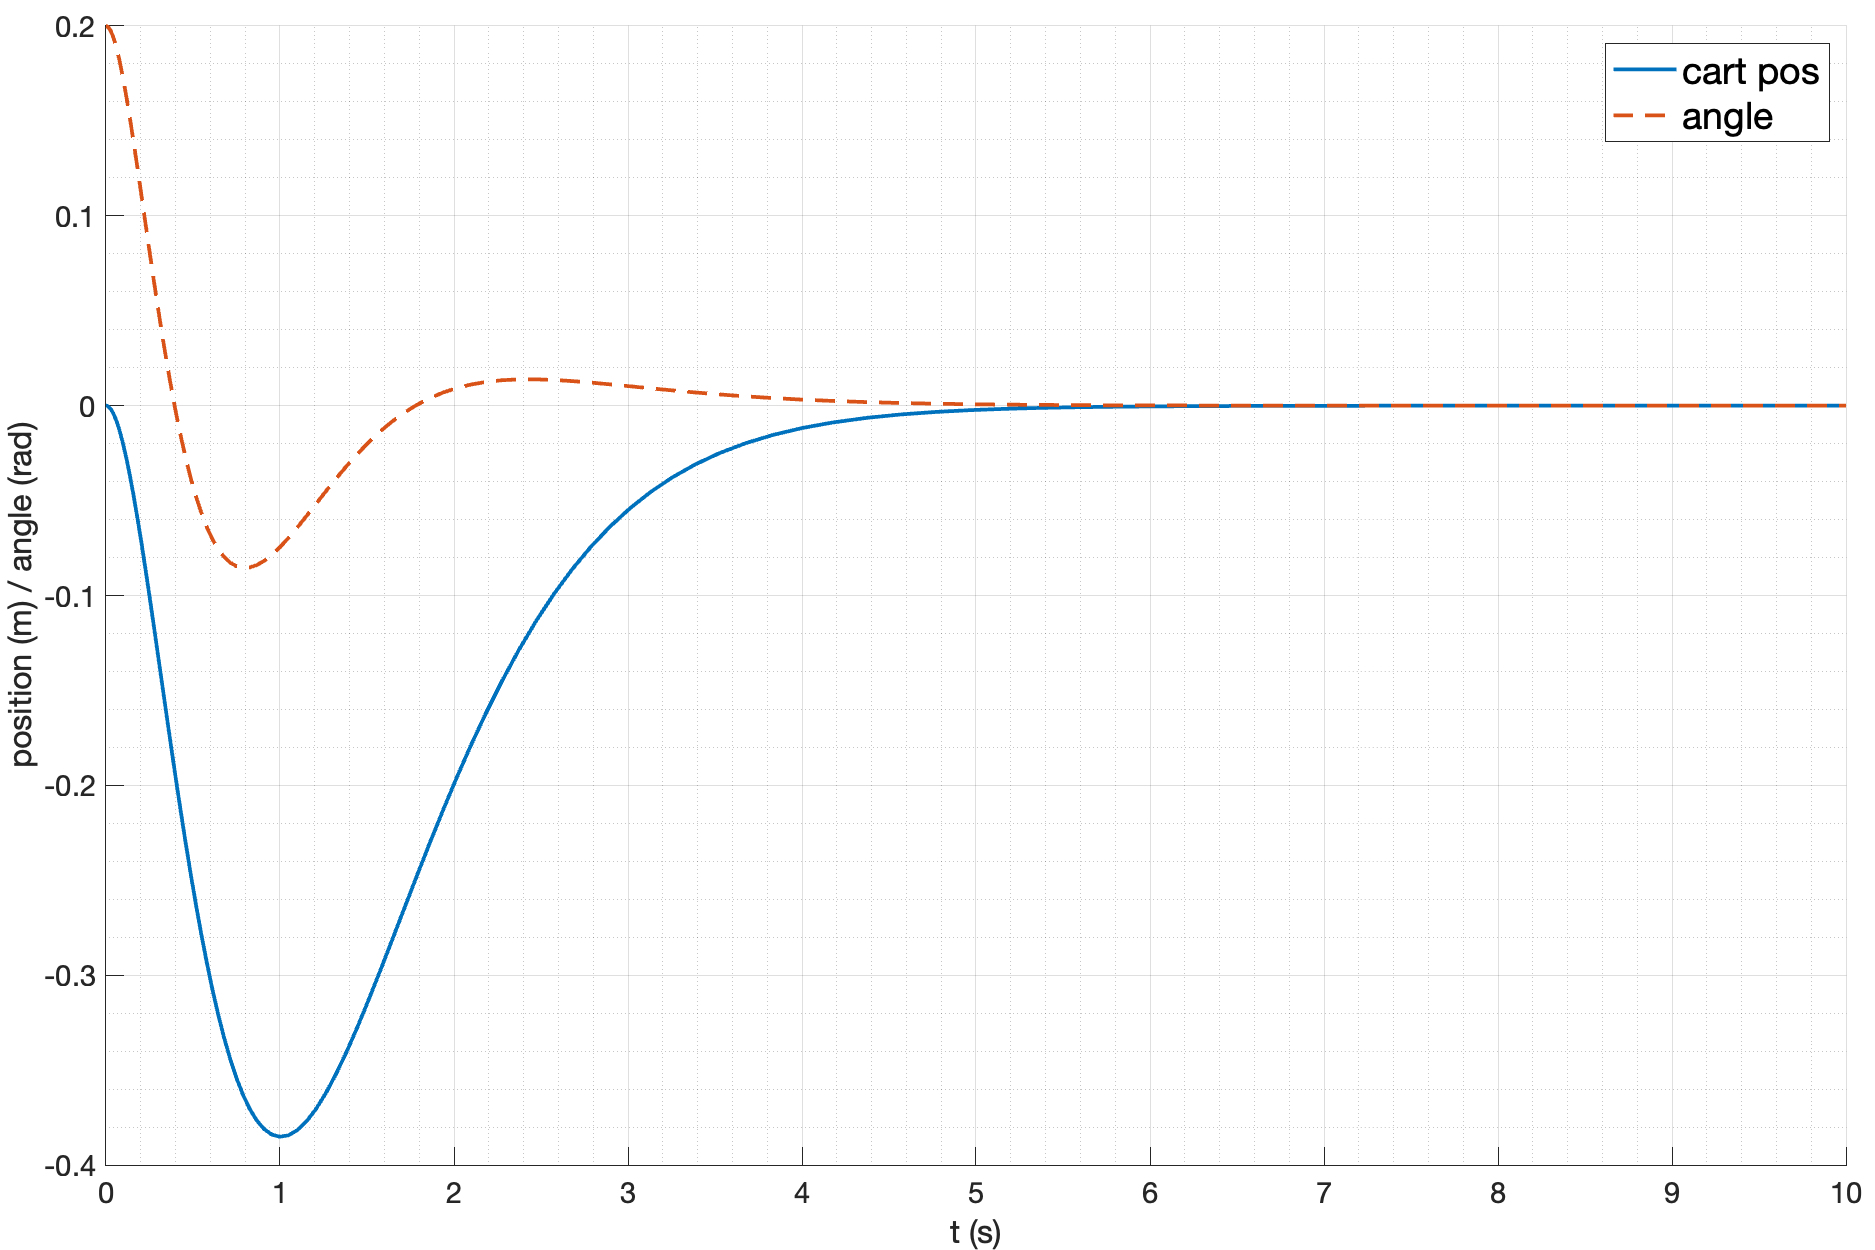
\includegraphics[width=0.8\textwidth]{media/plots/modal_control/modal_control_out_0.png}
    \caption{Результаты моделирования нелинейной модели системы с модальным регулятором}
    \label{fig:modal_control_nonlinear_out}
\end{figure}

Рассмотрим различия между движением линейной и нелинейной модели системы. График различий в движении
представлен на рисунке \ref{fig:modal_control_cmp}.
\begin{figure}[ht!]
    \centering
    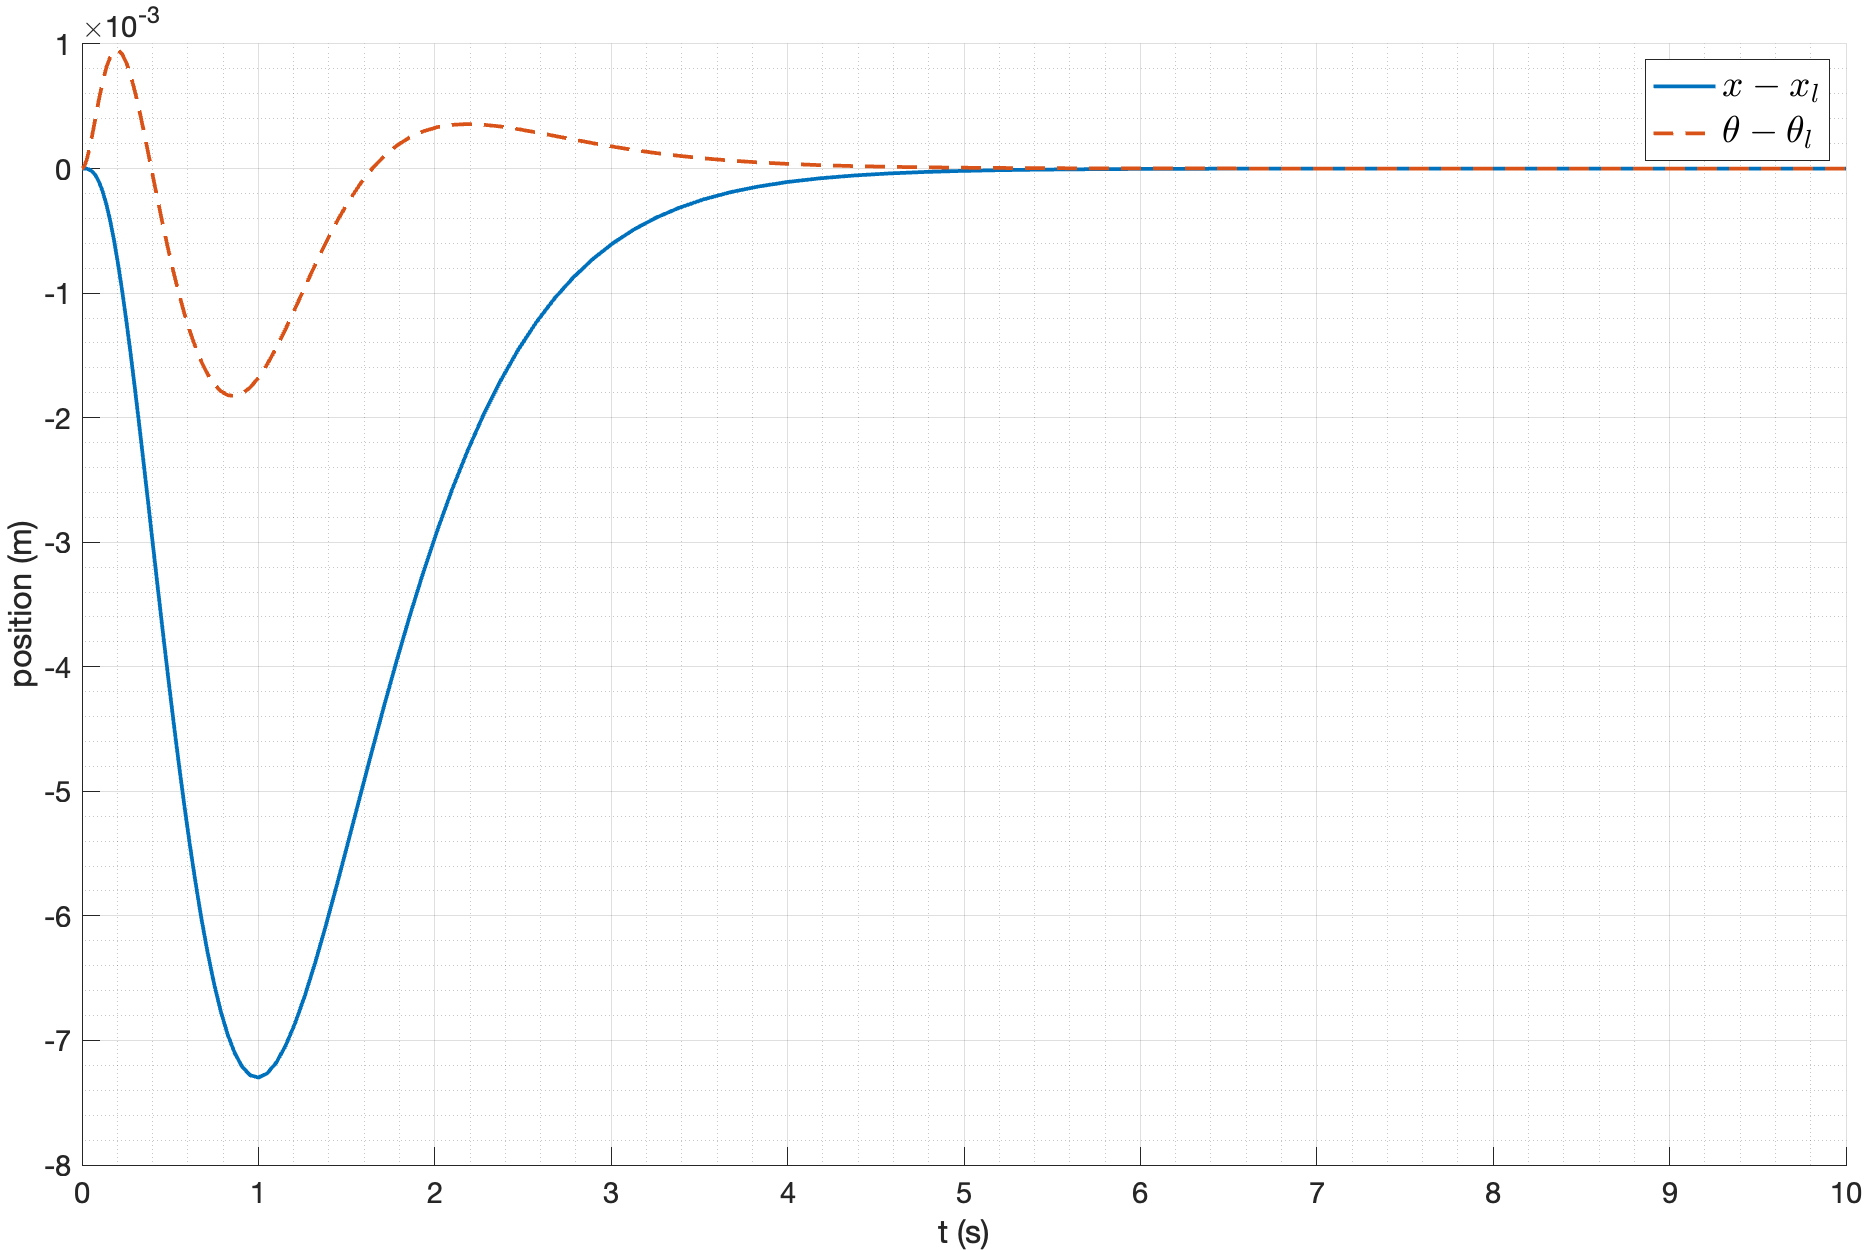
\includegraphics[width=0.8\textwidth]{media/plots/modal_control/modal_control_cmp_0.png}
    \caption{Различия в движении линейной и нелинейной модели системы с модальным регулятором}
    \label{fig:modal_control_cmp}
\end{figure}
Видно, что различие между углом отклонения маятника не превышает $10^{-3}$ радиан, а различие между
координатами тележки не превышает $8\cdot10^{-3}$ метра. Данный результат можно считать удовлетворительным, 
регулятор, синтезированный для линейной модели системы, обеспечивает приемлемое качество управления 
нелинейной модели системы. 

\FloatBarrier
\subsection{Исследование устойчивости при различных начальных условиях}
Проверим работу данного регулятора при различных начальных условиях. 
В качестве начальных условий возьмем различные начальные углы отклонения маятника $\theta_0 \in \begin{bmatrix}0.3, 0.7, 0.9, 1.0, 1.1, 1.2\end{bmatrix}$. Результаты 
моделирования приведены на рисунке \ref{fig:modal_control_initials}. 
\begin{figure}[ht!]
    \centering
    \begin{subfigure}[b]{0.45\textwidth}
        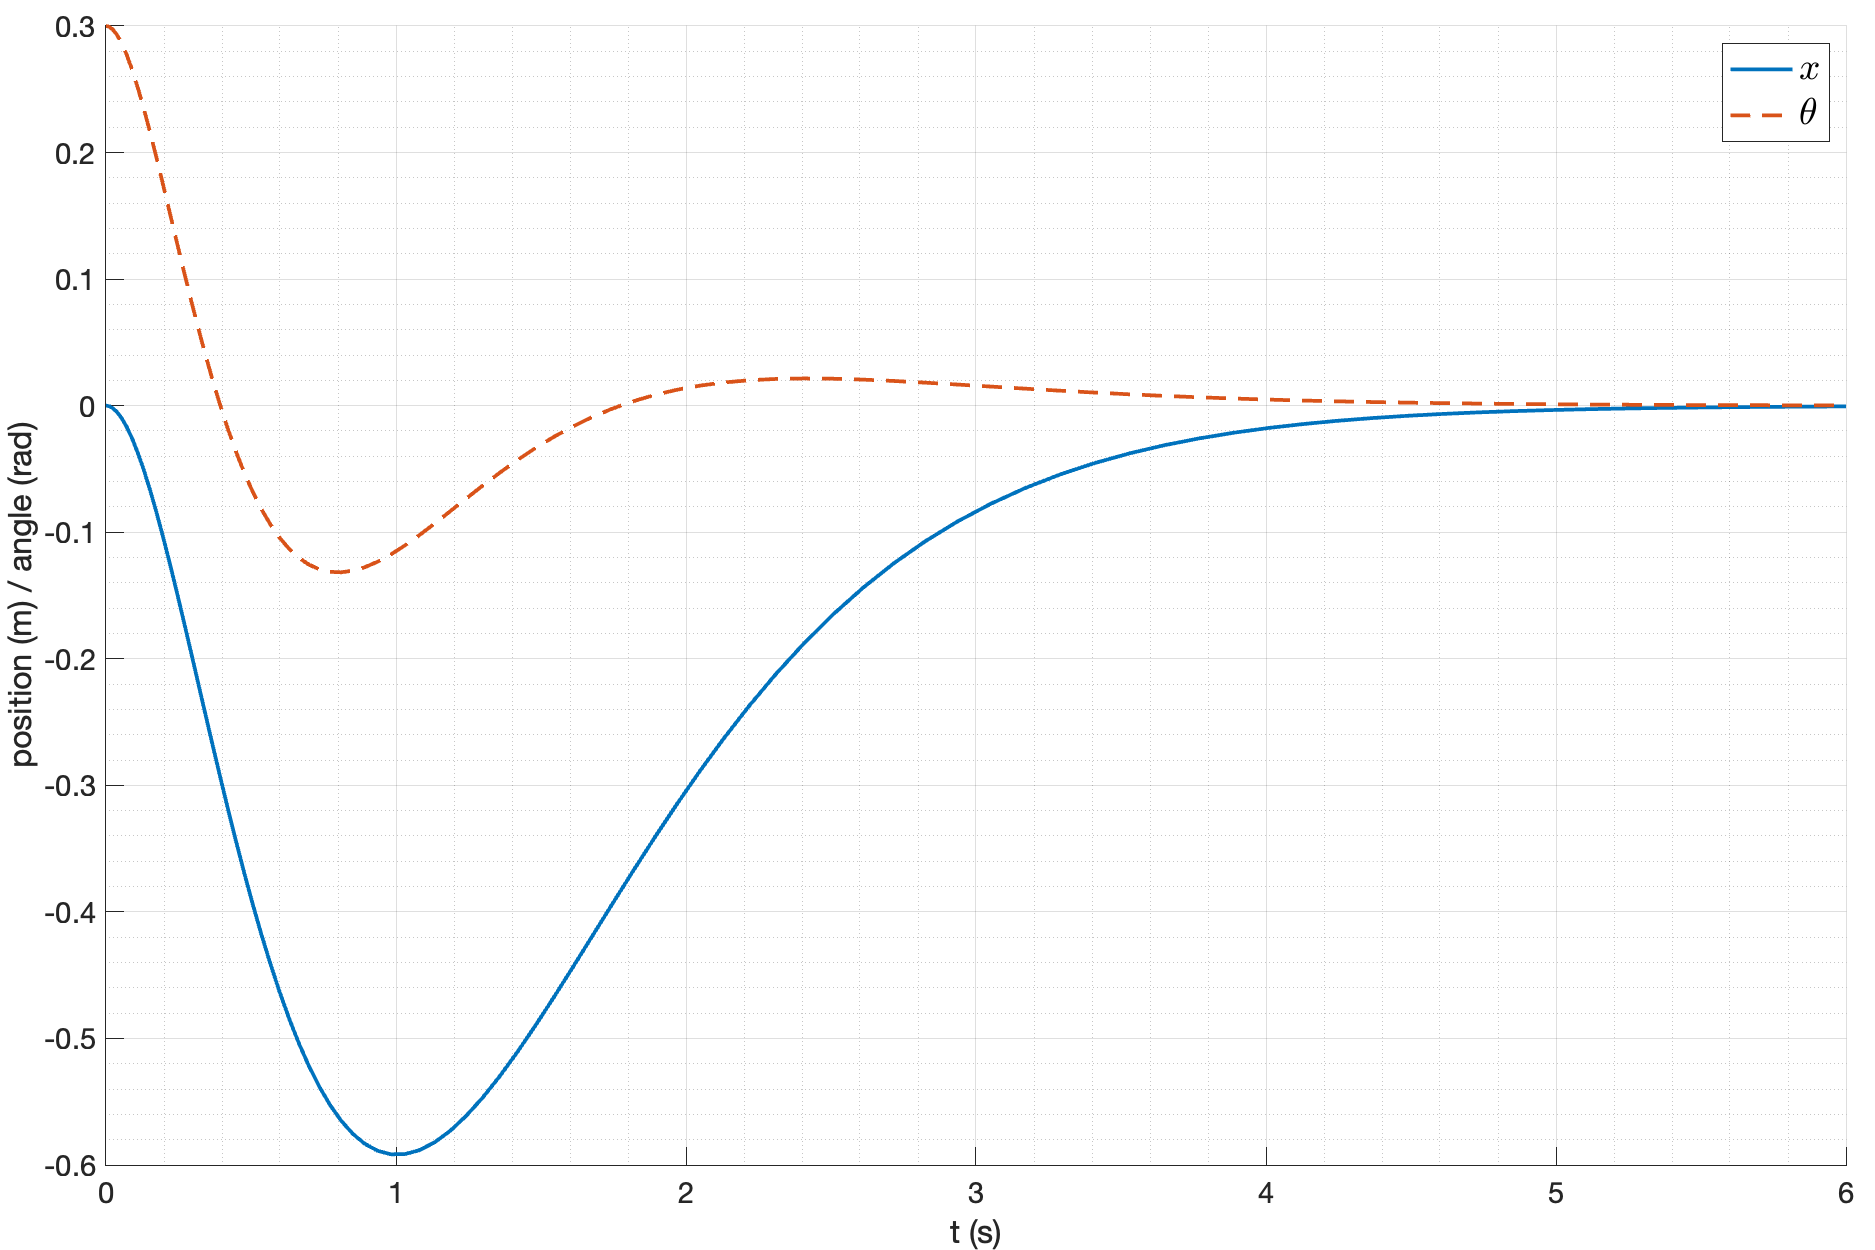
\includegraphics[width=\textwidth]{media/plots/modal_control/modal_control_out_1.png}
        \caption{$\theta_0 = 0.3$}
    \end{subfigure}
    \begin{subfigure}[b]{0.45\textwidth}
        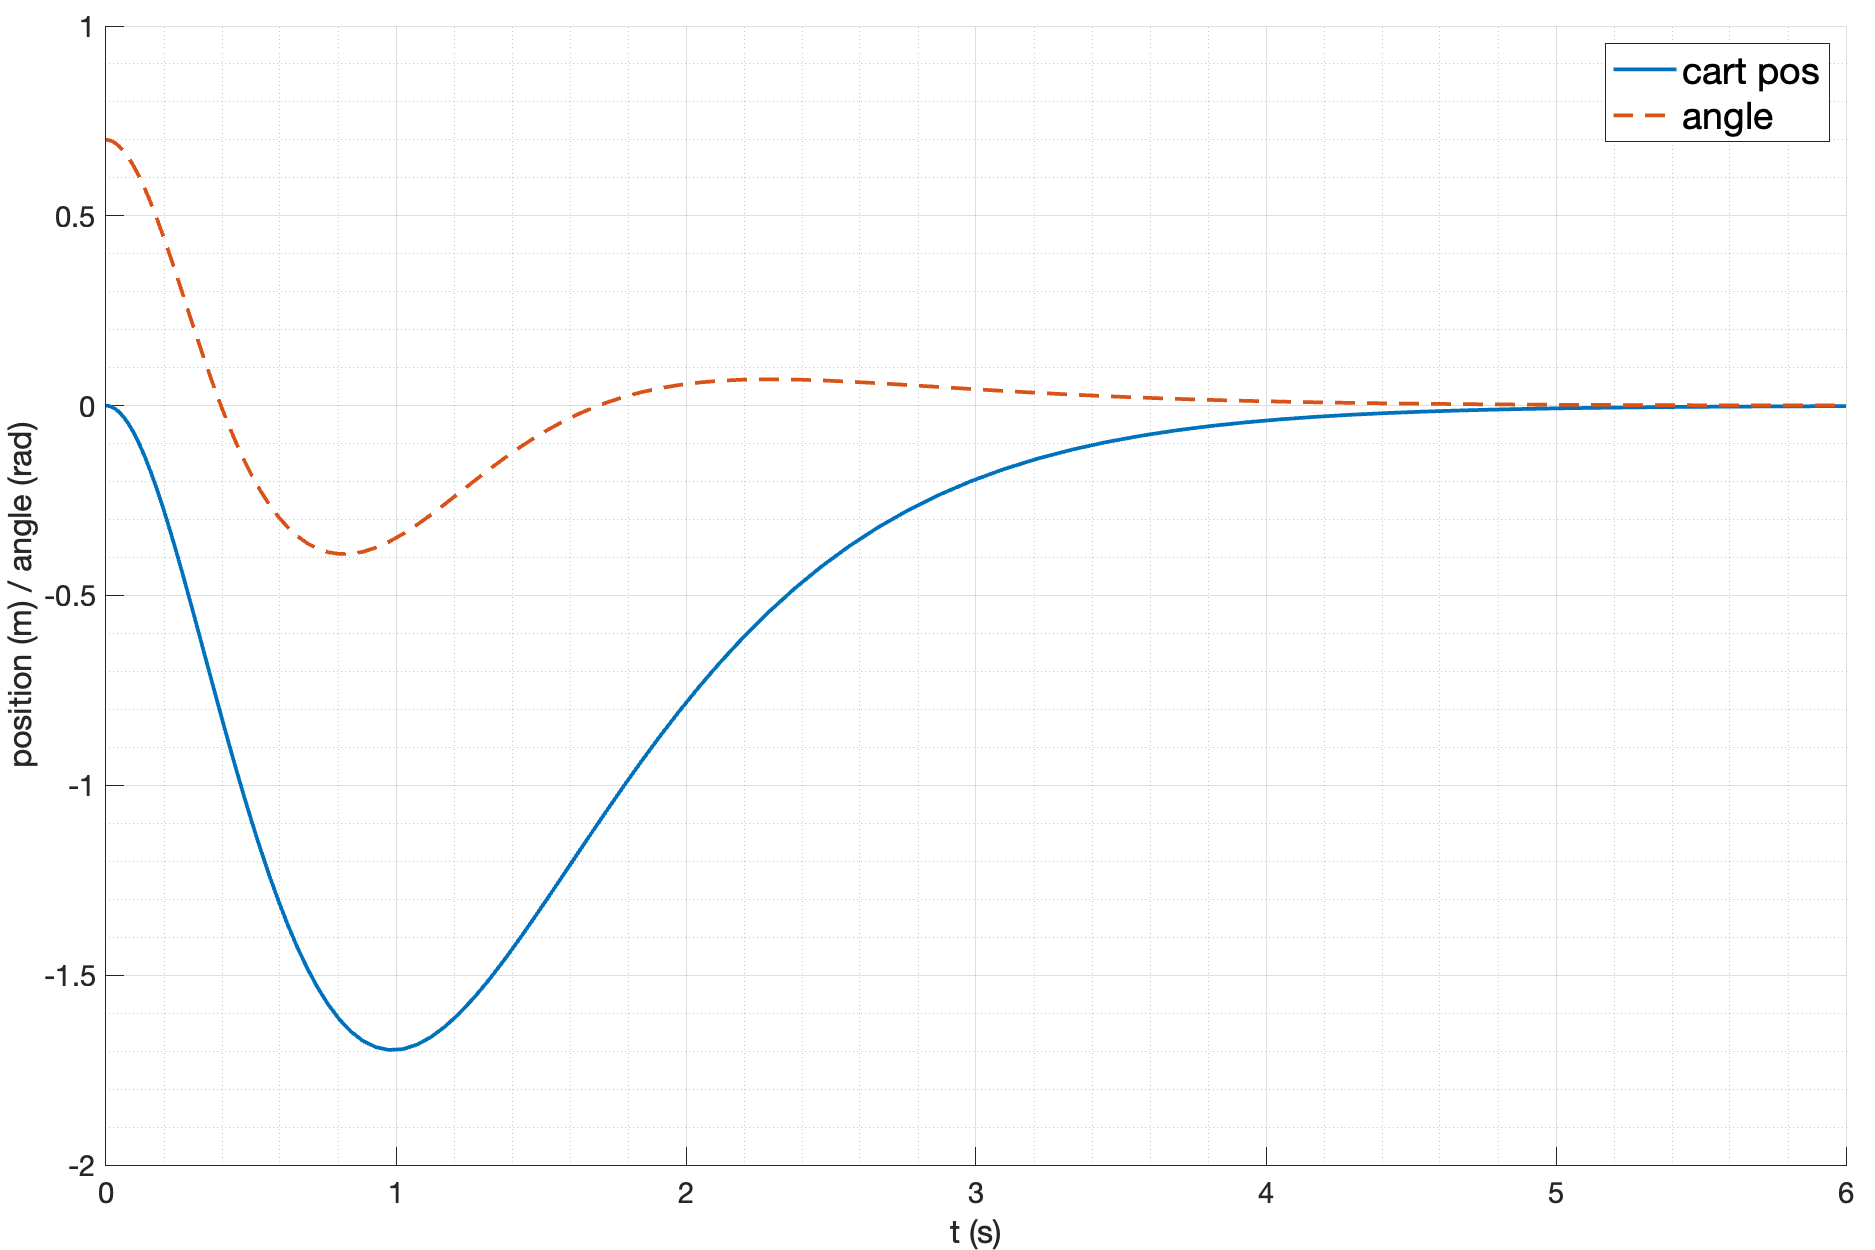
\includegraphics[width=\textwidth]{media/plots/modal_control/modal_control_out_2.png}
        \caption{$\theta_0 = 0.7$}
    \end{subfigure}
    \begin{subfigure}[b]{0.45\textwidth}
        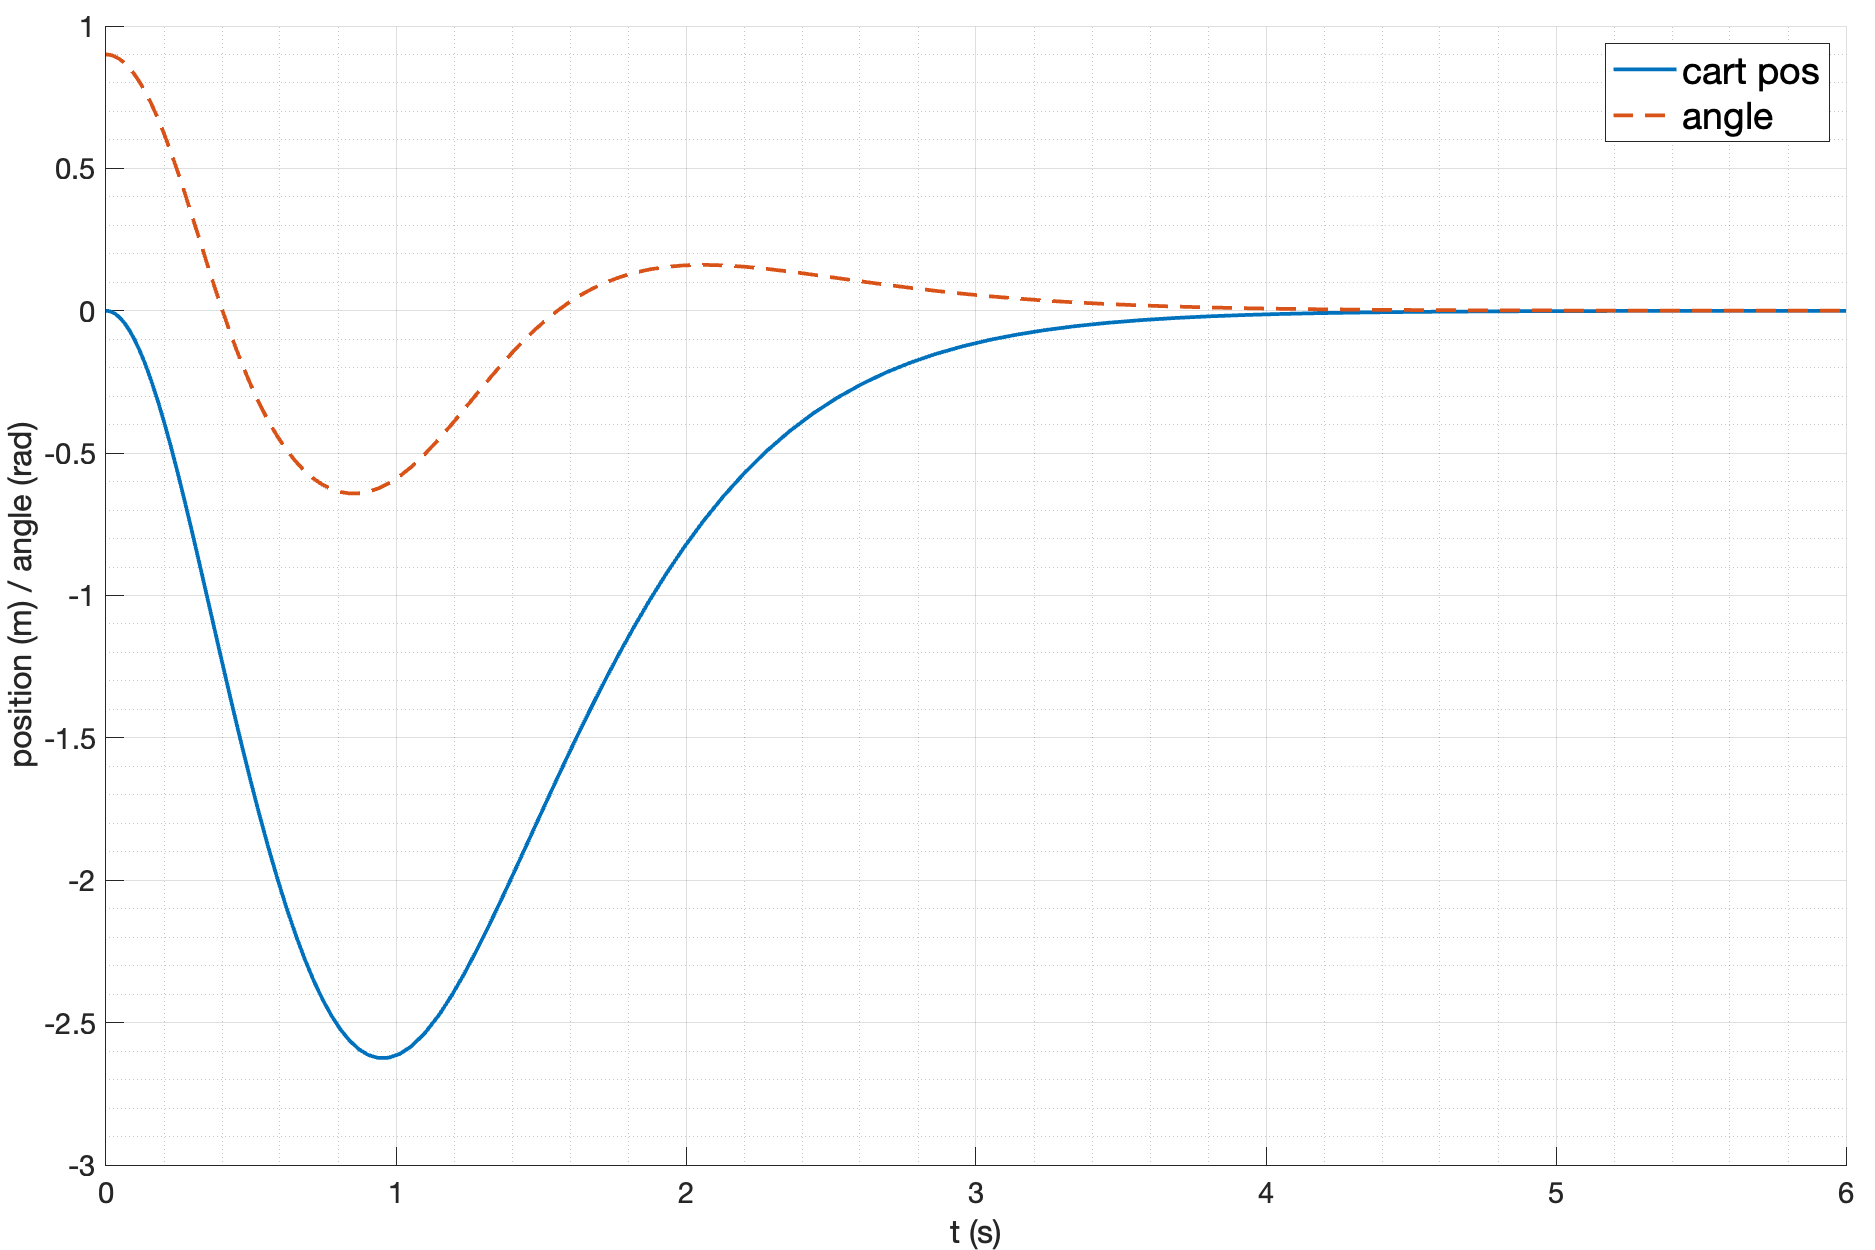
\includegraphics[width=\textwidth]{media/plots/modal_control/modal_control_out_3.png}
        \caption{$\theta_0 = 0.9$}
    \end{subfigure}
    \begin{subfigure}[b]{0.45\textwidth}
        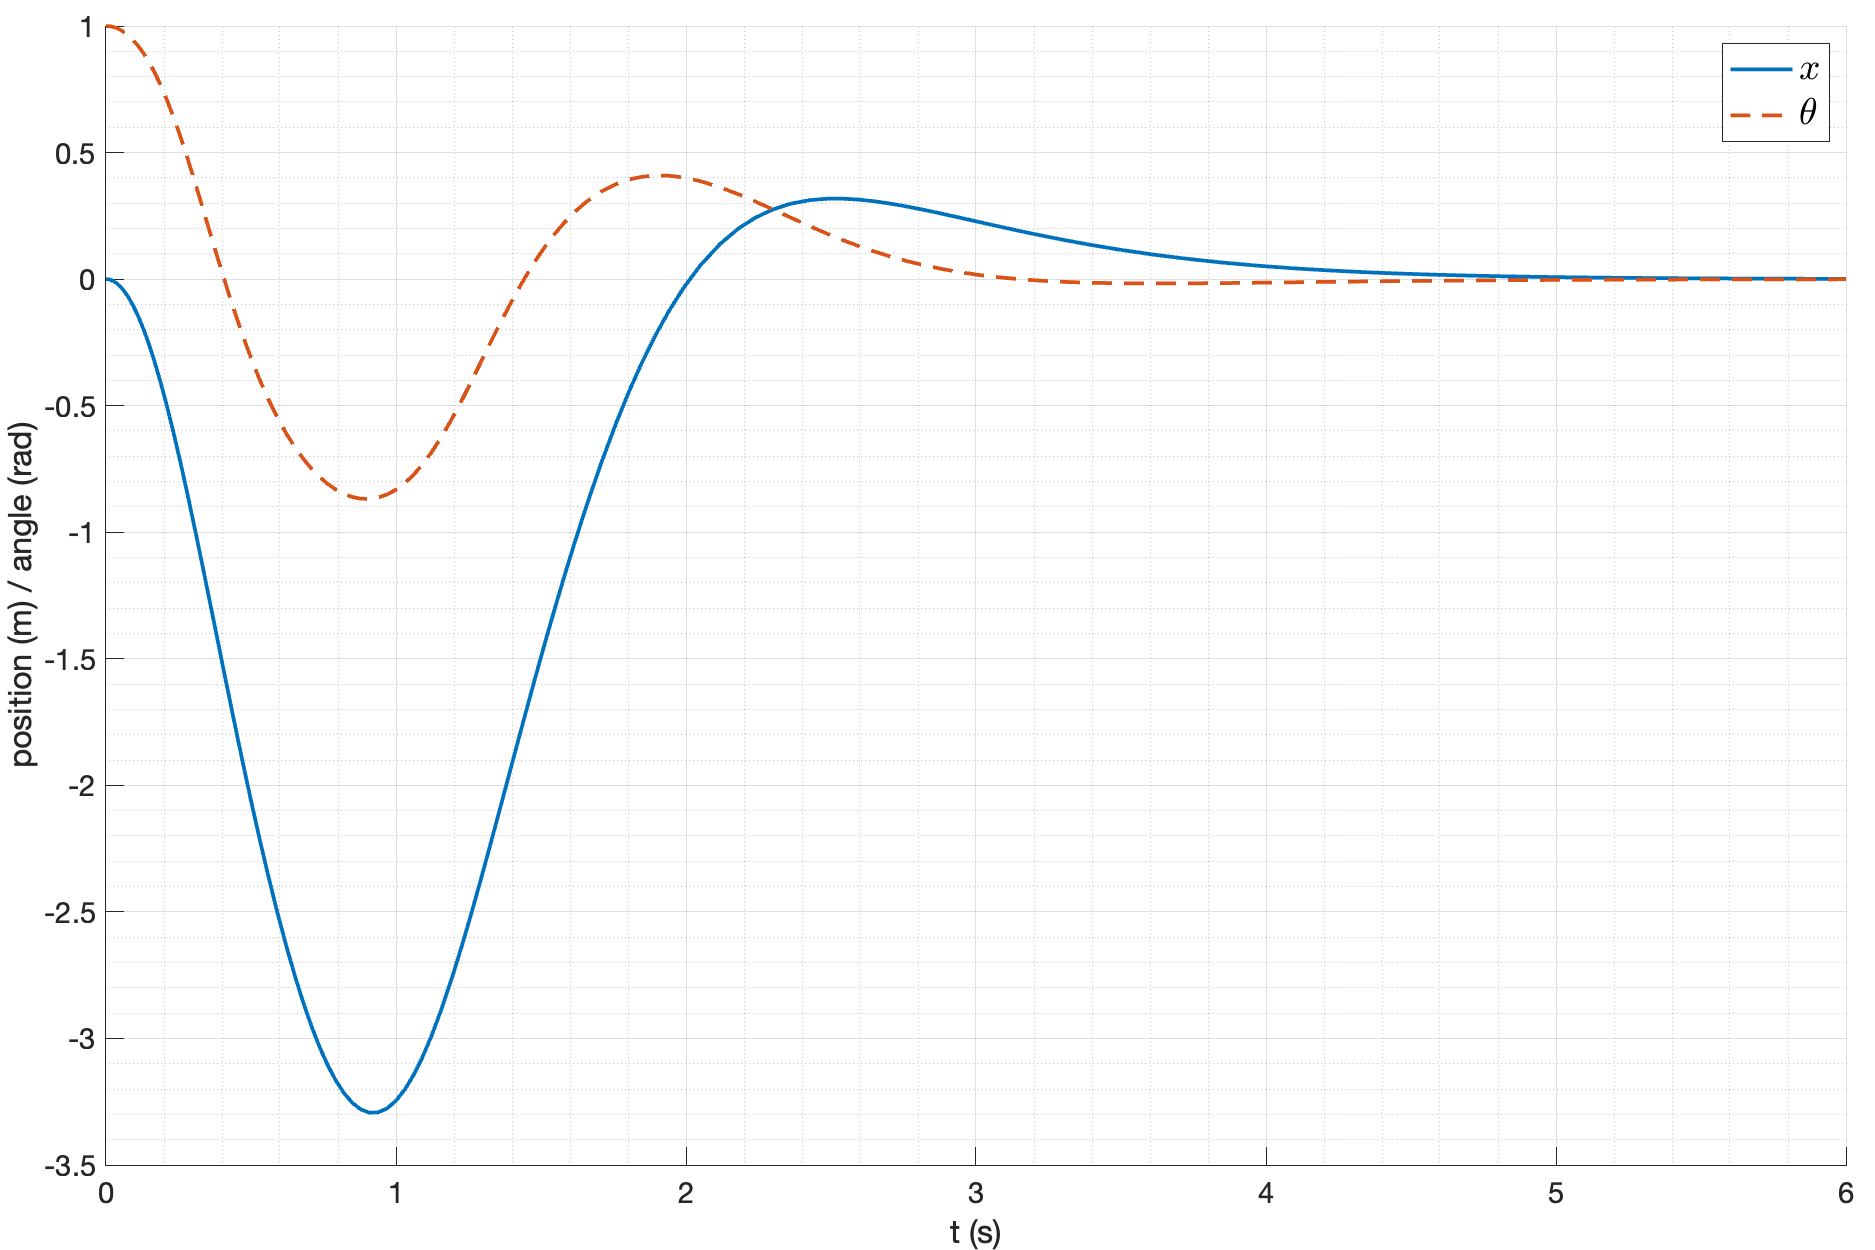
\includegraphics[width=\textwidth]{media/plots/modal_control/modal_control_out_4.png}
        \caption{$\theta_0 = 1.0$}
    \end{subfigure}
    \begin{subfigure}[b]{0.45\textwidth}
        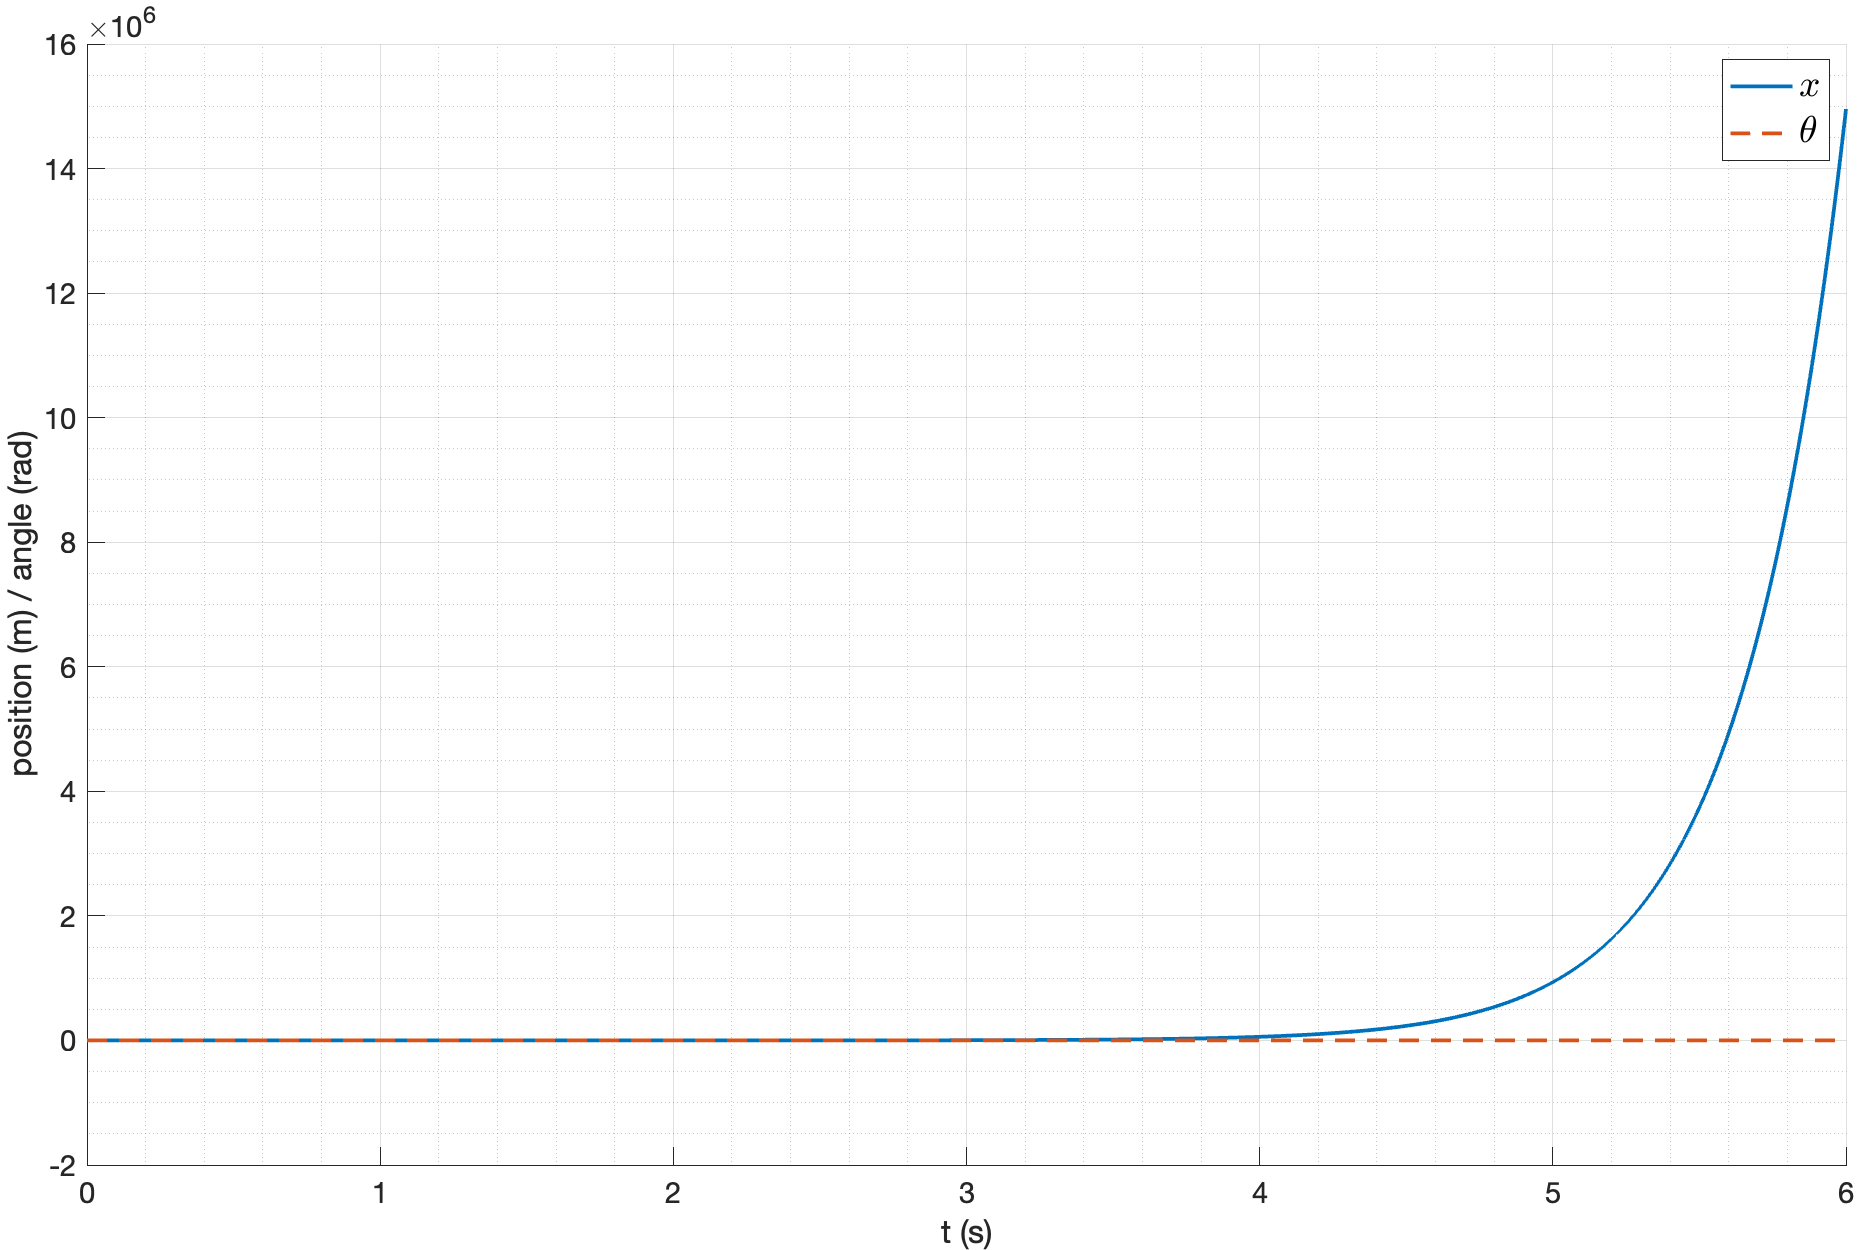
\includegraphics[width=\textwidth]{media/plots/modal_control/modal_control_out_5.png}
        \caption{$\theta_0 = 1.1$}
    \end{subfigure}
    \begin{subfigure}[b]{0.45\textwidth}
        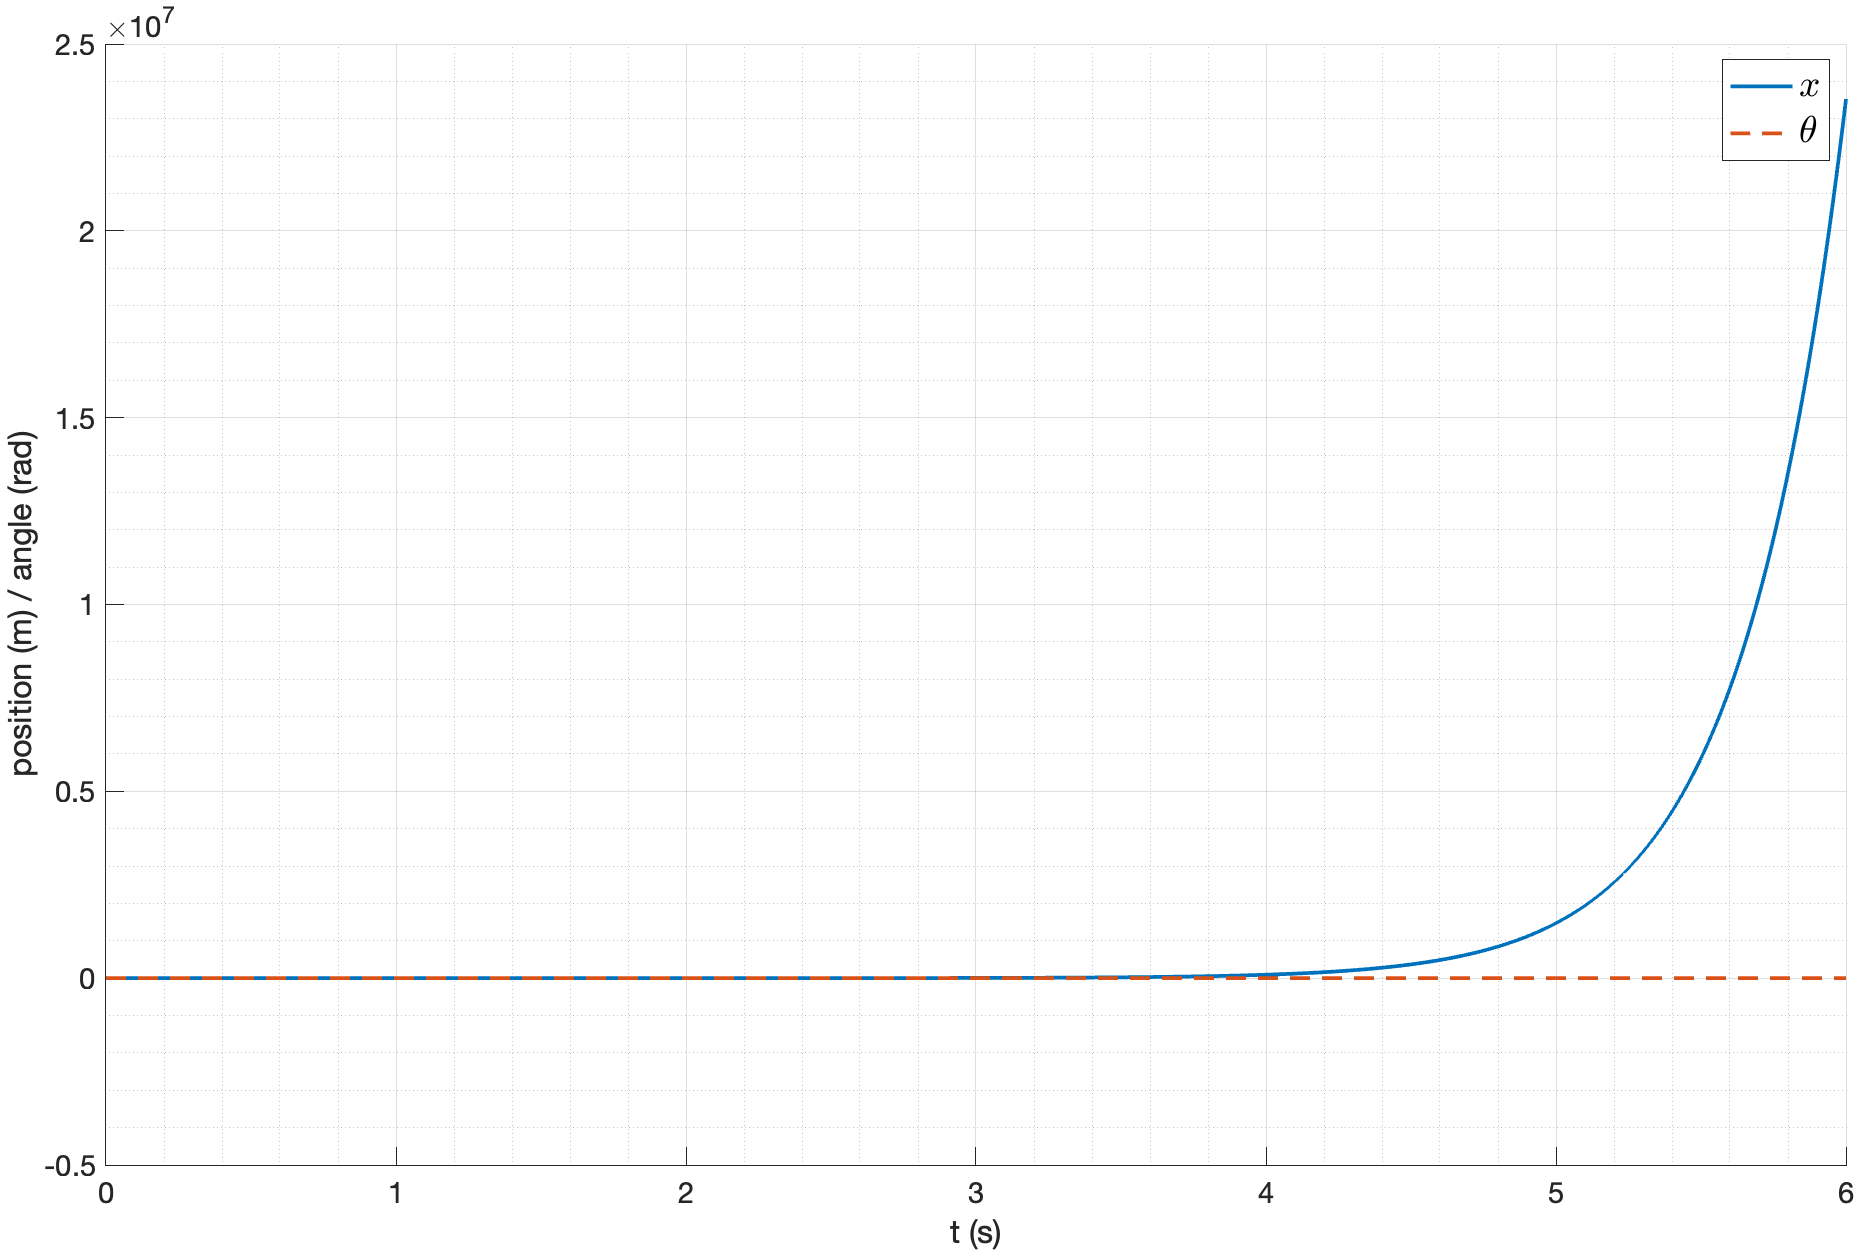
\includegraphics[width=\textwidth]{media/plots/modal_control/modal_control_out_6.png}
        \caption{$\theta_0 = 1.2$}
    \end{subfigure}
    \caption{Модальное управление нелинейной модели системы}
    \label{fig:modal_control_initials}
\end{figure}
Видно, что при начальном угле отклонения маятника вплоть до $\theta_0 = 1.0$ система приходит в
равновесное состояние. При этом время переходного процесса остается приблизительно одинаковым. 
При дальнейшем увеличении угла начального отклонения маятника система не приходит в равновесное состояние, 
это связано с тем, что при больших отклонениях маятника от вертикального положения линейная модель, на основе 
которой был синтезирован регулятор, перестает адекватно описывать поведение системы. Убедиться в этом можно 
посмотрев на график поведения линейной модели системы при начальном угле отклонения $\theta_0 = 1.2$ (рисунок \ref{fig:modal_control_linear_out_6}).
\begin{figure}[ht!]
    \centering
    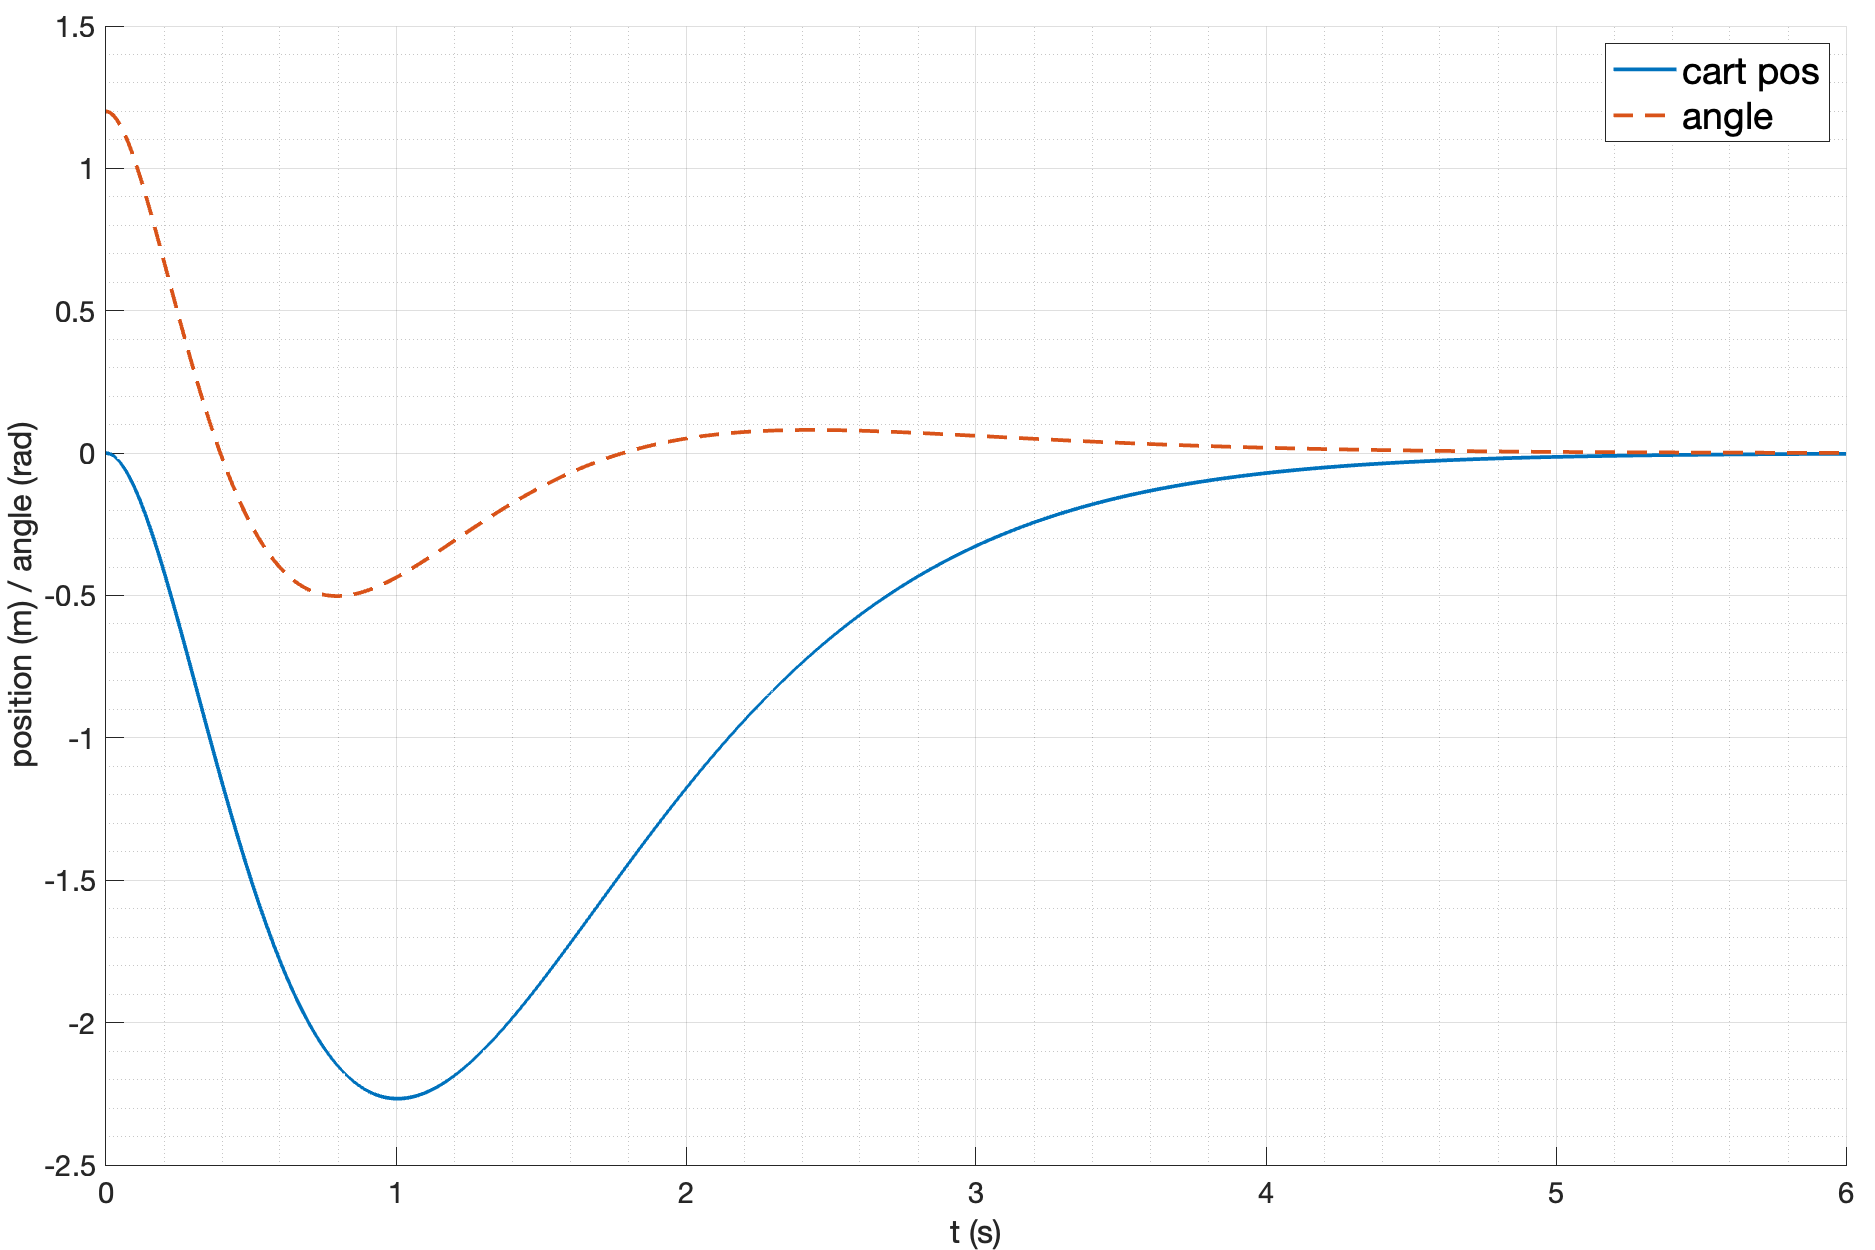
\includegraphics[width=\textwidth]{media/plots/modal_control/modal_control_linear_out_6.png}
    \caption{Результаты моделирования линейной модели системы с модальным регулятором при $\theta_0 = 1.2$}
    \label{fig:modal_control_linear_out_6}
\end{figure}
Видно, что линейная модель система приходит в равновесное состояния, в отличие от нелинейной модели.

\subsection{Исследование переходного процесса}
Будем рассматривать переходный процесс и управляющее воздействие при различных собственных числах замкнутой регулятором системы. 
В качестве начальных условий возьмем $\theta_0 = 0.3$. Для начала, рассмотрим регуляторы, обеспечивающие спектр 
замкнутой системы вида $\sigma_k = \begin{bmatrix}k & k & k & k\end{bmatrix}$, где $k \in \begin{bmatrix}-4, -6, -8, -10\end{bmatrix}$. 
Результаты моделирования приведены на рисунках \ref{fig:modal_controlers_1_out} -- \ref{fig:modal_controlers_4_u}.

\begin{figure}[ht!]
    \centering
    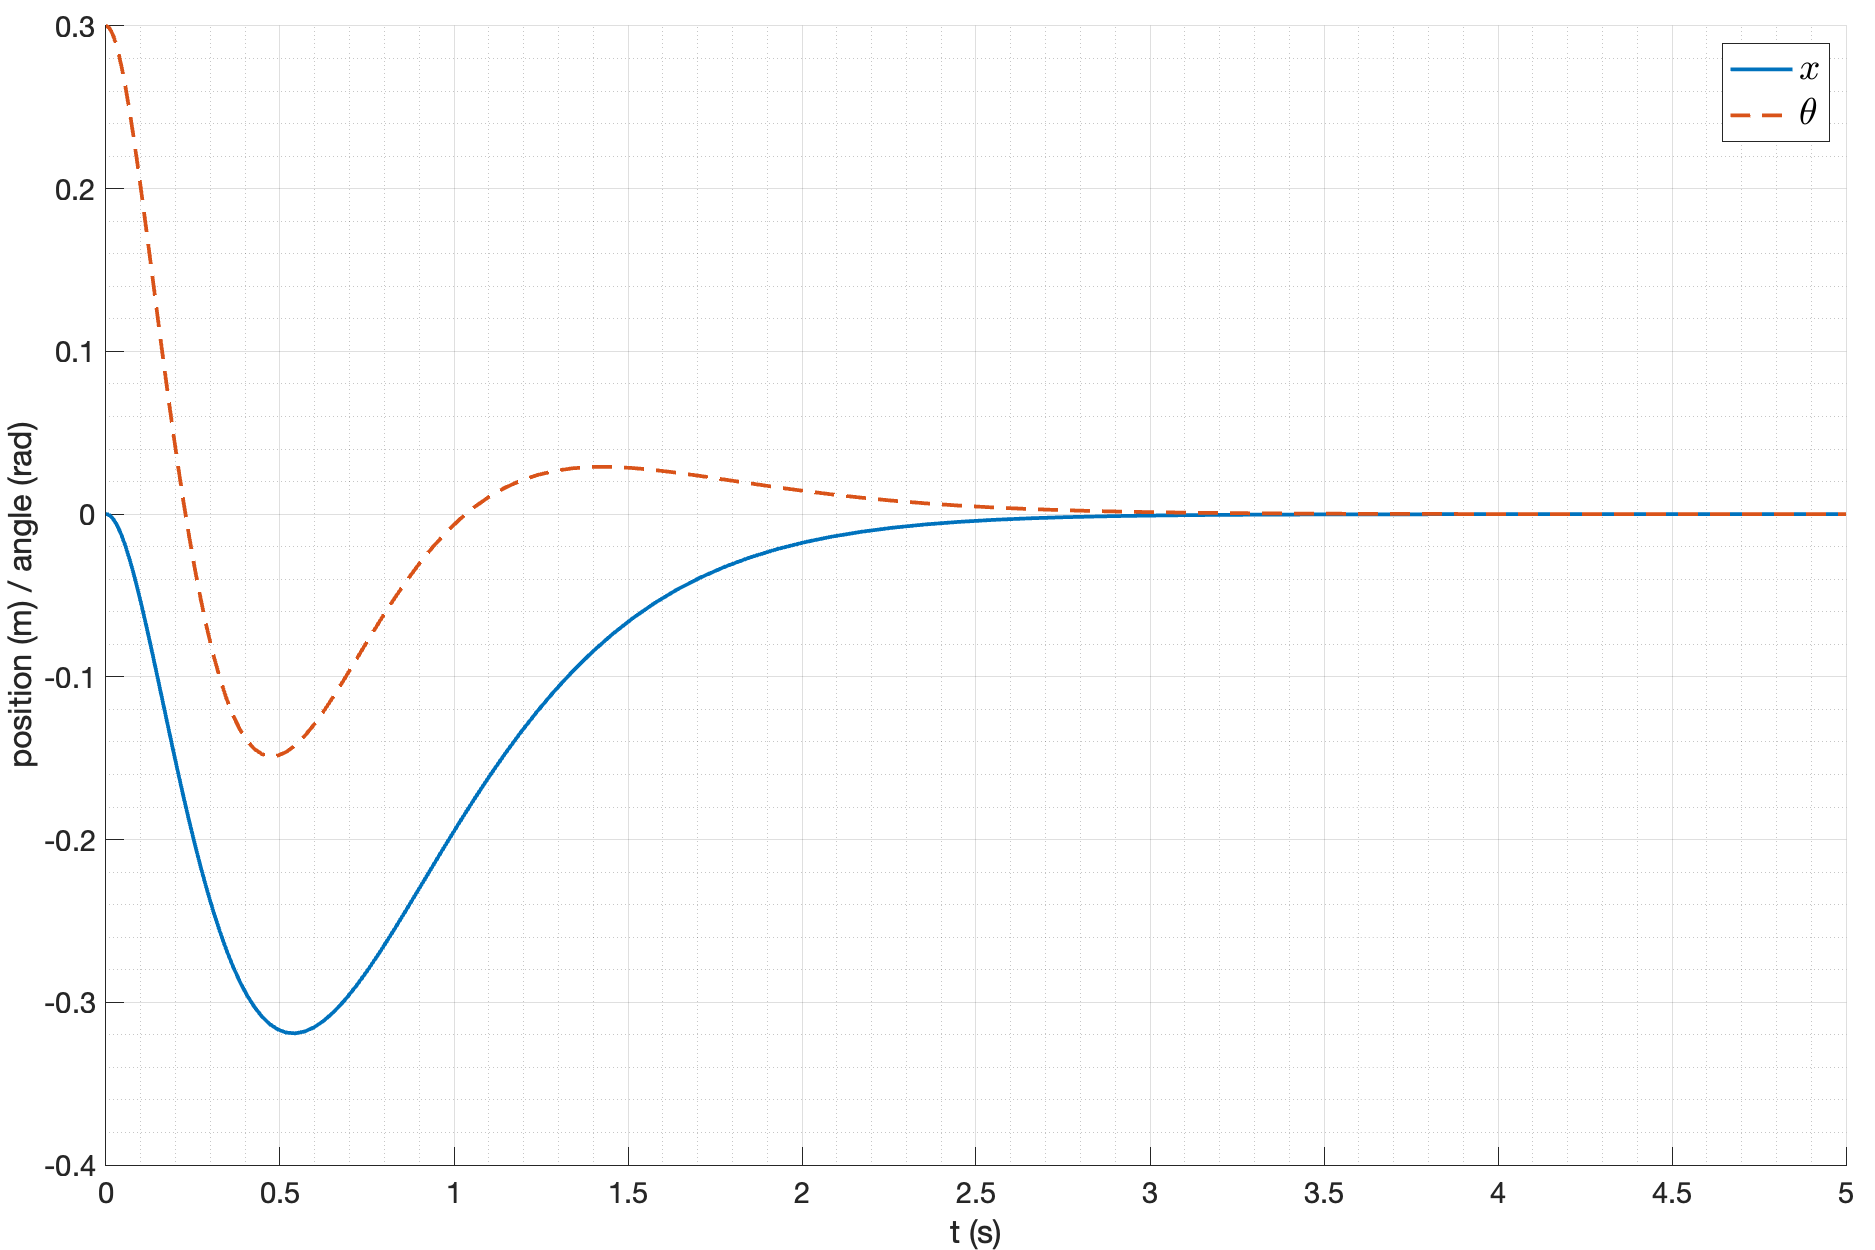
\includegraphics[width=0.8\textwidth]{media/plots/modal_controllers/modal_control_out_1.png}
    \caption{Результаты моделирования нелинейной модели системы с модальным регулятором при $k = -4$}
    \label{fig:modal_controlers_1_out}
\end{figure}
\begin{figure}[ht!]
    \centering
    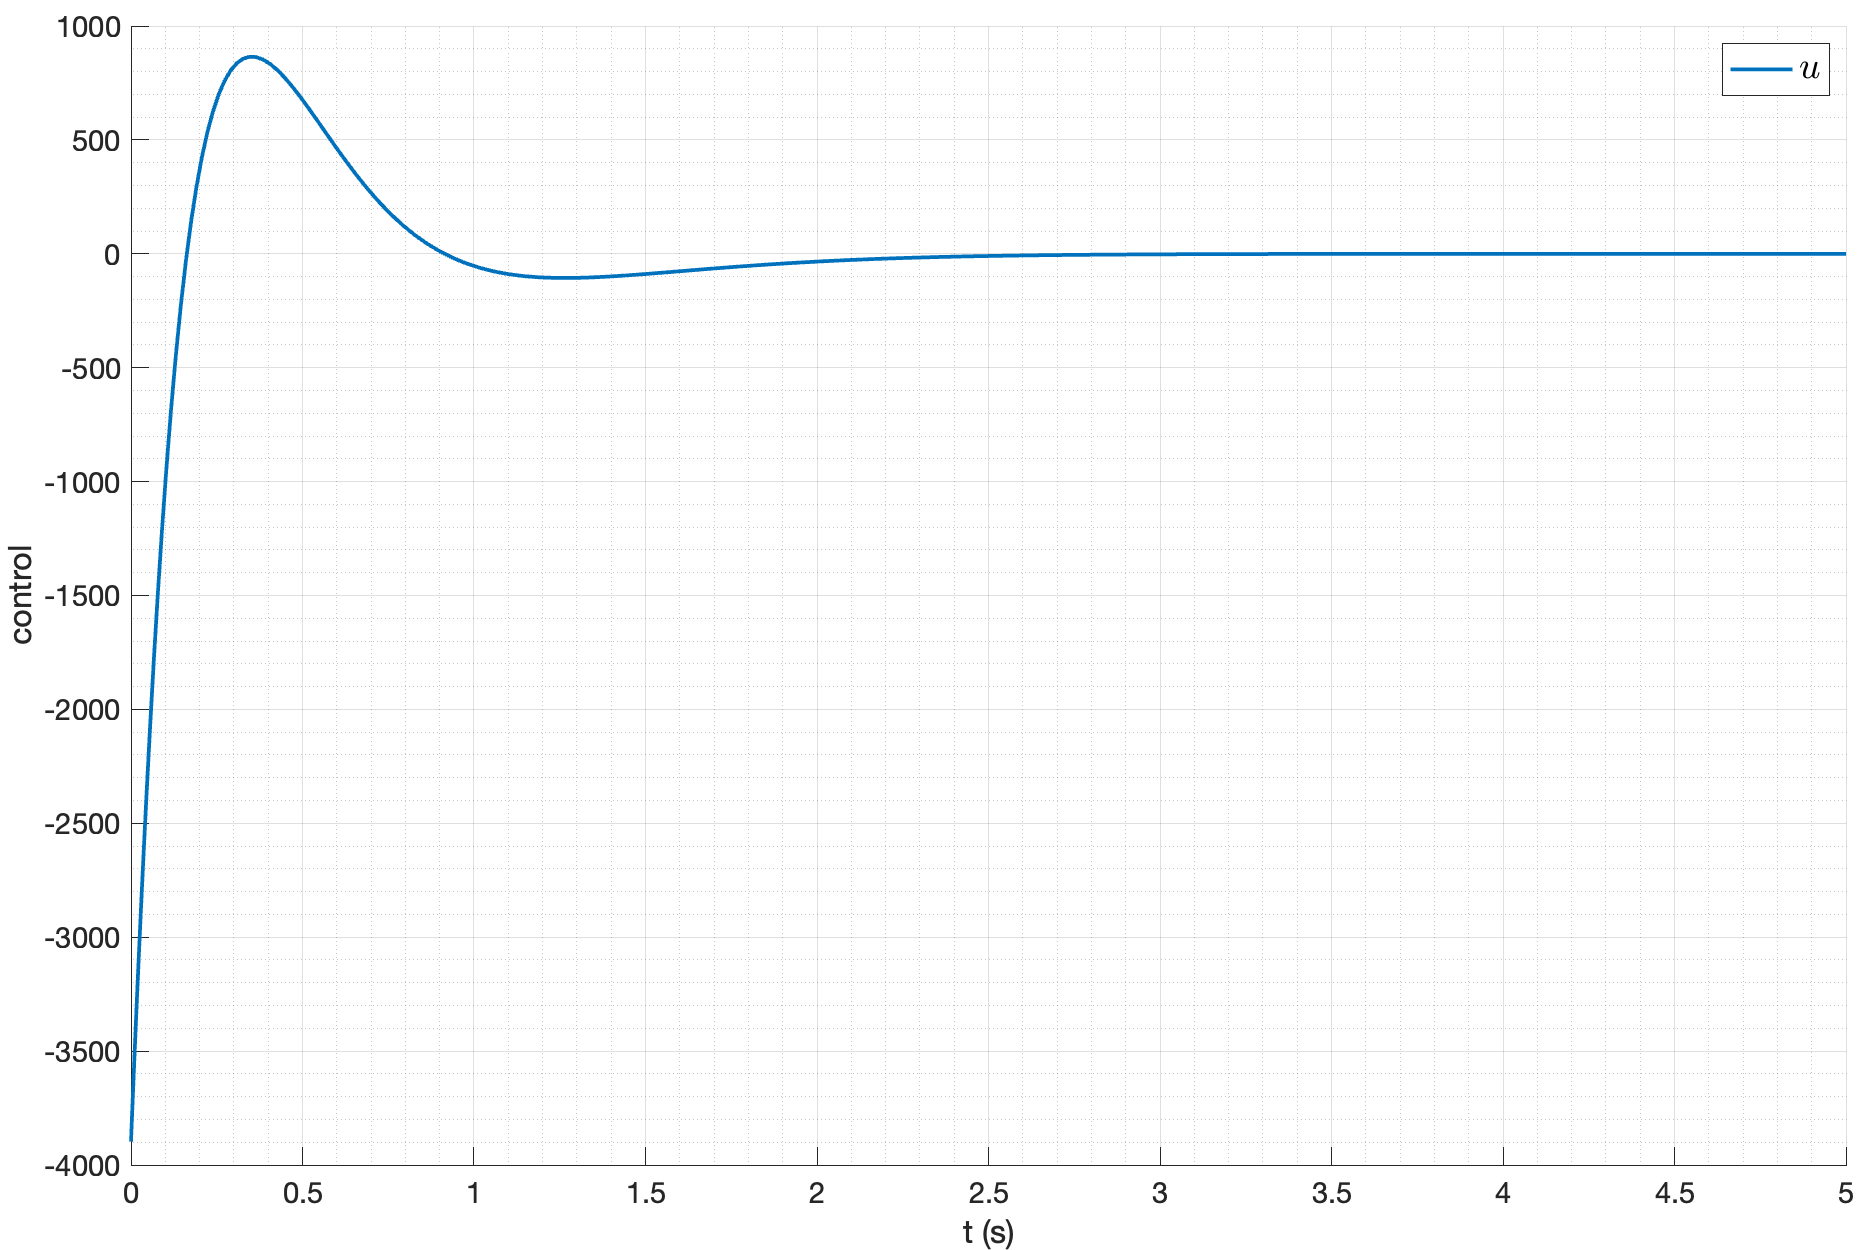
\includegraphics[width=0.8\textwidth]{media/plots/modal_controllers/modal_control_u_1.png}
    \caption{Управляющее воздействие нелинейной модели системы с модальным регулятором при $k = -4$}
    \label{fig:modal_controlers_1_u}
\end{figure}
\begin{figure}[ht!]
    \centering
    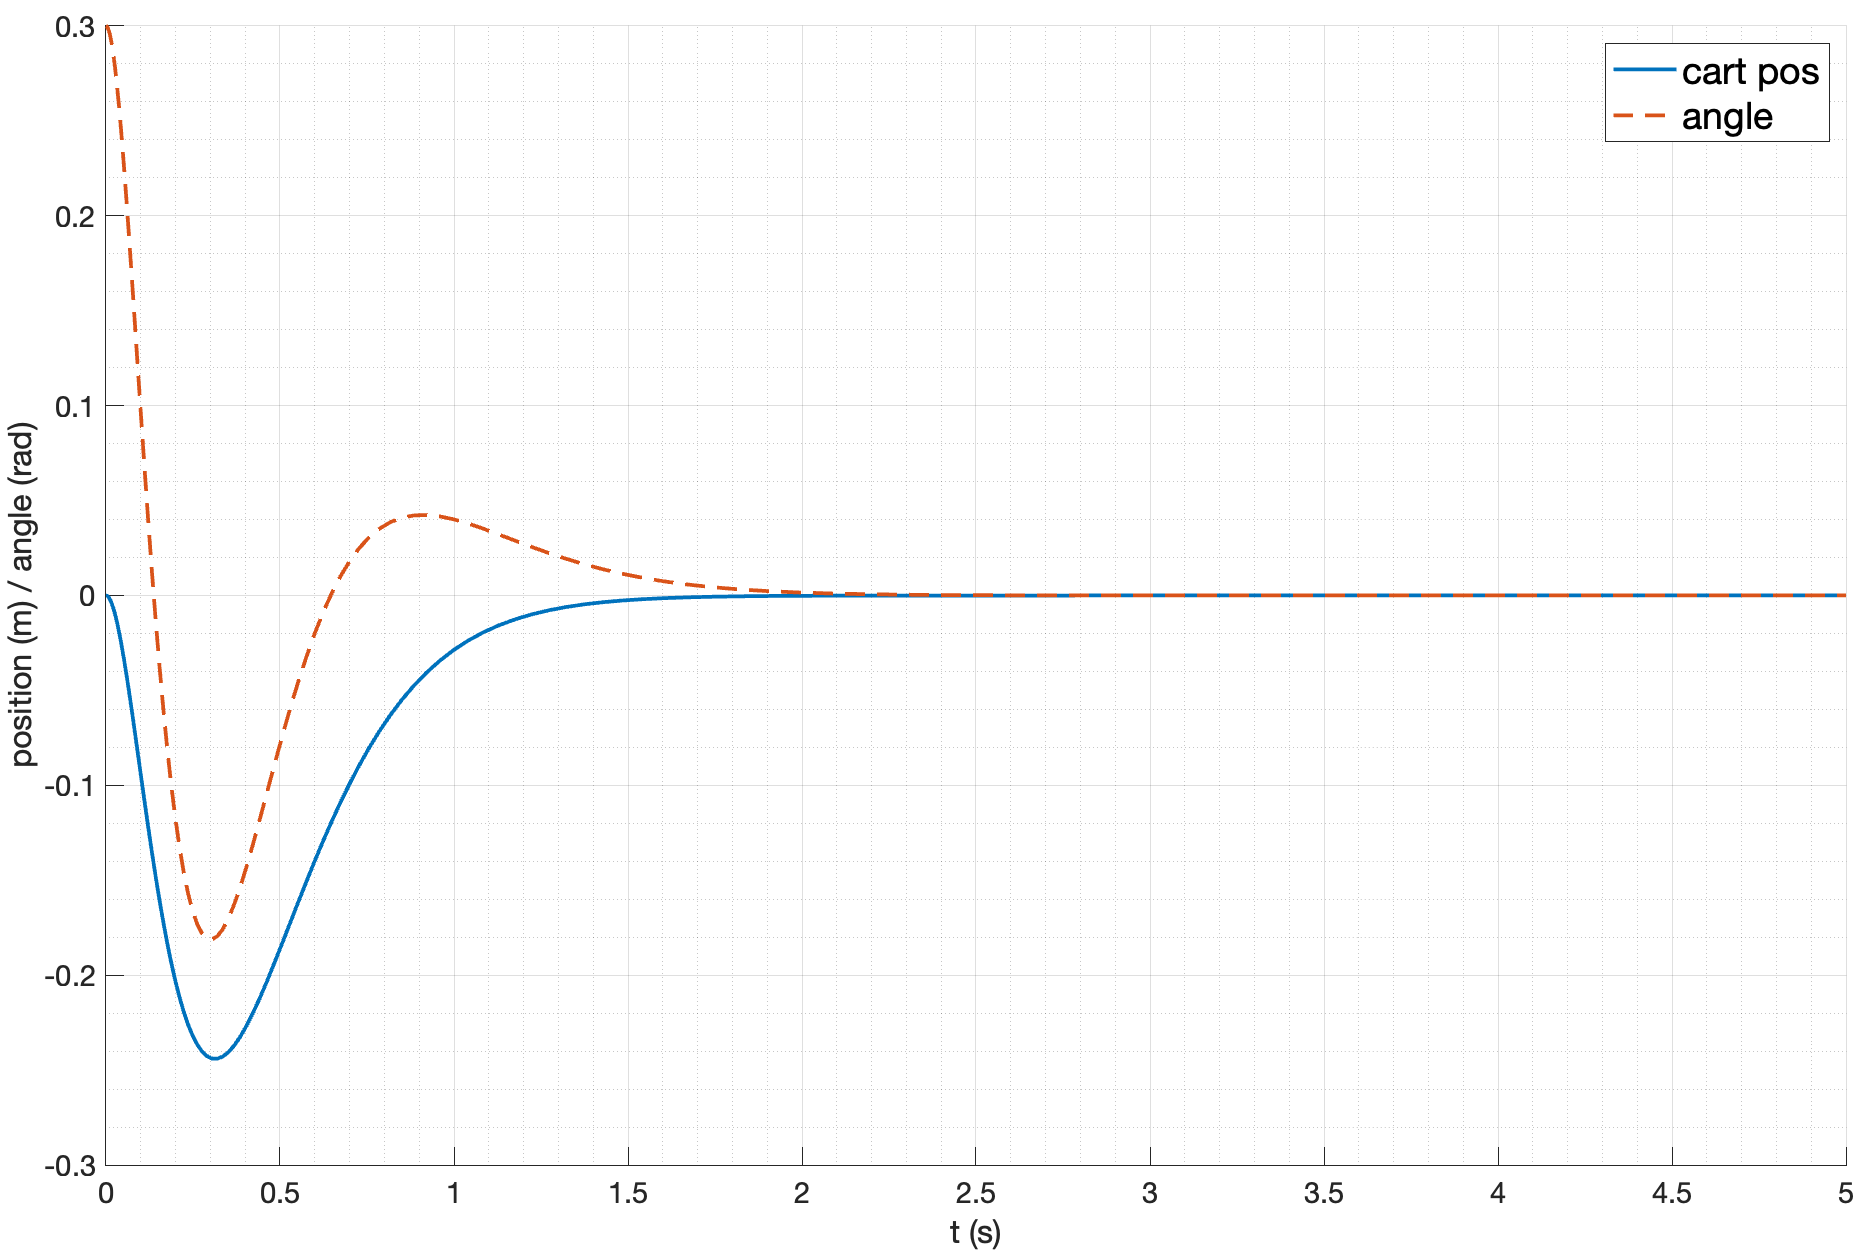
\includegraphics[width=0.8\textwidth]{media/plots/modal_controllers/modal_control_out_2.png}
    \caption{Результаты моделирования нелинейной модели системы с модальным регулятором при $k = -6$}
    \label{fig:modal_controlers_2_out}
\end{figure}
\begin{figure}[ht!]
    \centering
    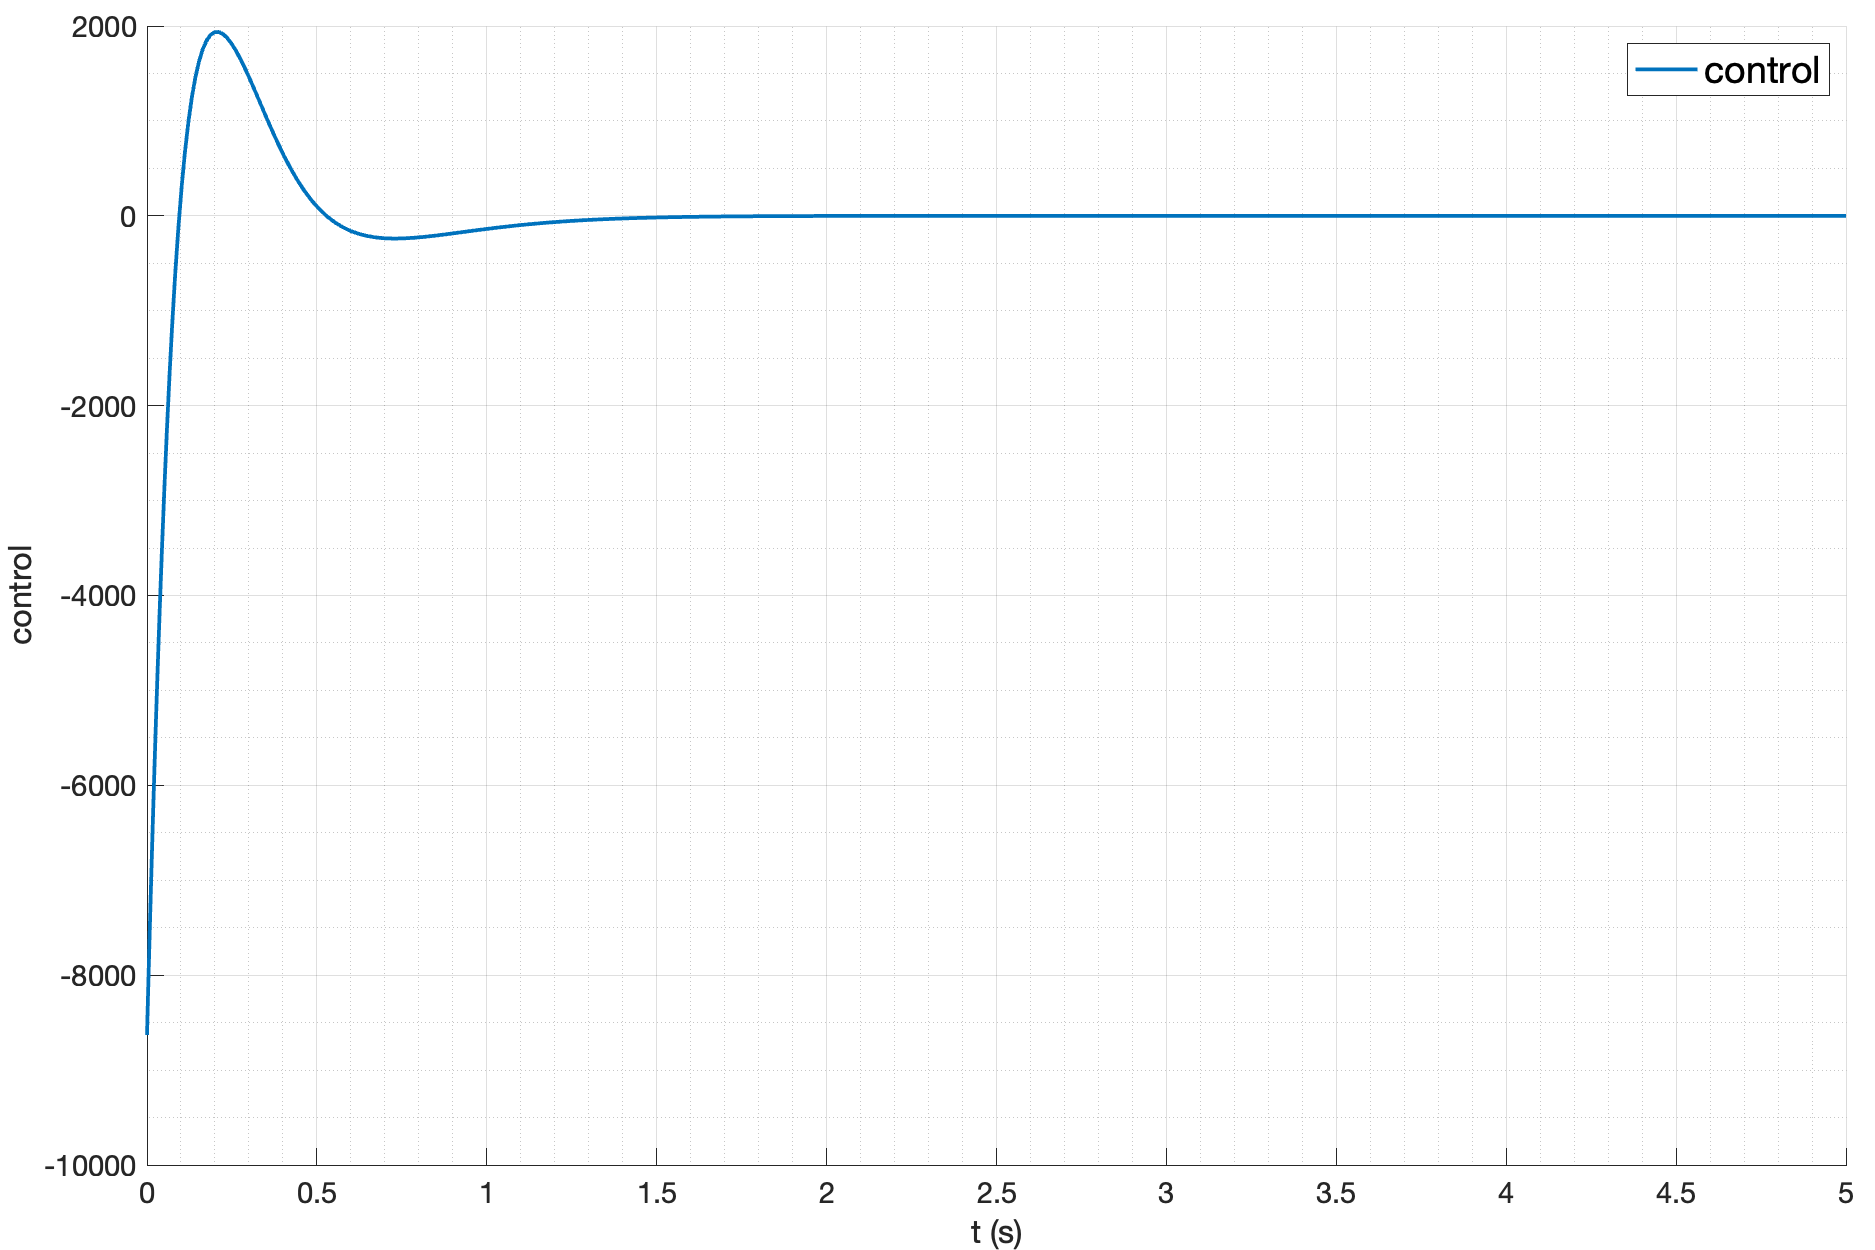
\includegraphics[width=0.8\textwidth]{media/plots/modal_controllers/modal_control_u_2.png}
    \caption{Управляющее воздействие нелинейной модели системы с модальным регулятором при $k = -6$}
    \label{fig:modal_controlers_2_u}
\end{figure}
\begin{figure}[ht!]
    \centering
    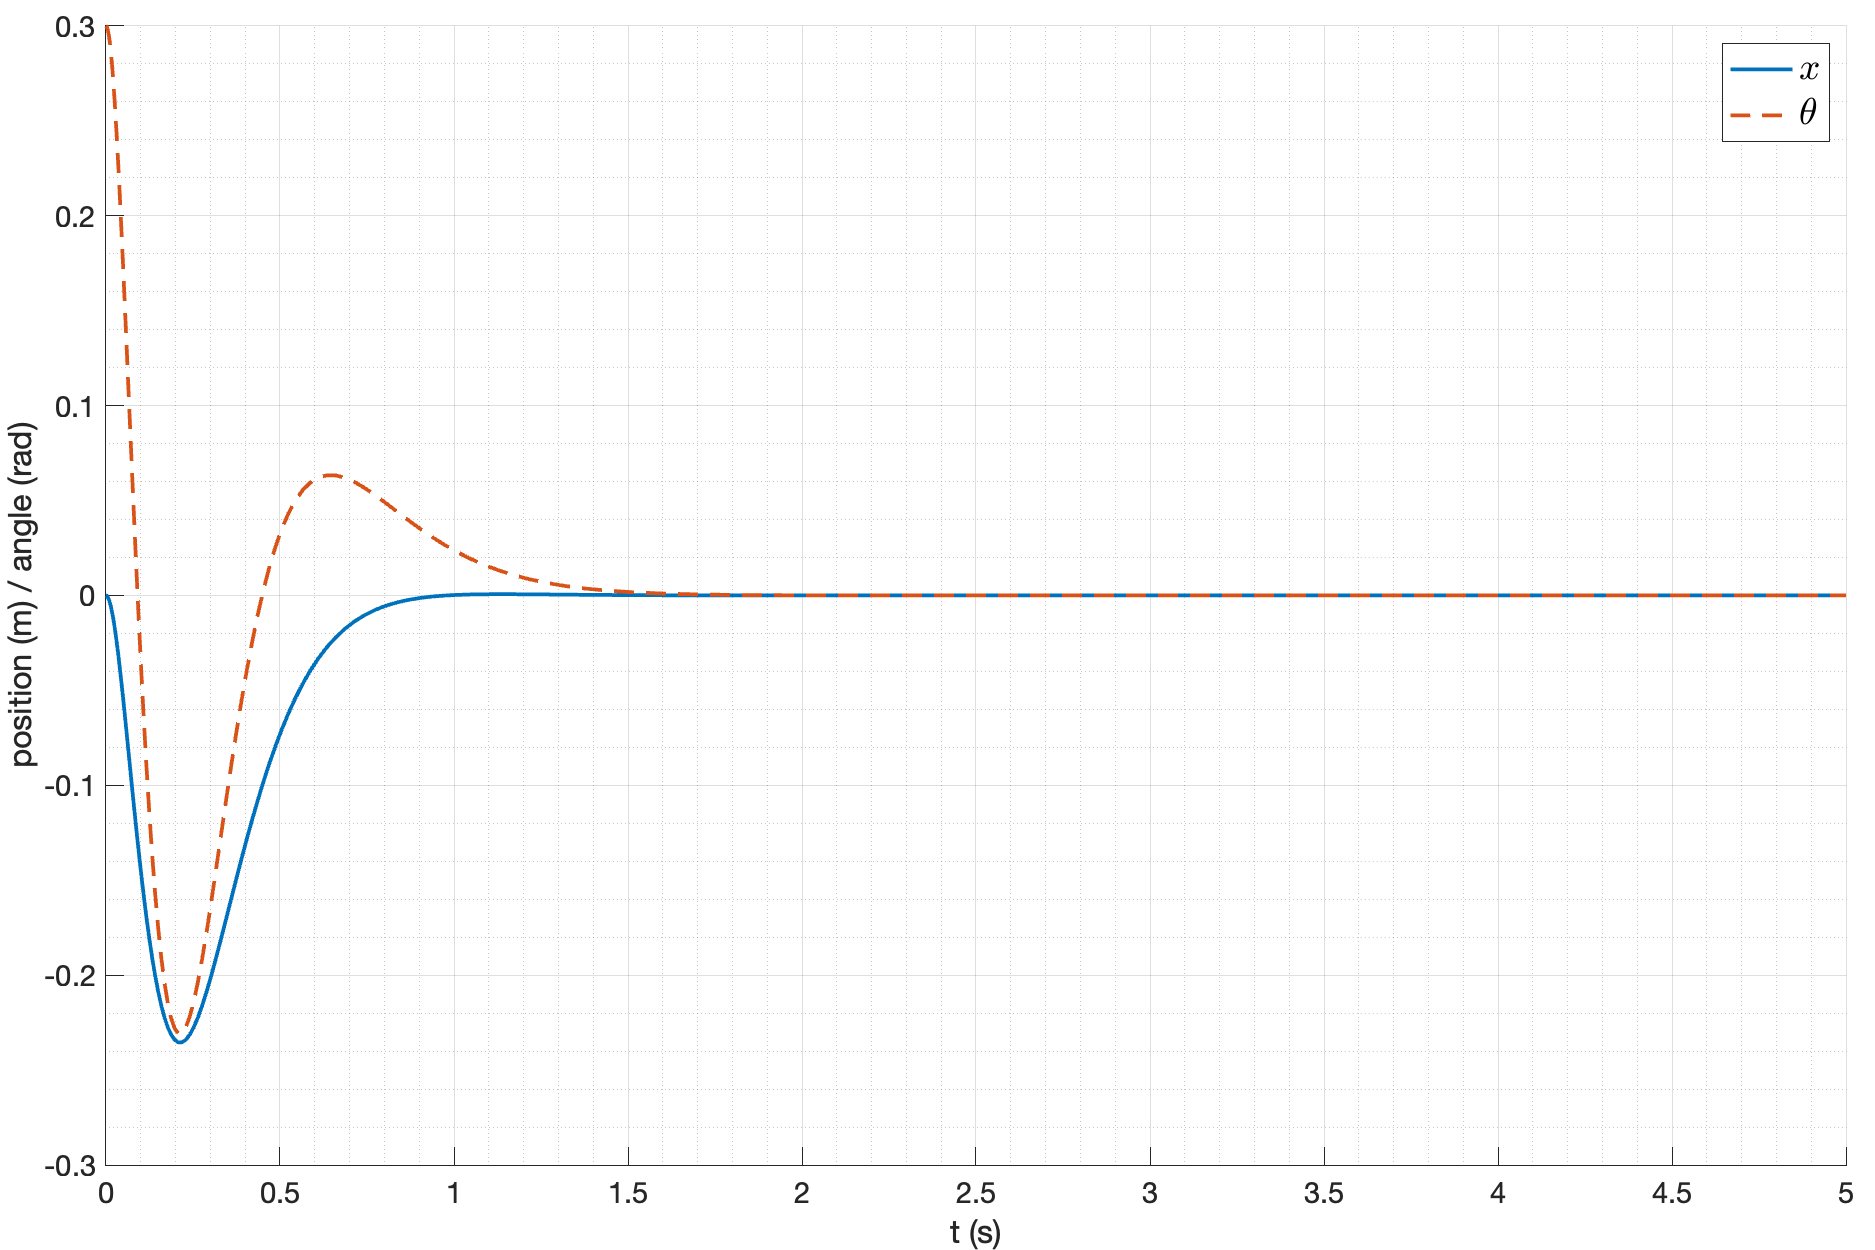
\includegraphics[width=0.8\textwidth]{media/plots/modal_controllers/modal_control_out_3.png}
    \caption{Результаты моделирования нелинейной модели системы с модальным регулятором при $k = -8$}
    \label{fig:modal_controlers_3_out}
\end{figure}
\begin{figure}[ht!]
    \centering
    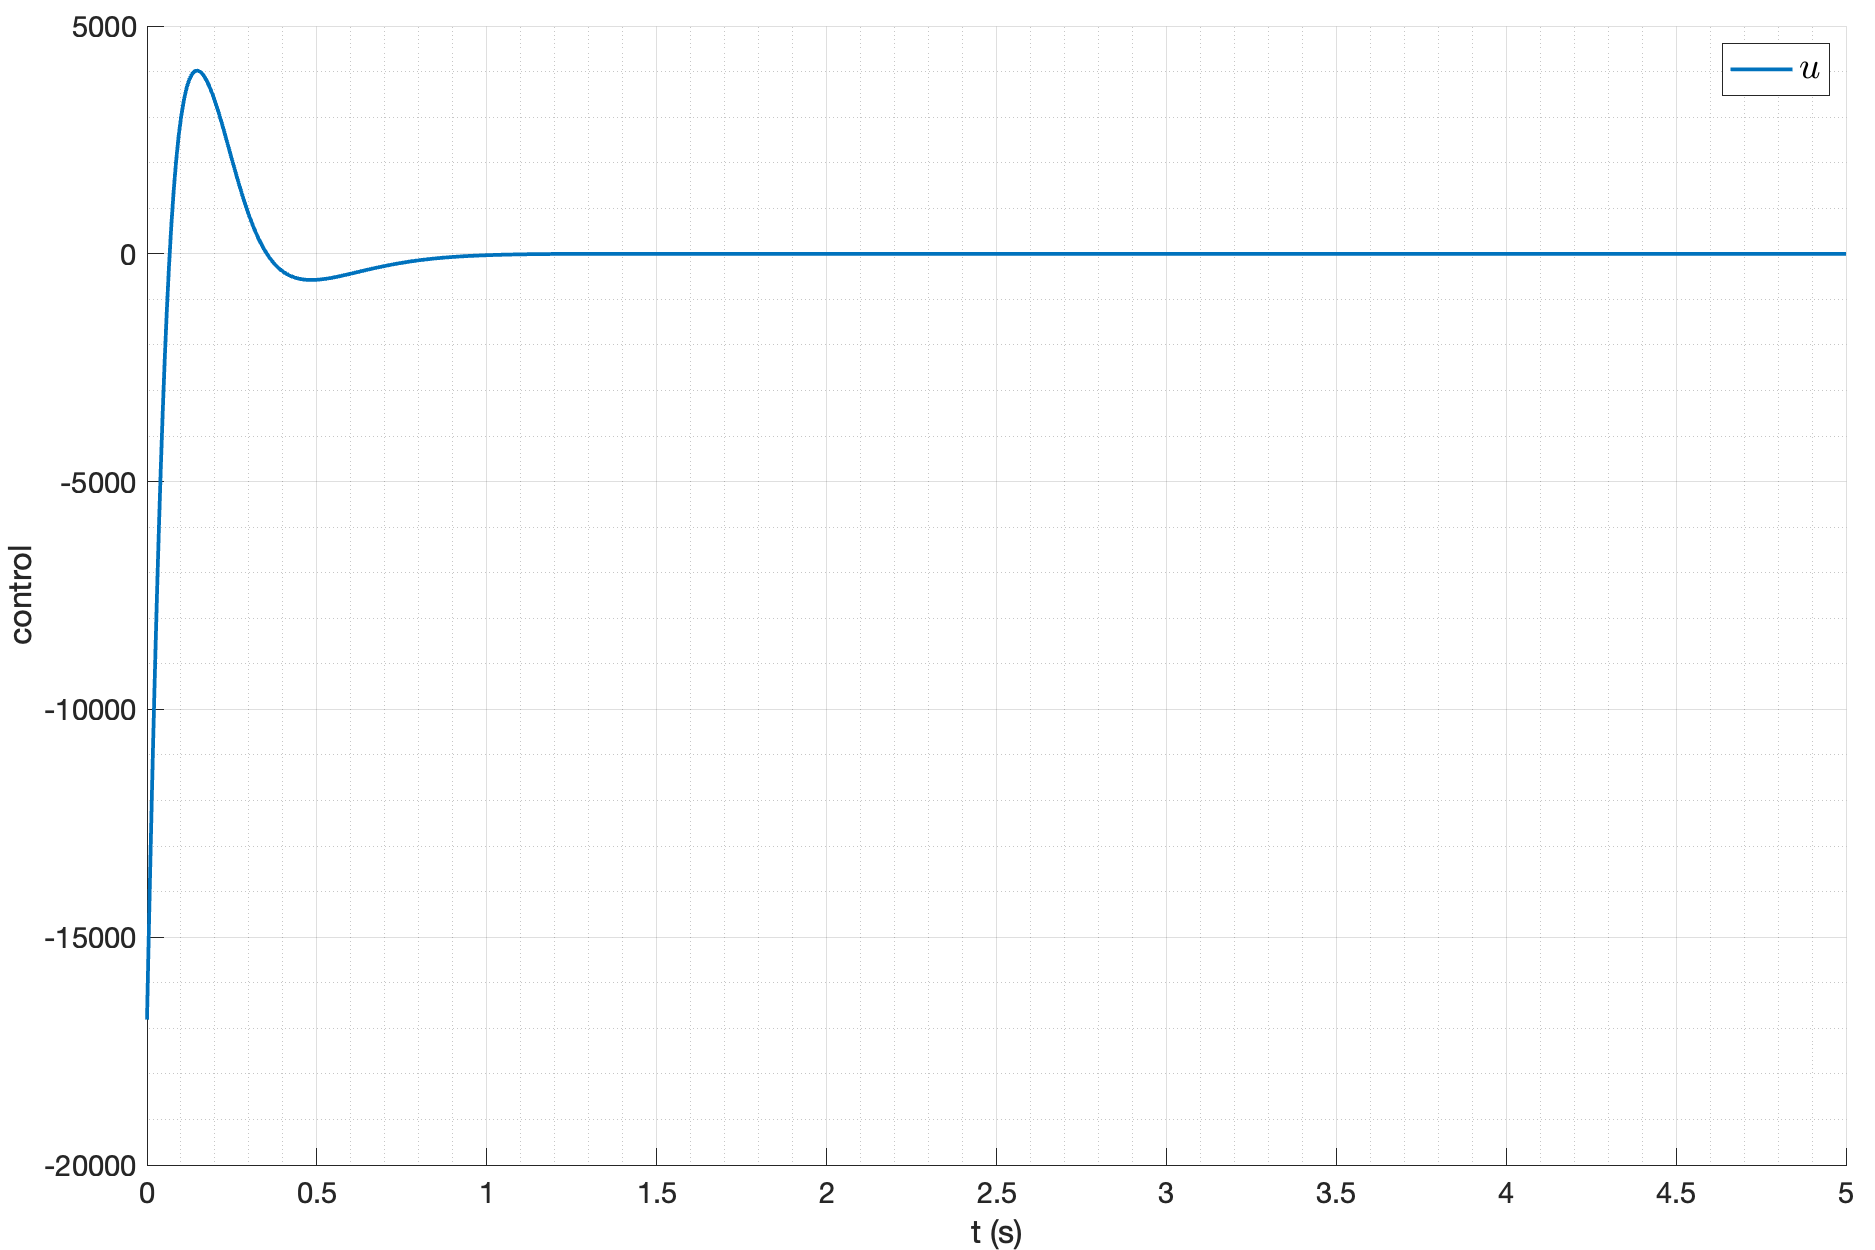
\includegraphics[width=0.8\textwidth]{media/plots/modal_controllers/modal_control_u_3.png}
    \caption{Управляющее воздействие нелинейной модели системы с модальным регулятором при $k = -8$}
    \label{fig:modal_controlers_3_u}
\end{figure}
\begin{figure}[ht!]
    \centering
    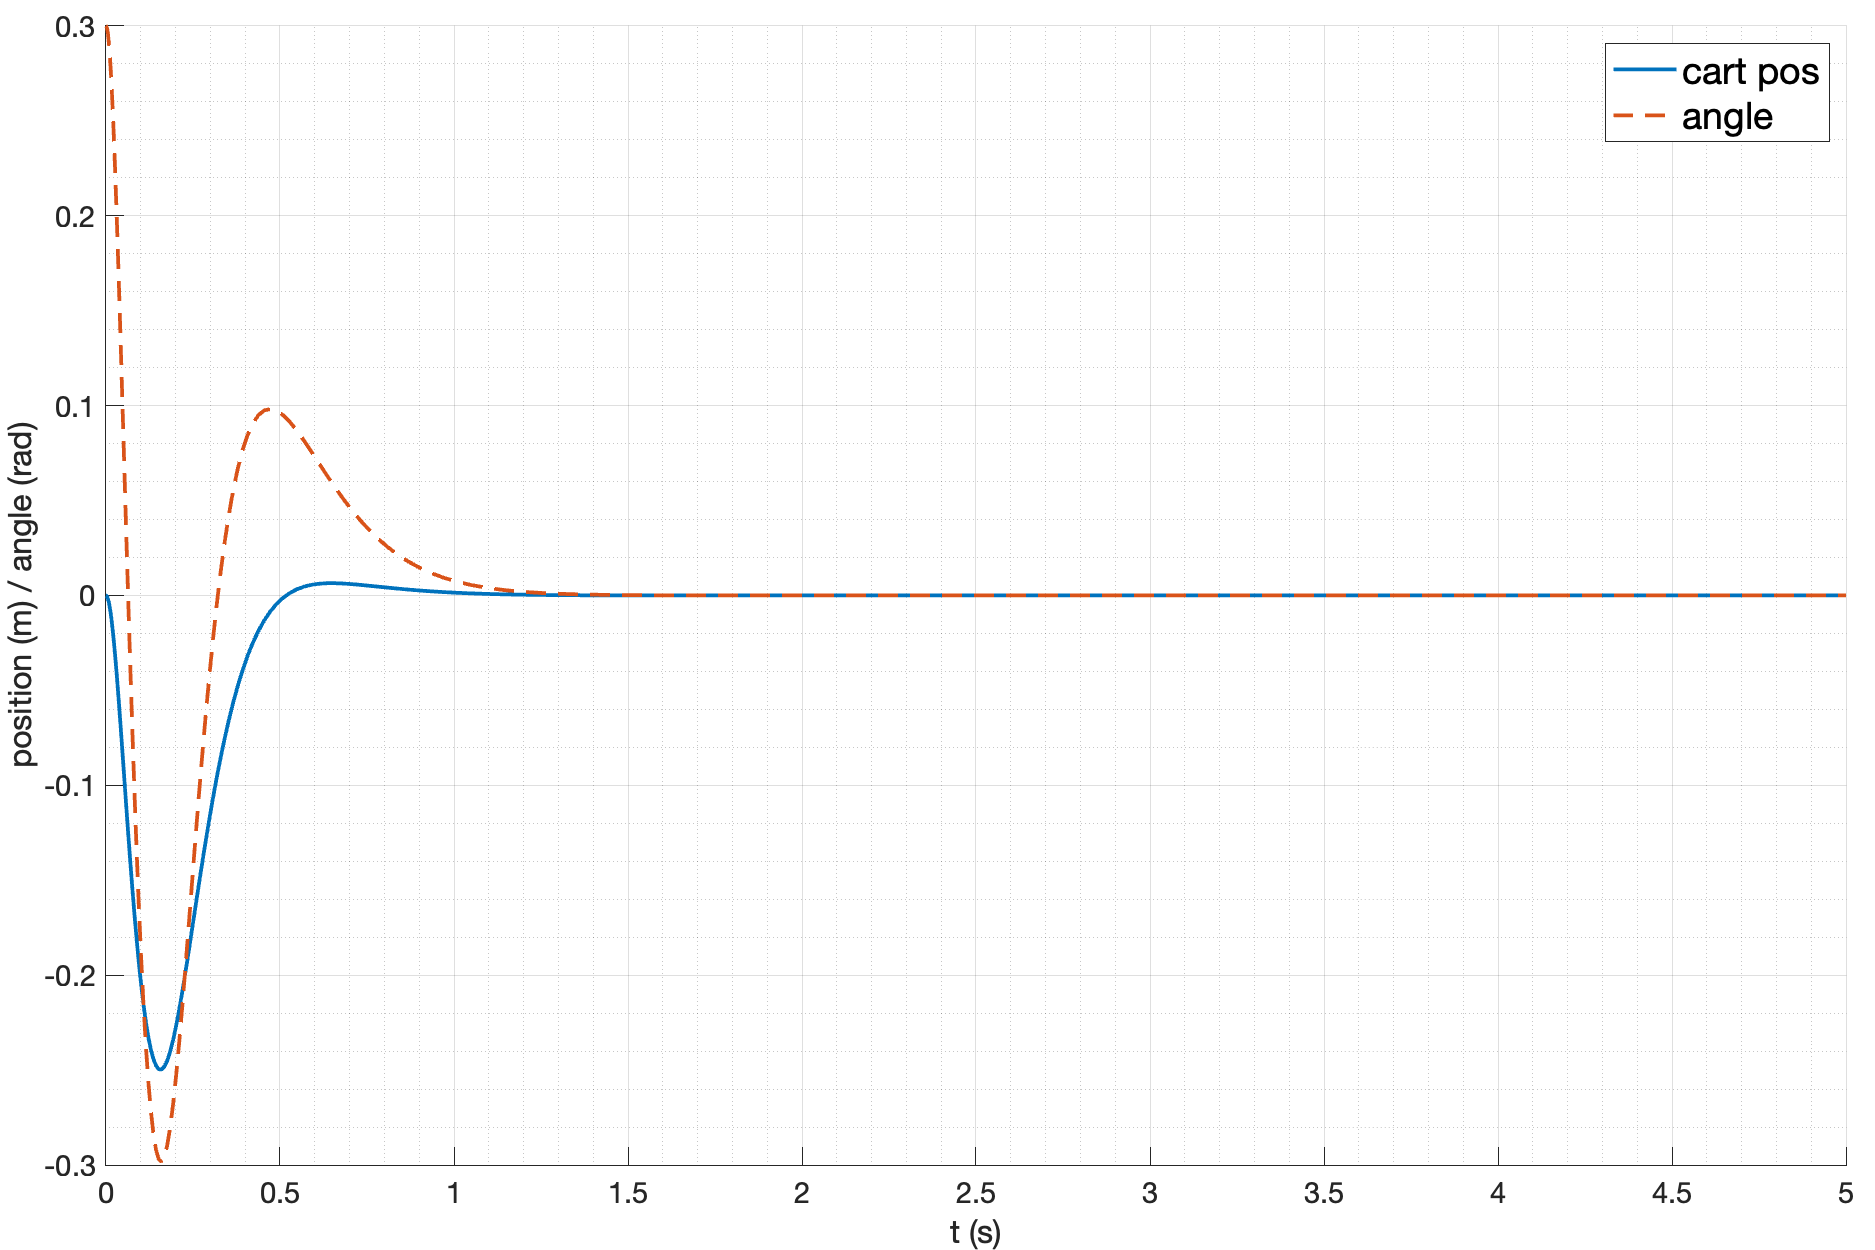
\includegraphics[width=0.8\textwidth]{media/plots/modal_controllers/modal_control_out_4.png}
    \caption{Результаты моделирования нелинейной модели системы с модальным регулятором при $k = -10$}
    \label{fig:modal_controlers_4_out}
\end{figure}
\begin{figure}[ht!]
    \centering
    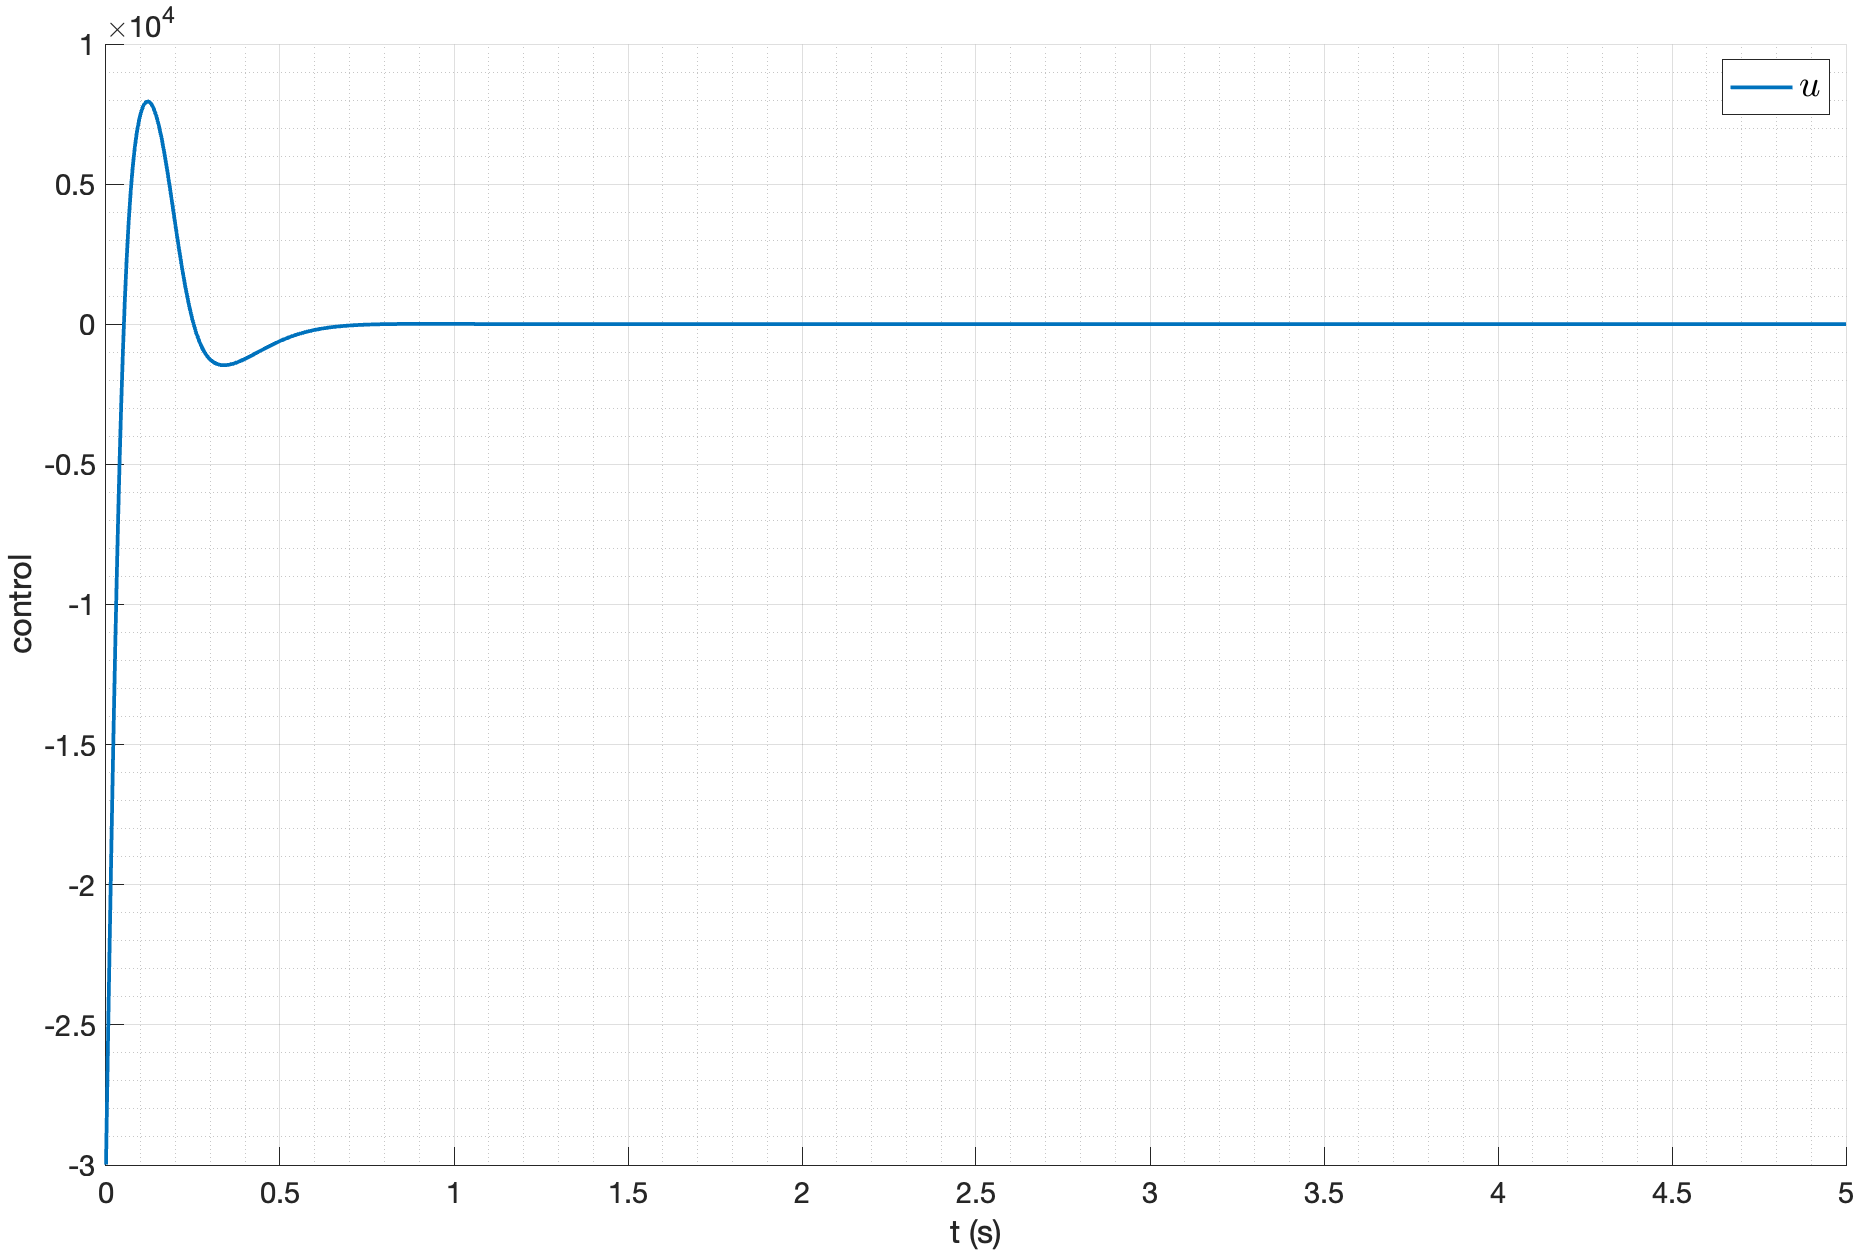
\includegraphics[width=0.8\textwidth]{media/plots/modal_controllers/modal_control_u_4.png}
    \caption{Управляющее воздействие нелинейной модели системы с модальным регулятором при $k = -10$}
    \label{fig:modal_controlers_4_u}
\end{figure}
Можно заметить, что при увеличении модуля собственных чисел замкнутой системы, время переходного процесса
сокращается, а перегулирование отклонения маятника увеличивается, максимальный модуль управляющего воздействия 
тоже увеличивается с увеличением модуля собственных чисел. Численные результаты сравнения приведены в таблице \ref{tab:modal_control_cmp}. 

\begin{table}[ht!]
    \centering
    \begin{tabular}{|c|c|c|c|c|}
        \hline
        $k$ & $t_{\text{set}}$, с & $M_{\theta}$ & $M_{x}$ & $\max{|u|}$ \\
        \hline
        -4 & 3.1 & 0.15 & 0.32 & 3800 \\
        \hline
        -6 & 2.2 & 0.18 & 0.24 & 9100 \\
        \hline
        -8 & 1.6 & 0.23 & 0.24 & 17000 \\
        \hline
        -10 & 1.4 & 0.3 & 0.25 & 30000 \\
        \hline
    \end{tabular}
    \caption{Сравнение регуляторов с различными собственными числами замкнутой системы}
    \label{tab:modal_control_cmp}
\end{table}

Можно заметить, что перегулирование координаты тележки остается практически одинаковым, 
что связано с тем, что угол маятника зависит от скорости и ускорения тележки, а не от ее положения. 

\FloatBarrier
Дополнительно посмотрим на случай замкнутой системы, имеющий спектр $\begin{bmatrix}-0.5 & -0.5 & -4 &- 4\end{bmatrix}$
и сравним ее с системой, имеющей спектр $\begin{bmatrix}-4 & -4 & -4 &- 4\end{bmatrix}$, рассмотренной на рисунке \ref{fig:modal_controlers_1_out}.
Графики результатов моделирования приведены на рисунке \ref{fig:modal_controlers_5_out} -- \ref{fig:modal_controlers_5_u}. 
\begin{figure}[ht!]
    \centering
    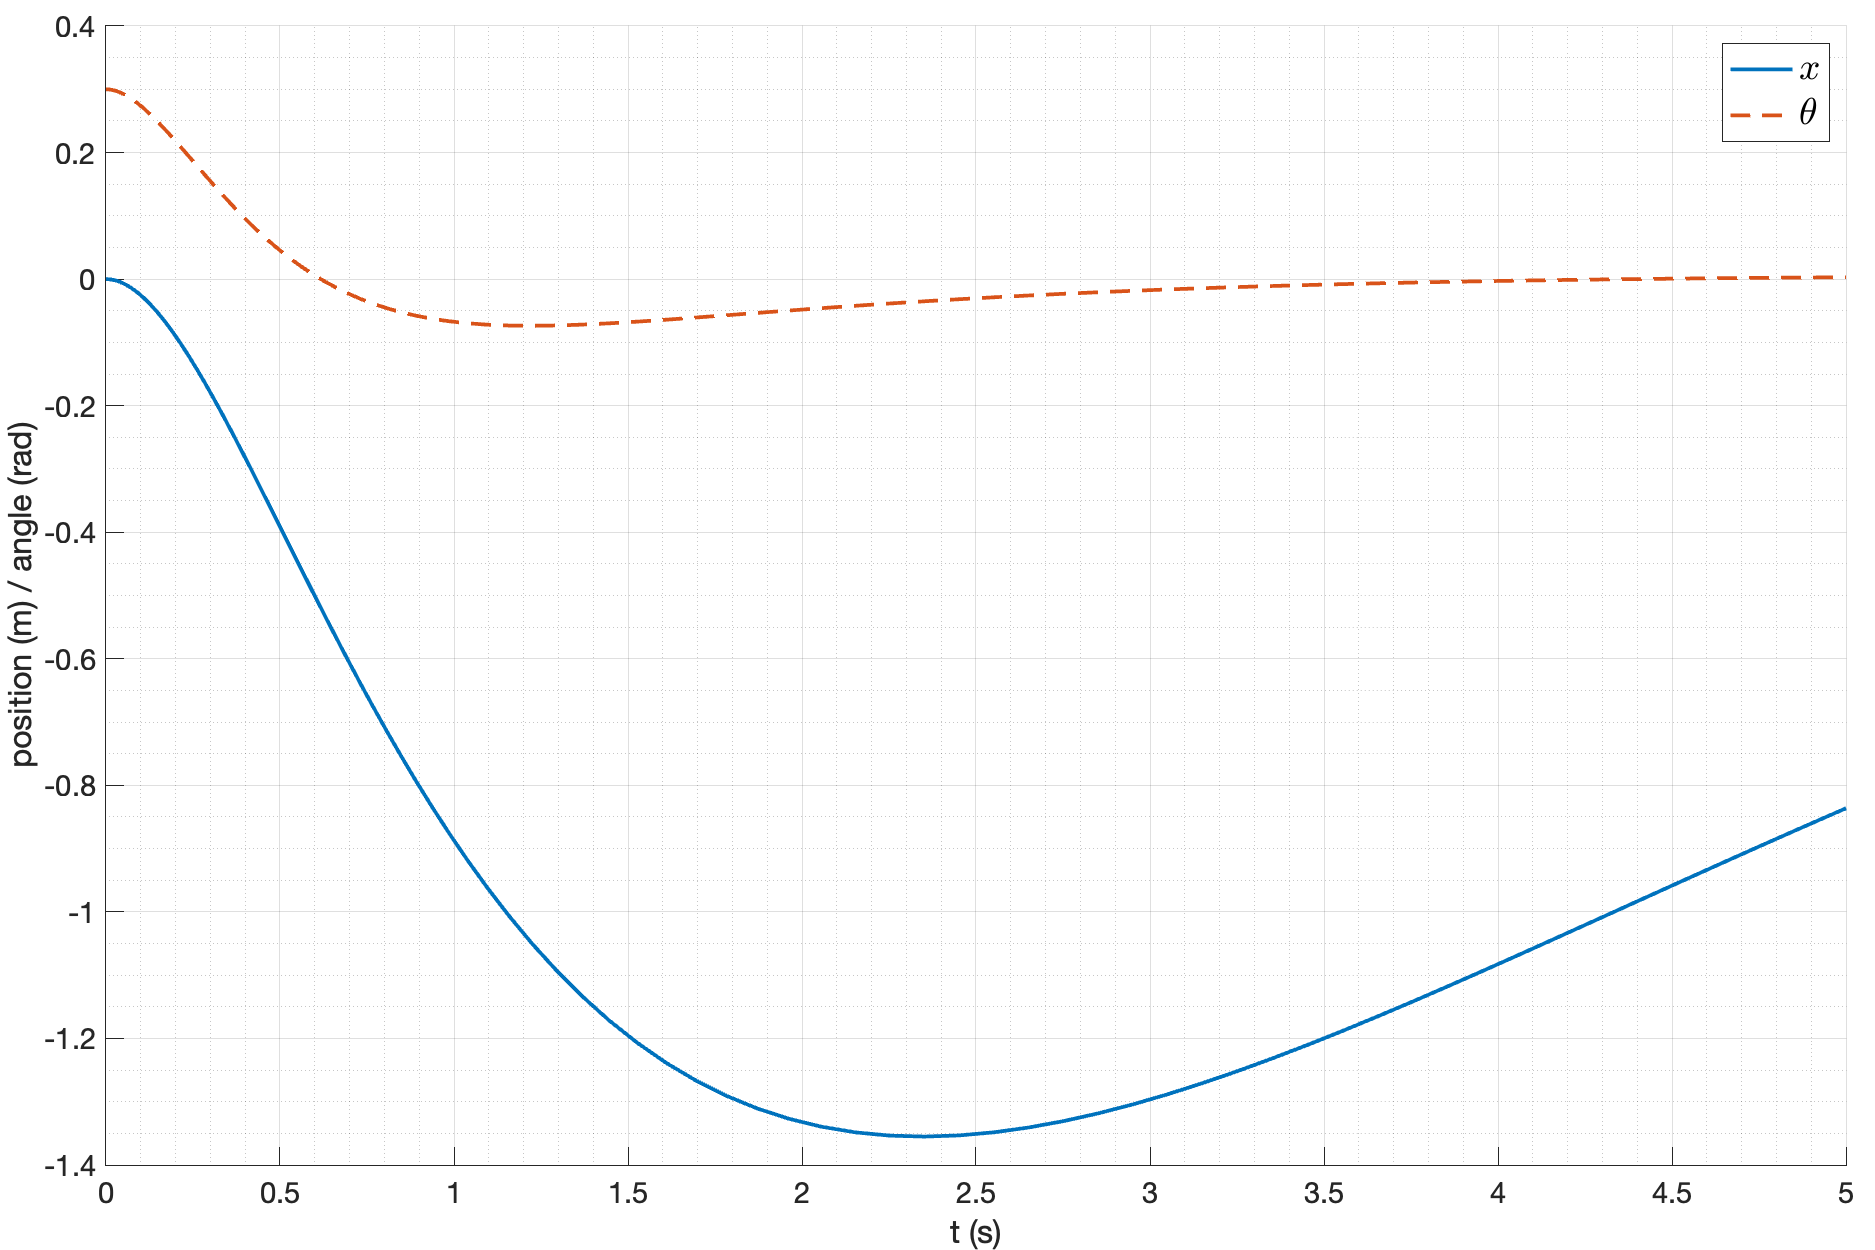
\includegraphics[width=0.8\textwidth]{media/plots/modal_controllers/modal_control_out_5.png}
    \caption{Результаты моделирования нелинейной модели системы со спектром $\begin{bmatrix}-0.5 & -0.5 & -4 &- 4\end{bmatrix}$}
    \label{fig:modal_controlers_5_out}
\end{figure}
\begin{figure}[ht!]
    \centering
    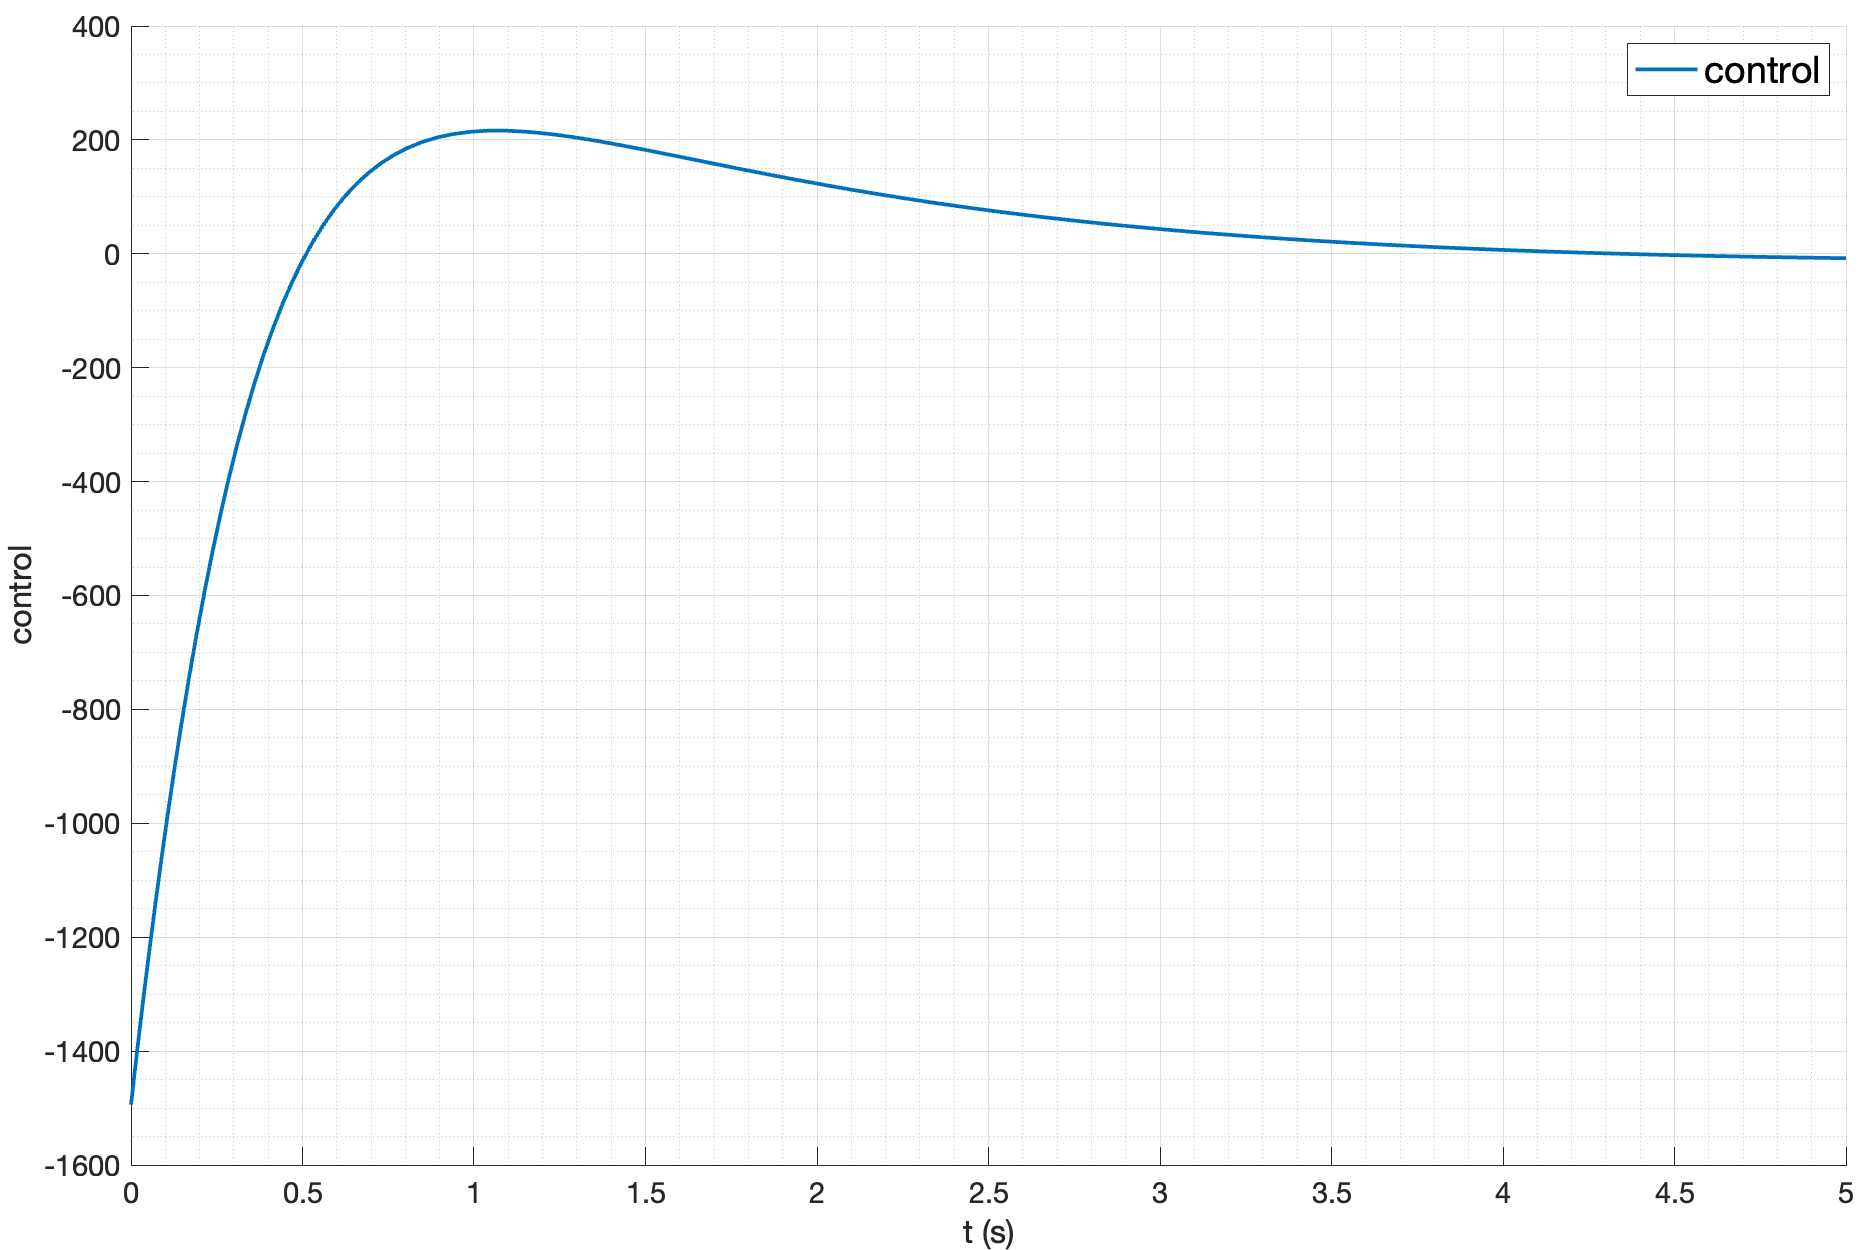
\includegraphics[width=0.8\textwidth]{media/plots/modal_controllers/modal_control_u_5.png}
    \caption{Управляющее воздействие нелинейной модели системы со спектром $\begin{bmatrix}-0.5 & -0.5 & -4 &- 4\end{bmatrix}$}
    \label{fig:modal_controlers_5_u}
\end{figure}
Видно, что при уменьшении первых двух собственных чисел замкнутой системы, время переходного процесса для 
координаты тележки сильно увеличивается, а для угла отклонения маятника практически не меняется, при этом 
управление тоже становится меньше. При уменьшении первых двух собственных чисел произошло влияние на первые 
два собственные вектора системы (\ref{eq:eigenvectors}), которые, в свою очередь, влияют на 
линейное положение тележки, но не на угол отклонения маятника. Таким образом, можно сделать вывод, что 
с использованием модального управления можно влиять на динамику системы \textit{по отдельности}, изменяя 
собственные числа для каждого из собственных векторов.

\subsection{Наблюдатель полного порядка}
Рассмотрим наблюдатель полного порядка,, основанный на линейной модели системы: 
\begin{equation}
    \begin{cases}
        \dot{\hat{x}} = A\hat{x} + Bu + L(y - C\hat{x})\\
        \hat{y} = C\hat{x}
    \end{cases}
\end{equation}
где $L$ -- матрица коррекции наблюдателя. 

Для синтеза наблюдателя воспользуемся уравнением Сильвестра, решение которого будем находить с помощью
пакета \texttt{cvx} в MATLAB.
\begin{equation}
    \begin{cases}
        \Gamma Q - QA = YC \\ 
        L = QY^{-1}
    \end{cases}
\end{equation}
где $\Gamma$ -- матрица с желаемыми собственными числами. 

Синтезируем наблюдатель с желаемым спектром $\{-3, -3, -3, -3\}$. 
Решим уравнение Сильвестра с помощью пакета \texttt{cvx} в MATLAB, в результате получаем матрицу наблюдателя $L$:
\begin{equation}
    L = \begin{bmatrix}
    3.91  & 3.91 \\ 
    2.07  & 2.07 \\ 
    -15.91  & -15.91 \\ 
    -82.41  & -82.41 \\ 
    \end{bmatrix}
\end{equation}
Проверим правильность полученного результата, вычислив собственные числа замкнутой системы $A + LC$: 
\begin{equation}
    \sigma(A + LC) = \begin{bmatrix}
    -3.00 \\ 
    -3.00 \\ 
    -3.00 \\ 
    -3.00 \\ 
    \end{bmatrix}
\end{equation}
Проверим полученный наблюдатель, сравнив его выход с реальным состоянием нелинейной системы. В качестве регулятора 
выберем регулятор со спектром $\begin{bmatrix}-6 & -6 & -6 & -6\end{bmatrix}$, рассмотренный ранее. В качестве 
начальных условий возьмем $\theta_0 = 0.3$ для системы и $\hat{X}_0 = 0$ для наблюдателя.

Схема наблюдателя приведена на рисунке \ref{fig:observer_scheme}. Схема включения наблюдателя в систему 
показана на рисунке \ref{fig:observer_system} и рисунках \ref{fig:observer_x_cmp_1_sep}. 
\begin{figure}[ht!]
    \centering
    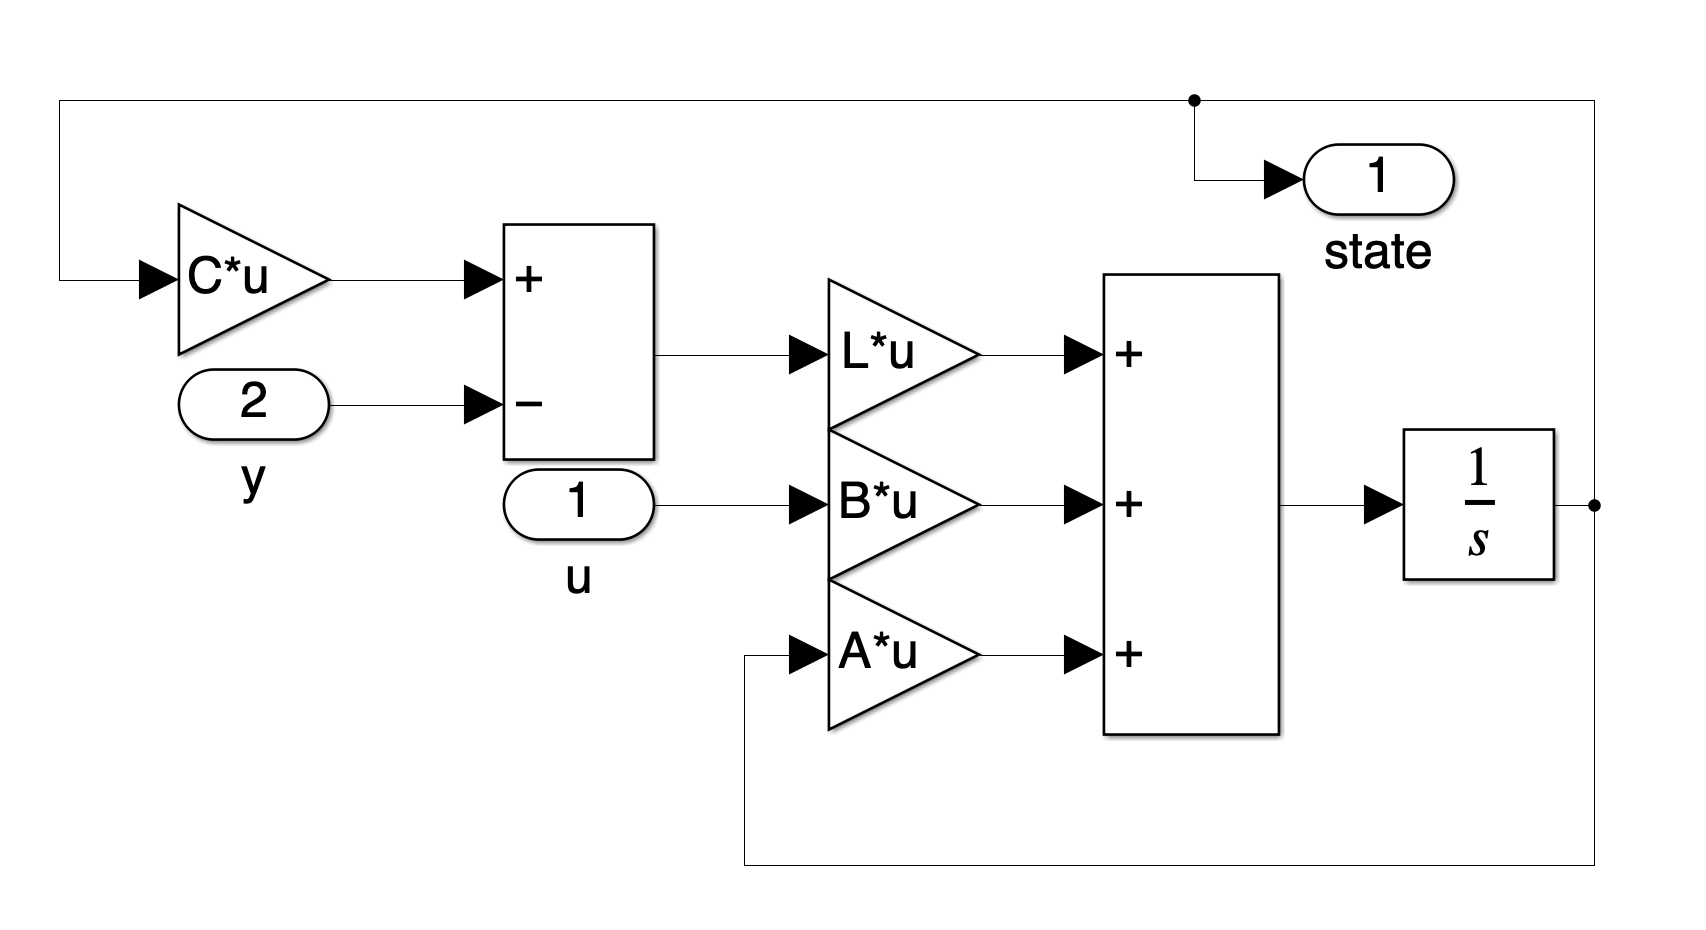
\includegraphics[width=0.7\textwidth]{media/observer_scheme.png}
    \caption{Схема наблюдателя}
    \label{fig:observer_scheme}
\end{figure}
\begin{figure}[ht!]
    \centering
    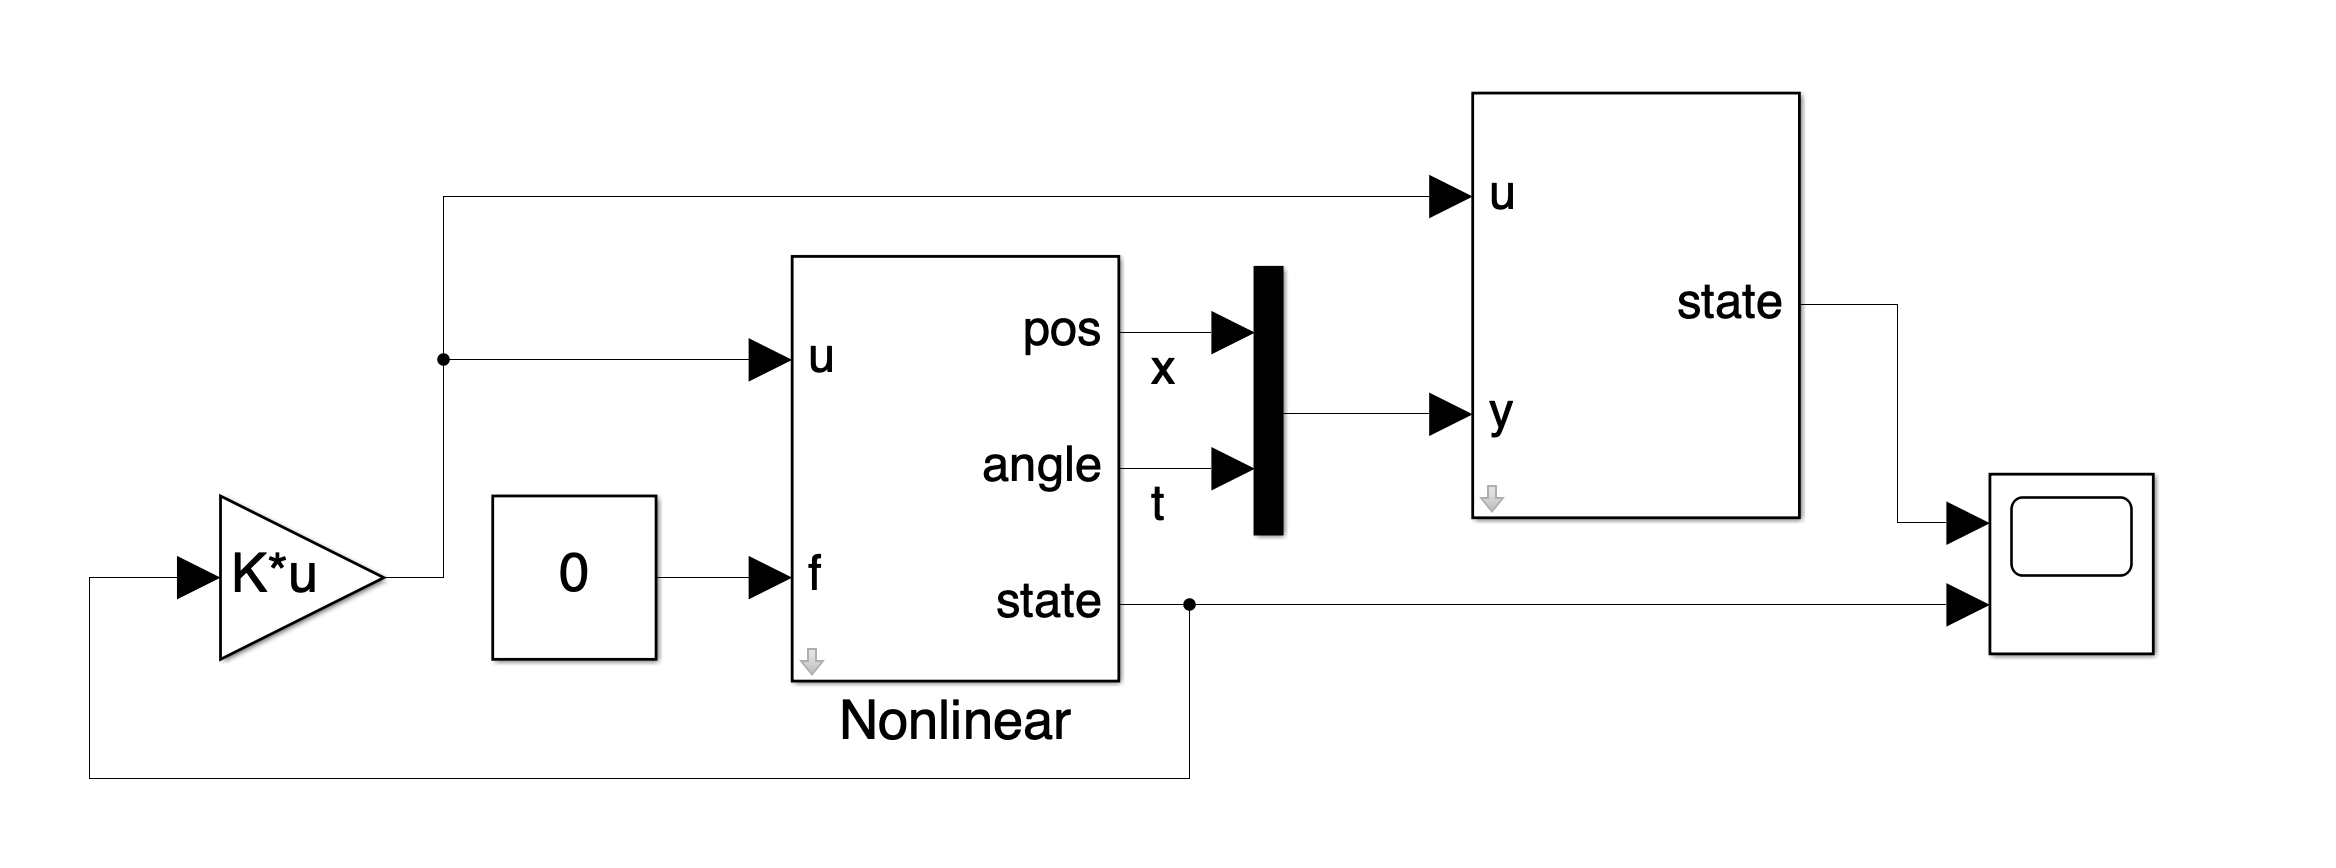
\includegraphics[width=0.7\textwidth]{media/observer_system.png}
    \caption{Схема включения наблюдателя в систему}
    \label{fig:observer_system}
\end{figure}

Результаты моделирования приведены на рисунке \ref{fig:observer_x_1}.
\begin{figure}[ht!]
    \centering
    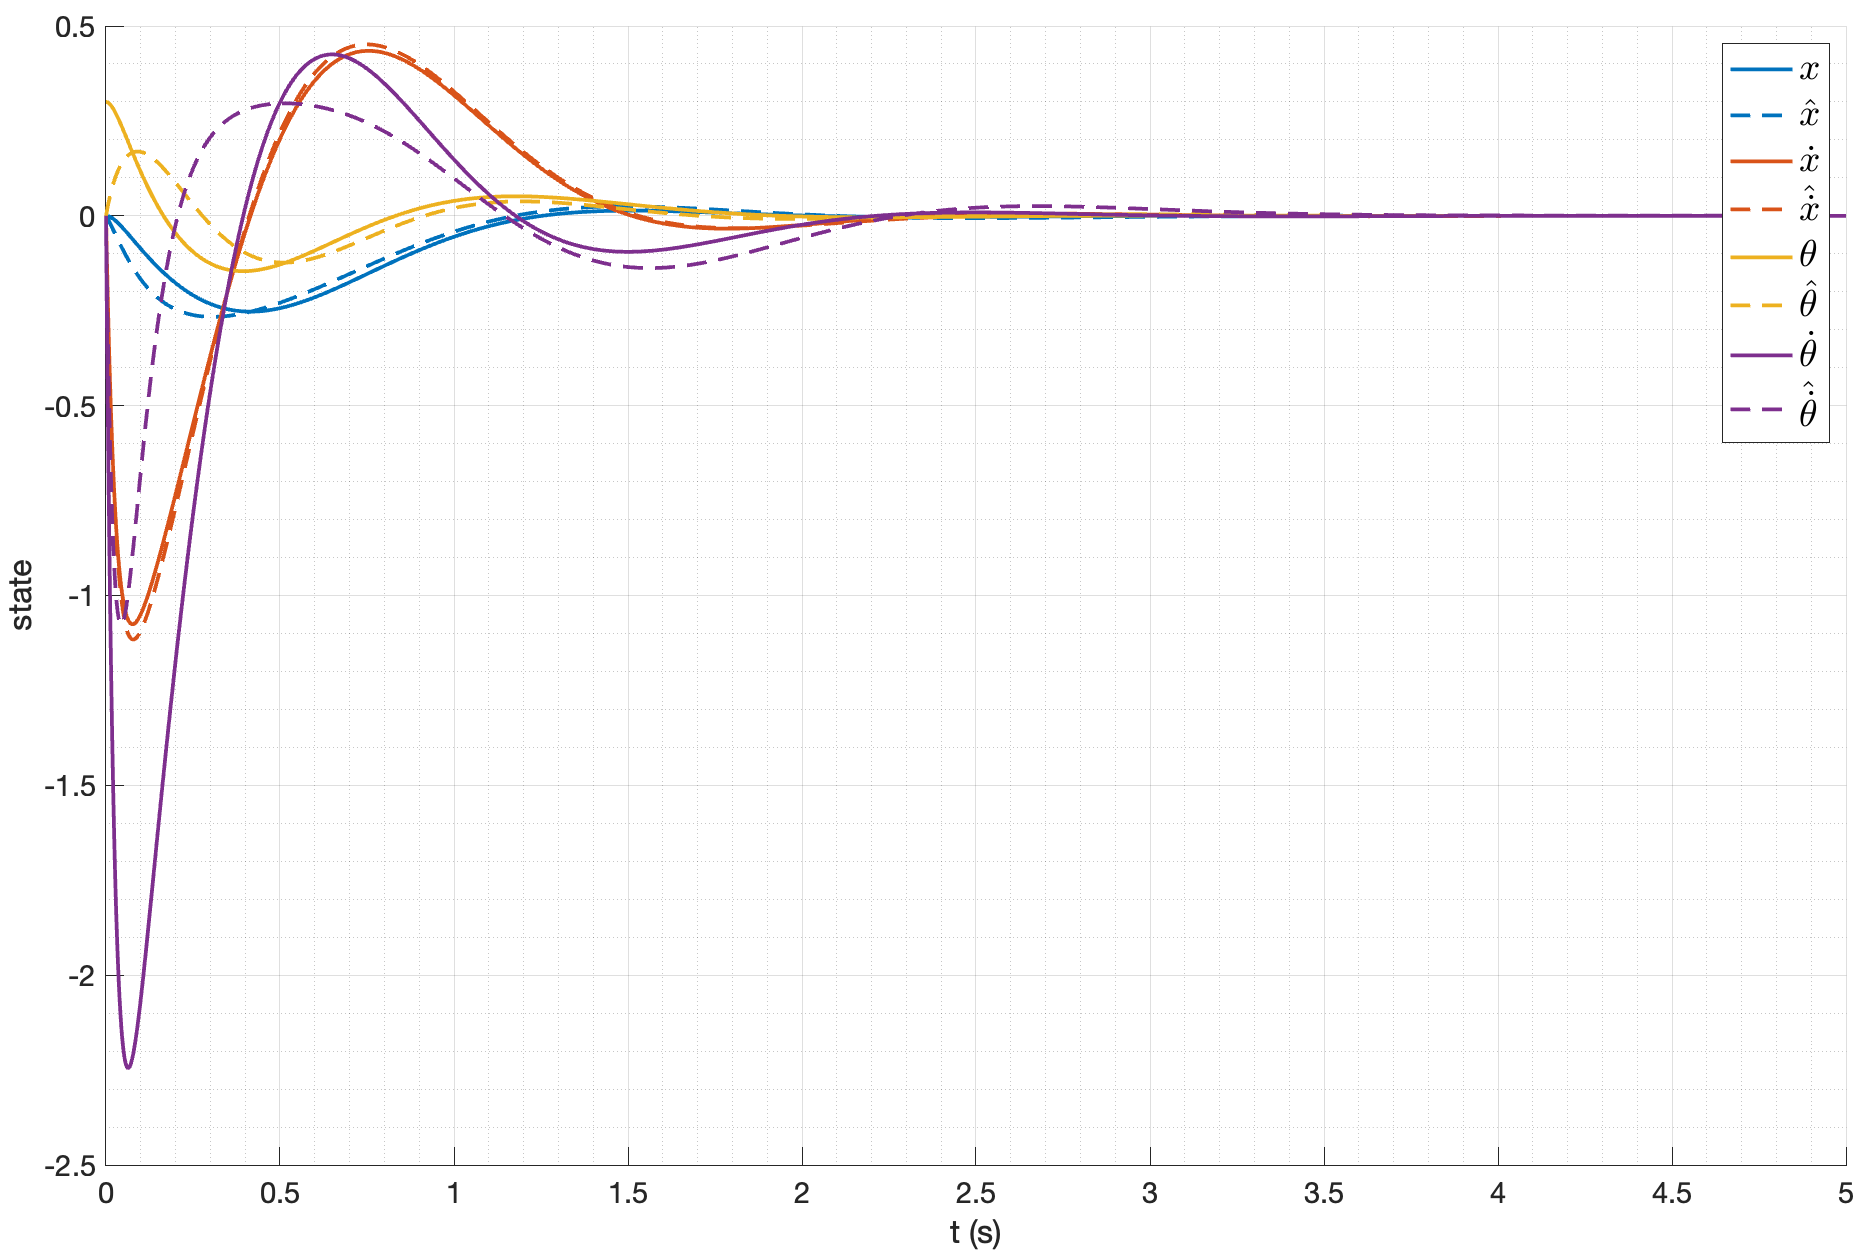
\includegraphics[width=\textwidth]{media/plots/modal_observer/observer_cmp_1.png}
    \caption{Результаты моделирования наблюдателя полного порядка}
    \label{fig:observer_x_1}
\end{figure}
\begin{figure}[ht!]
    \centering
    \begin{subfigure}[b]{0.45\textwidth}
        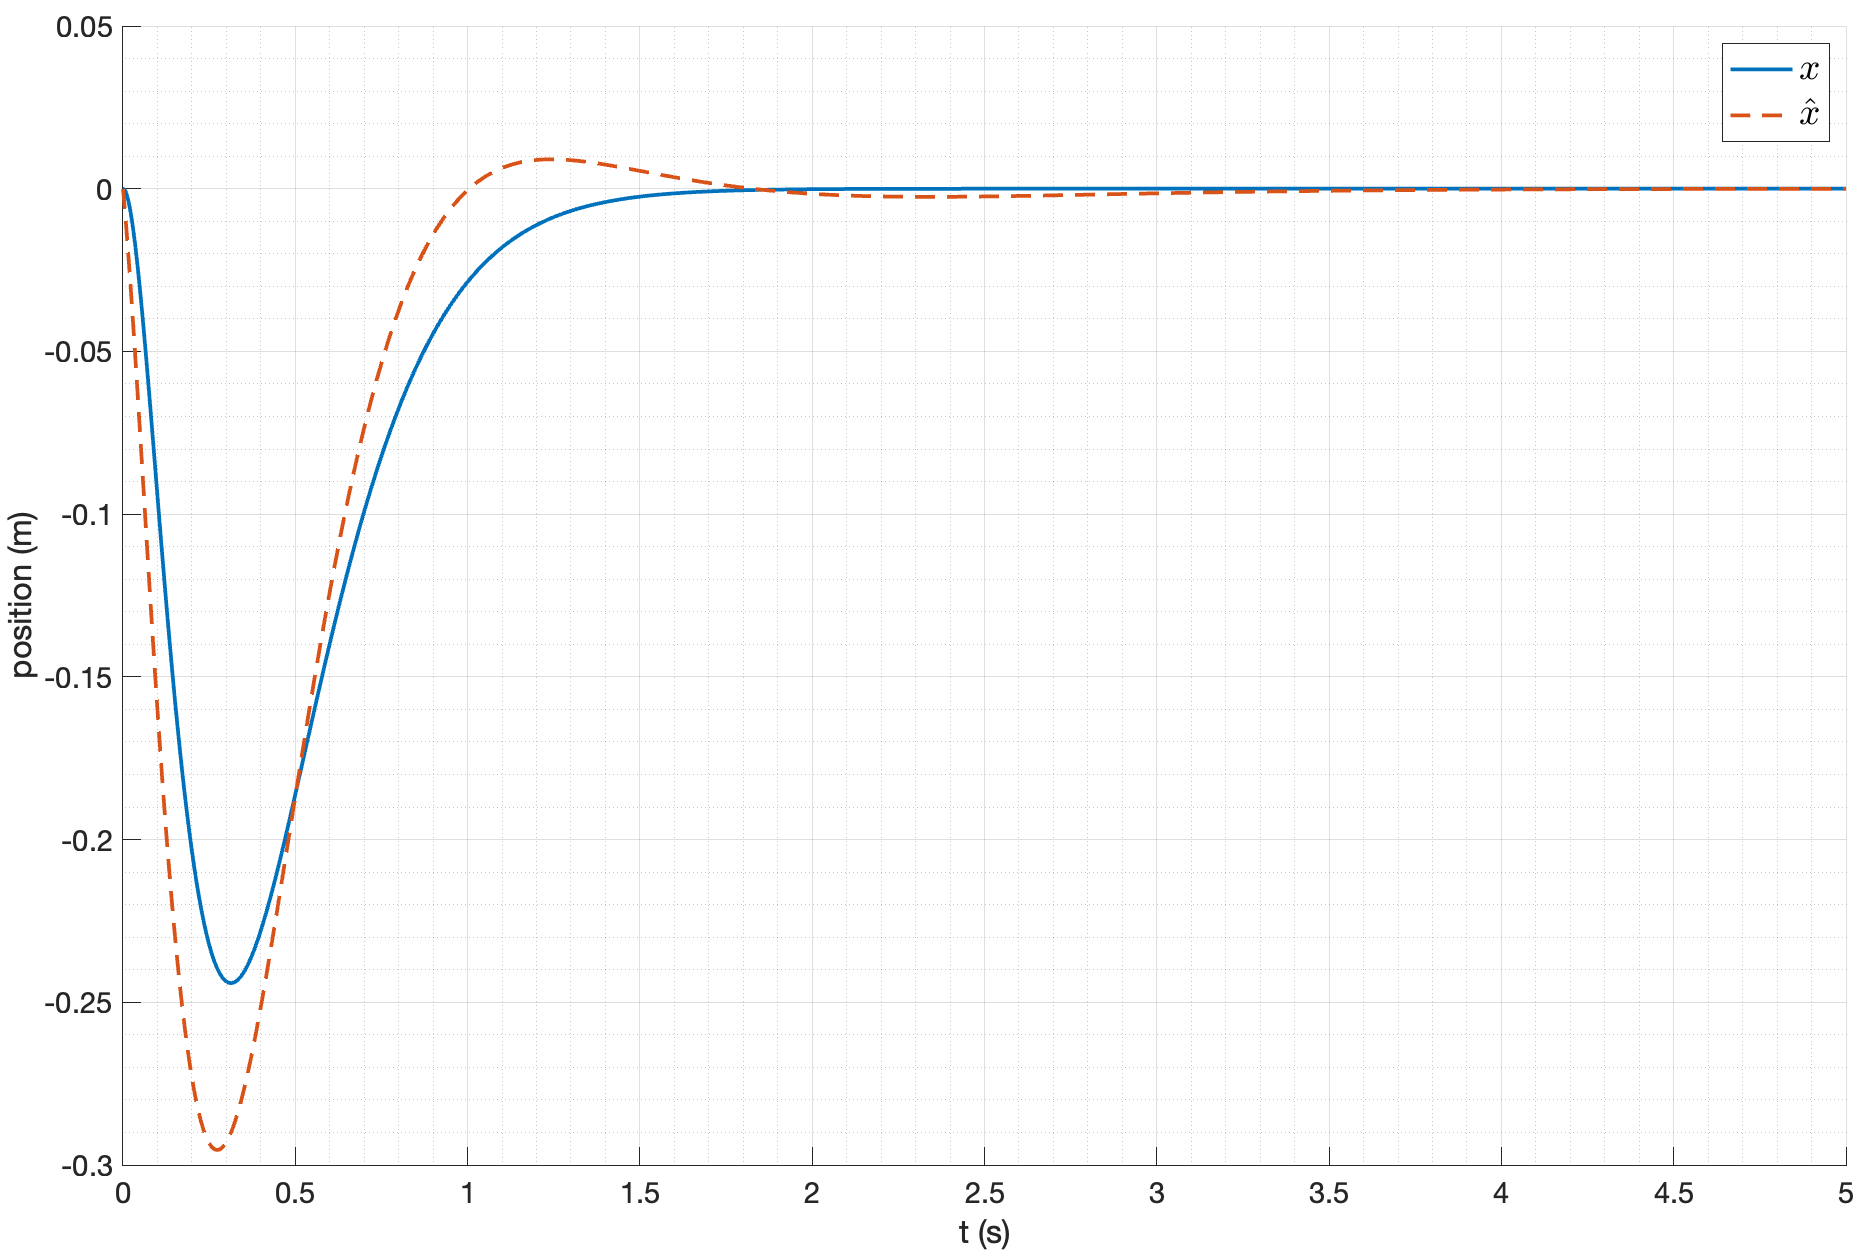
\includegraphics[width=\textwidth]{media/plots/modal_observer/observer_x_cmp_1.png}
        \caption{Оценка координаты тележки}
        \label{fig:observer_x_cmp_1}
    \end{subfigure}
    \begin{subfigure}[b]{0.45\textwidth}
        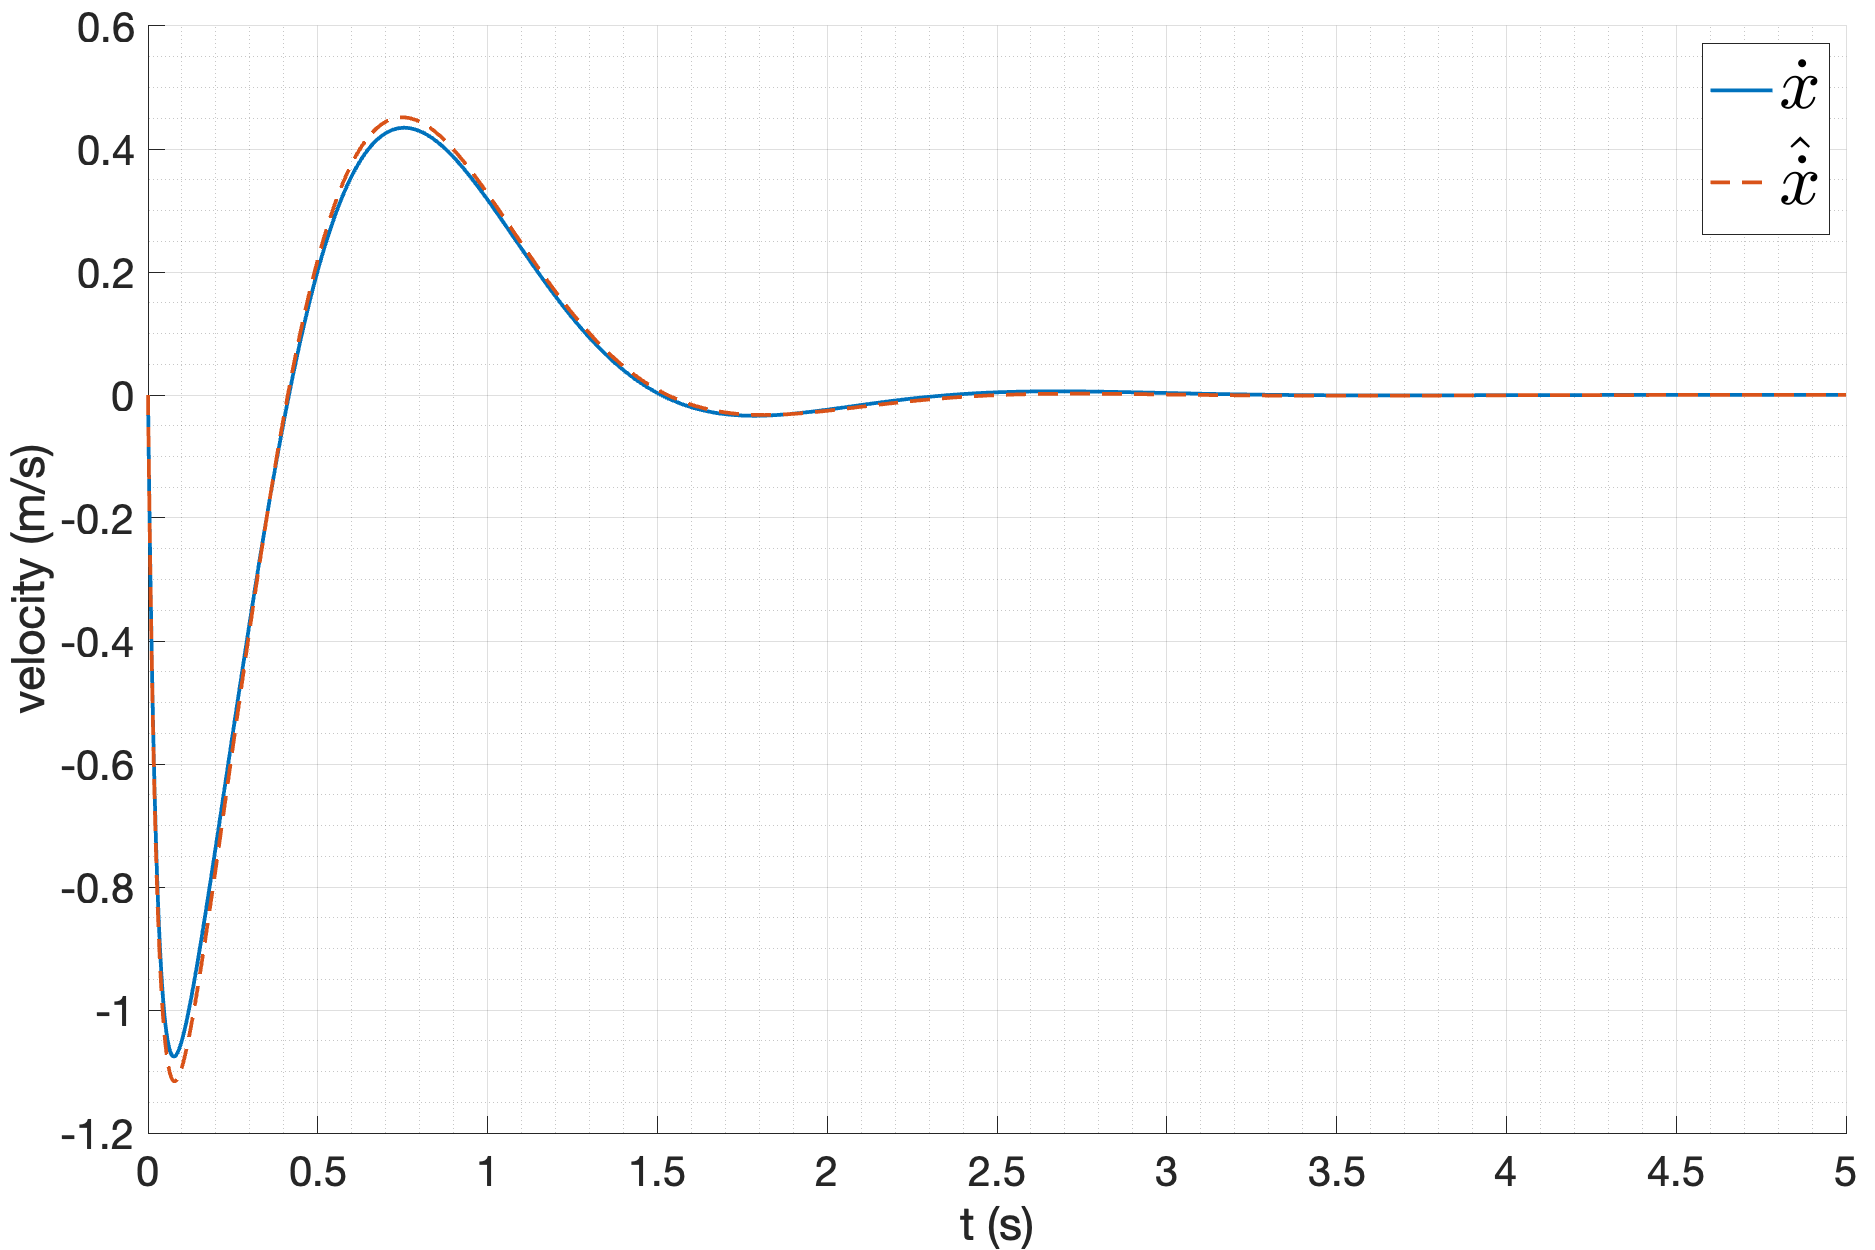
\includegraphics[width=\textwidth]{media/plots/modal_observer/observer_dotx_cmp_1.png}
        \caption{Оценка скорости тележки}
        \label{fig:observer_dotx_cmp_1}
    \end{subfigure}
    \begin{subfigure}[b]{0.45\textwidth}
        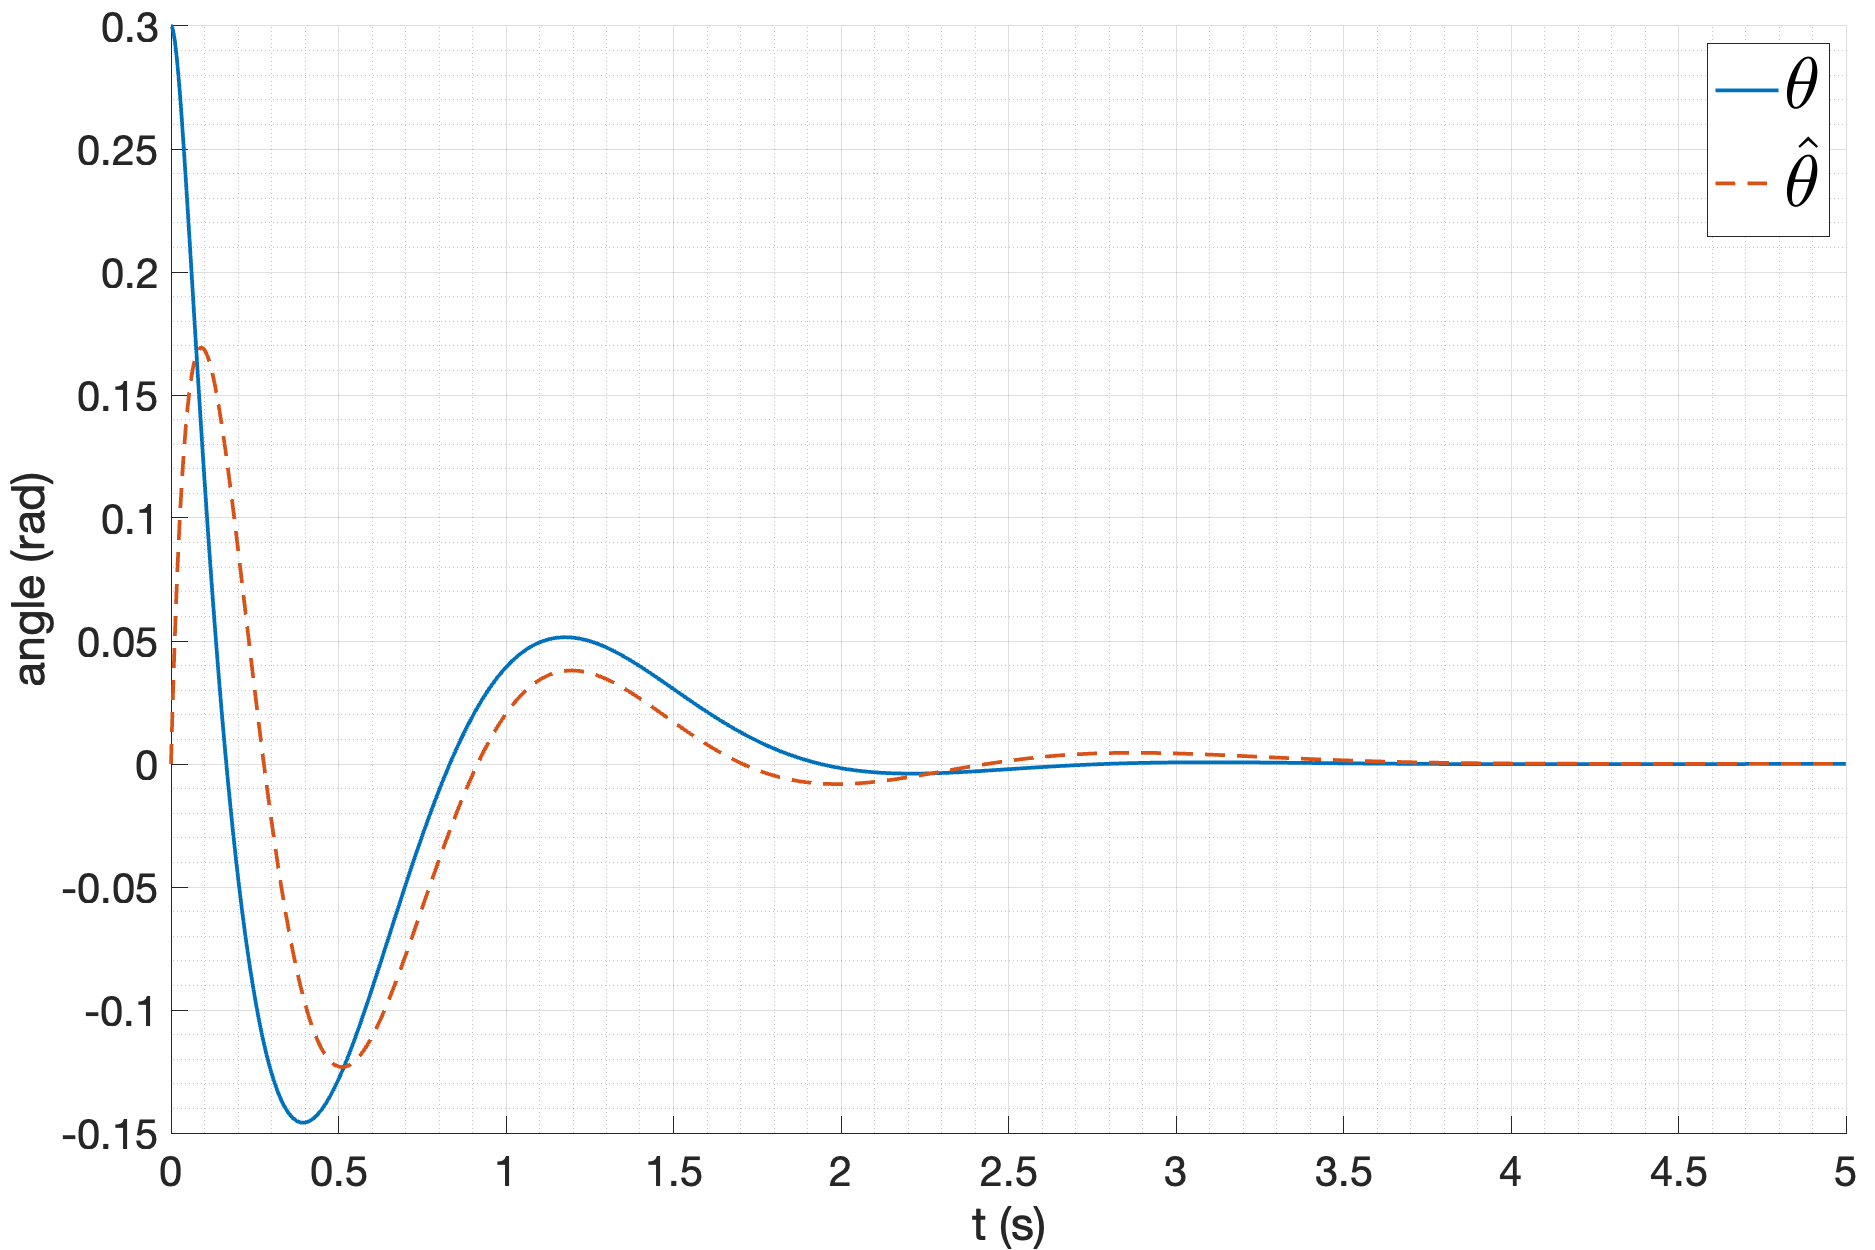
\includegraphics[width=\textwidth]{media/plots/modal_observer/observer_theta_cmp_1.png}
        \caption{Оценка угла отклонения маятника}
        \label{fig:observer_theta_cmp_1}
    \end{subfigure}
    \begin{subfigure}[b]{0.45\textwidth}
        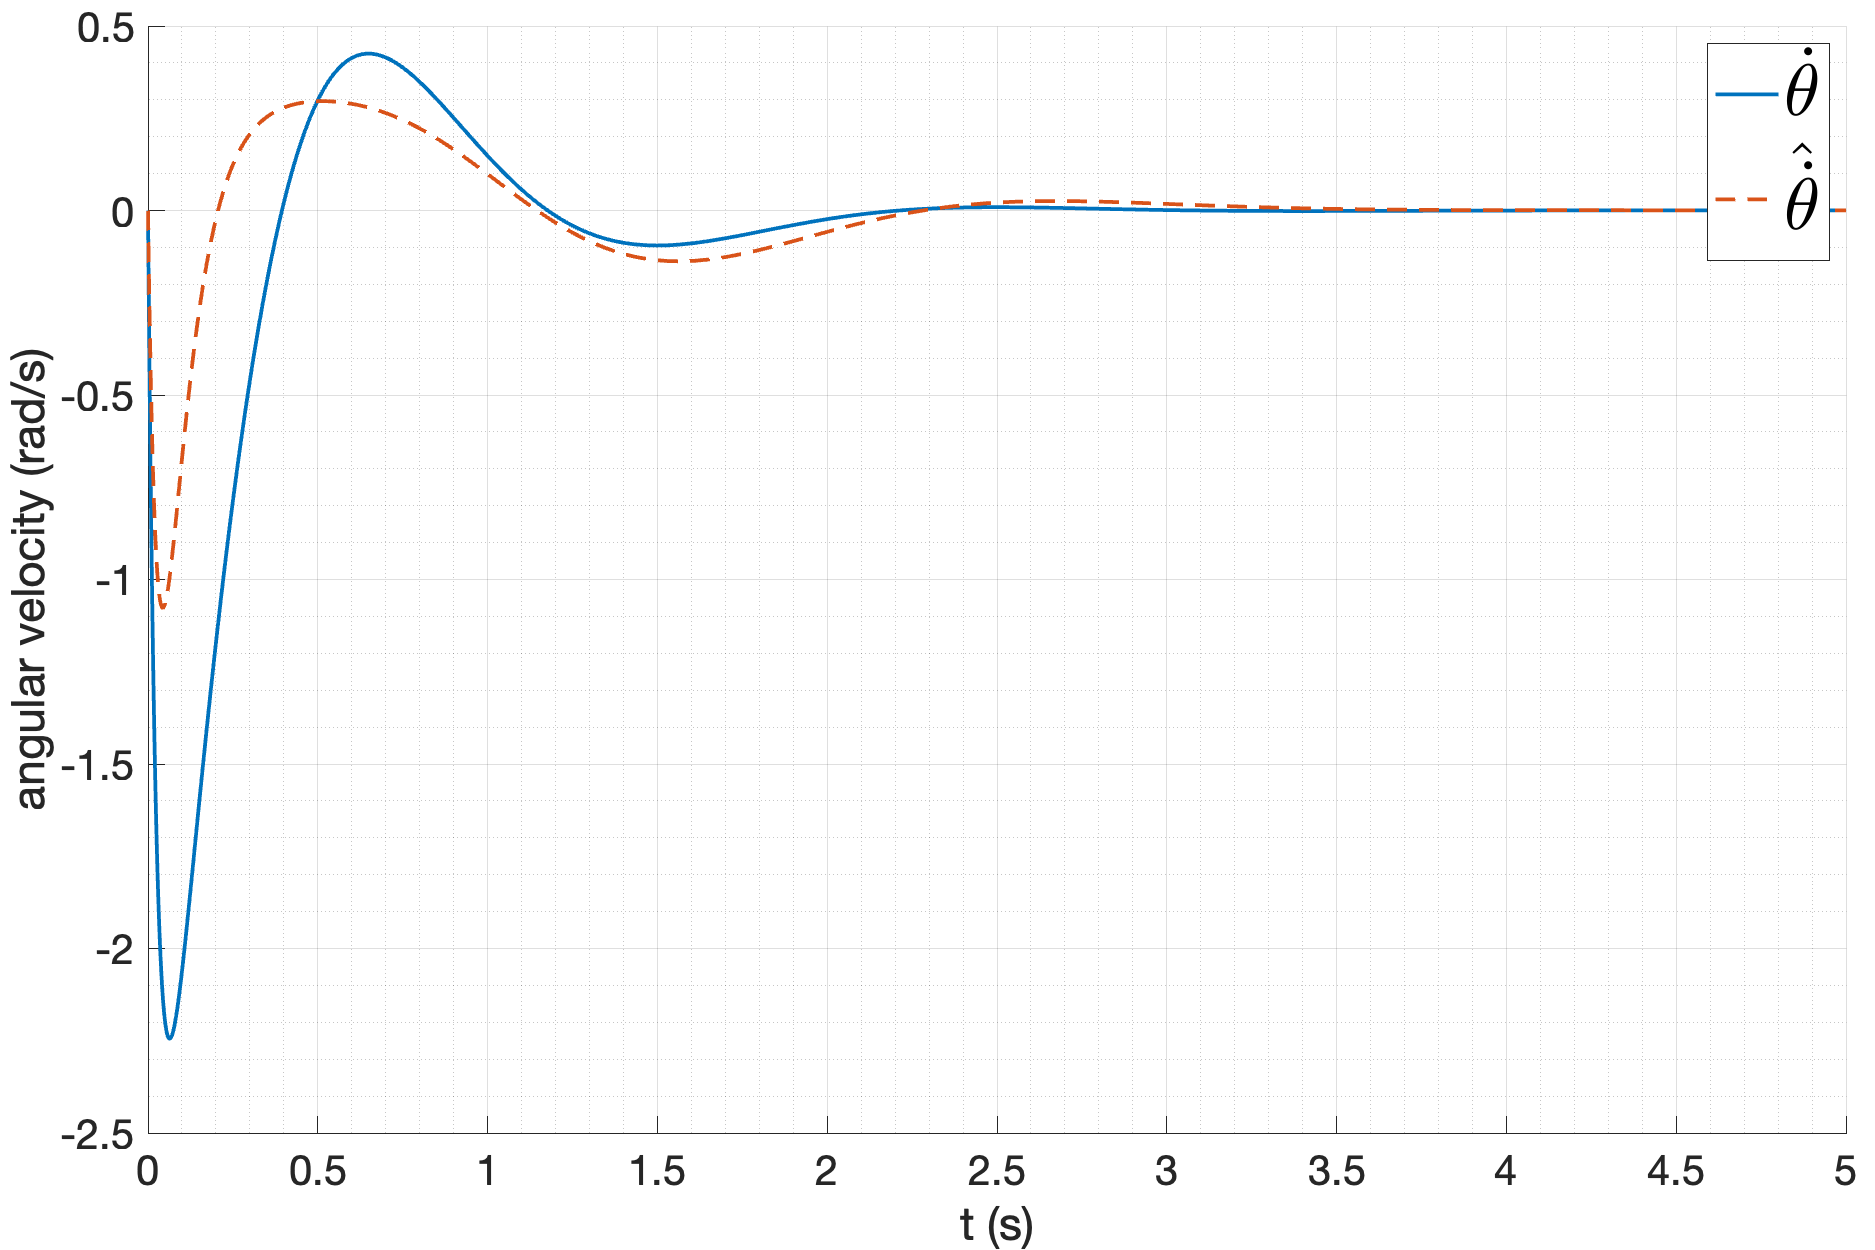
\includegraphics[width=\textwidth]{media/plots/modal_observer/observer_dottheta_cmp_1.png}
        \caption{Оценка угловой скорости маятника}
        \label{fig:observer_dottheta_cmp_1}
    \end{subfigure}
    \caption{Сравнение оценок состояния системы с реальным состоянием}
    \label{fig:observer_x_cmp_1_sep}
\end{figure}
\FloatBarrier
Можно увидеть, что оценка состояния нелинейной системы наблюдателем полного порядка
сходится к реальному состоянию системы, при этом время переходного процесса составляет около 2 секунд.
График ошибки оценки состояния системы приведен на рисунке \ref{fig:observer_err_1}.
\begin{figure}[ht!]
    \centering
    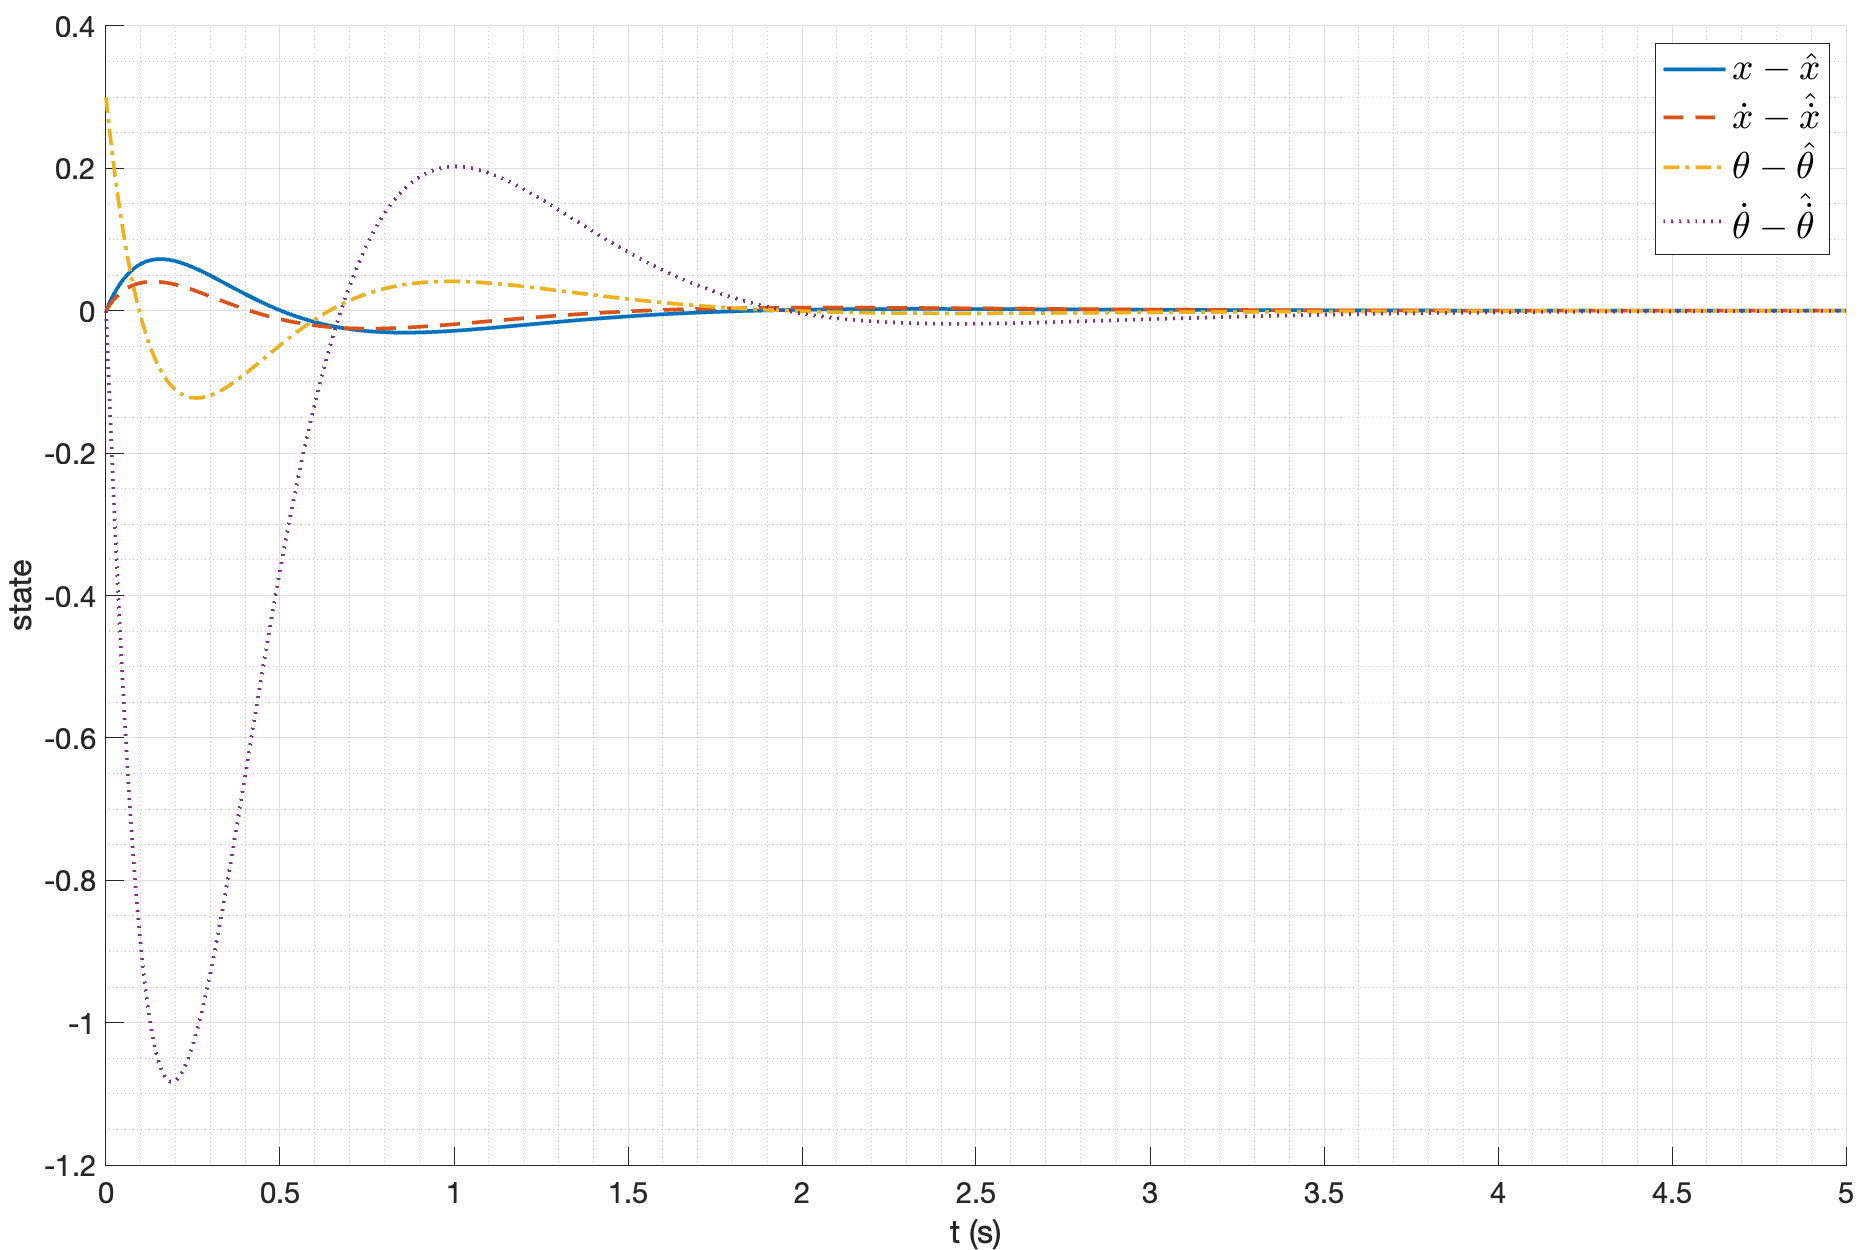
\includegraphics[width=\textwidth]{media/plots/modal_observer/observer_err_1.png}
    \caption{Ошибка оценки состояния системы наблюдателем полного порядка}
    \label{fig:observer_err_1}
\end{figure} 

Теперь посмотрим на работу наблюдателя полного порядка с более большим по модулю спектром, например, 
$\begin{bmatrix}-10 & -10 & -10 & -10\end{bmatrix}$. Результаты моделирования приведены на
рисунке \ref{fig:observer_x_2} и \ref{fig:observer_x_cmp_2_sep}. 
\begin{figure}[ht!]
    \centering
    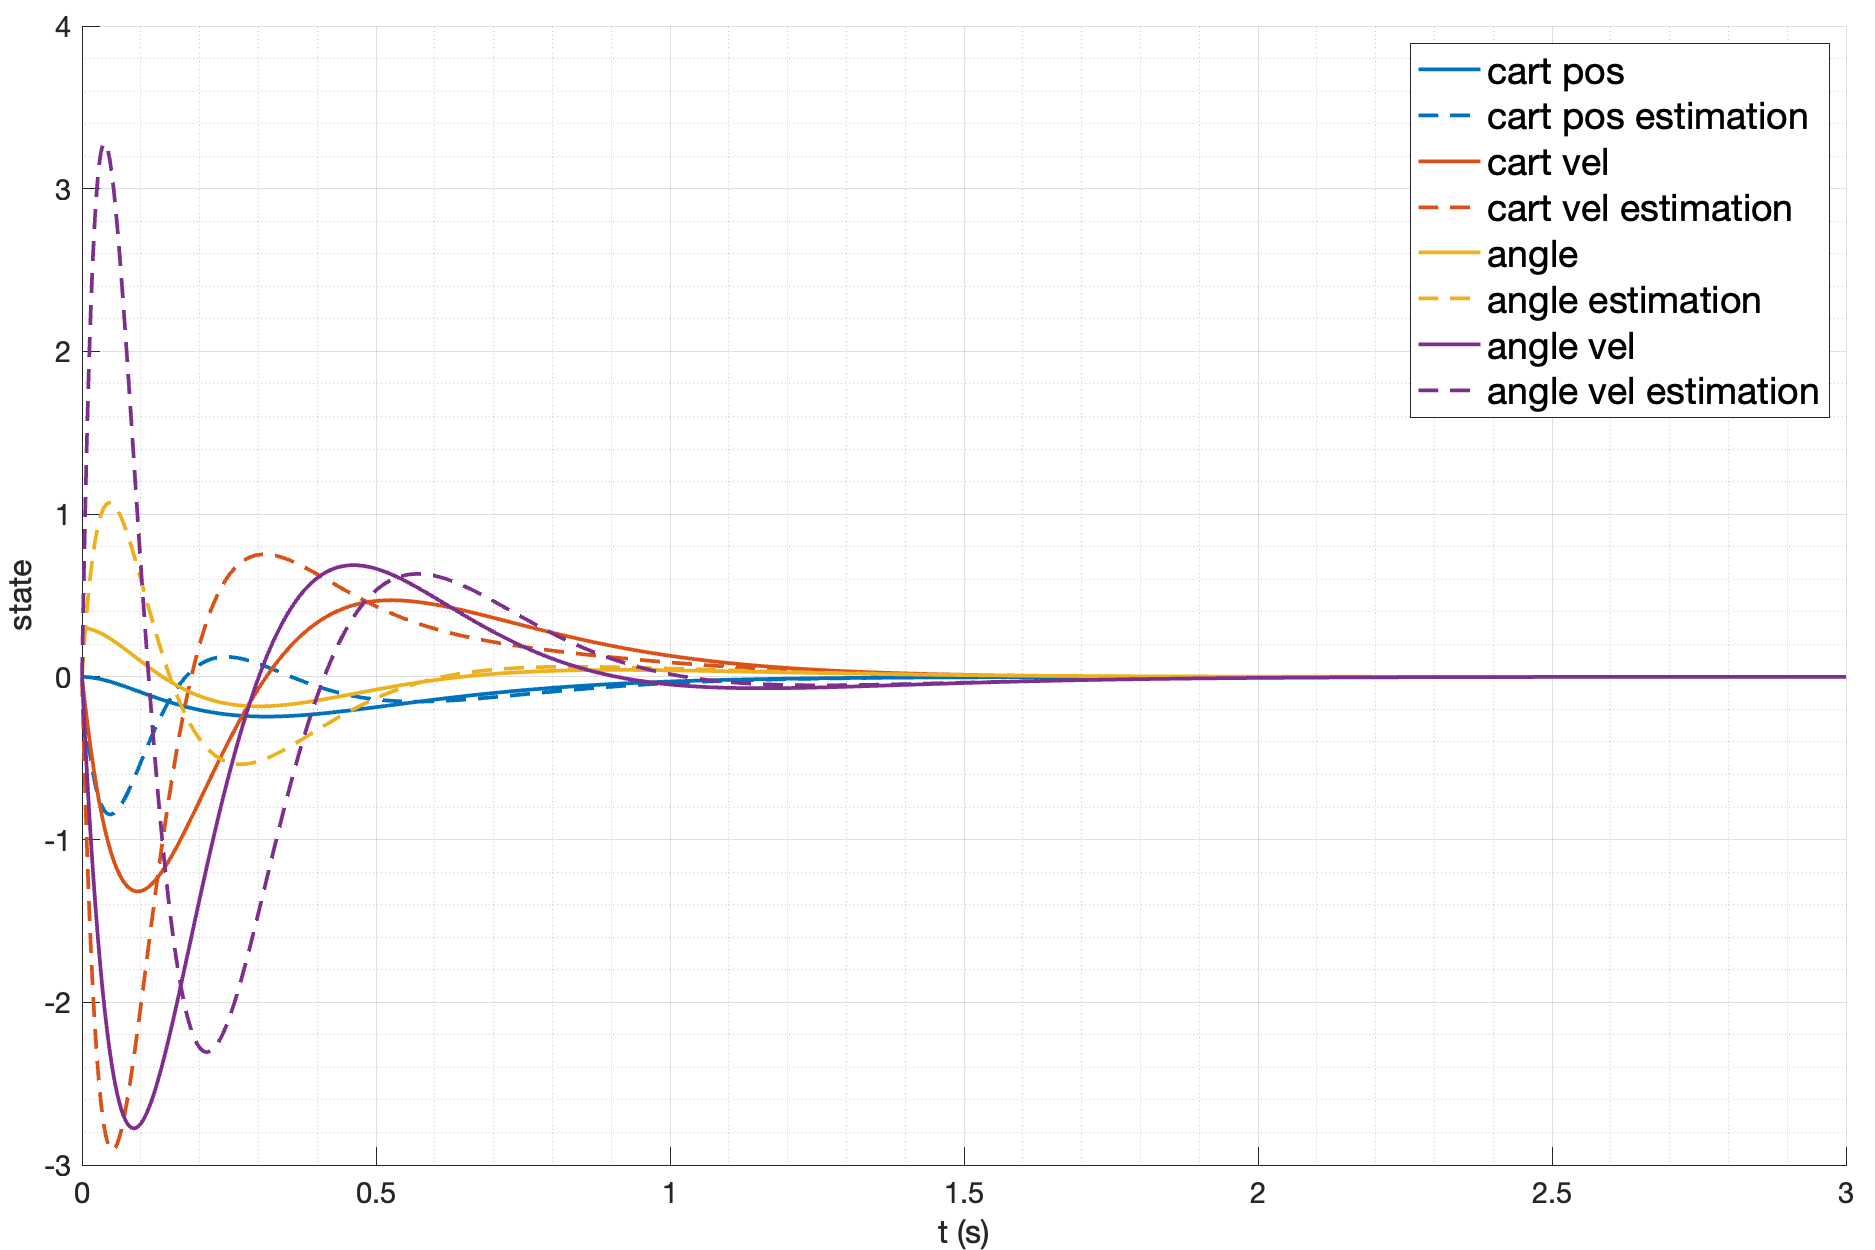
\includegraphics[width=\textwidth]{media/plots/modal_observer/observer_cmp_2.png}
    \caption{Результаты моделирования наблюдателя полного порядка}
    \label{fig:observer_x_2}
\end{figure}

\begin{figure}[ht!]
    \centering
    \begin{subfigure}[b]{0.45\textwidth}
        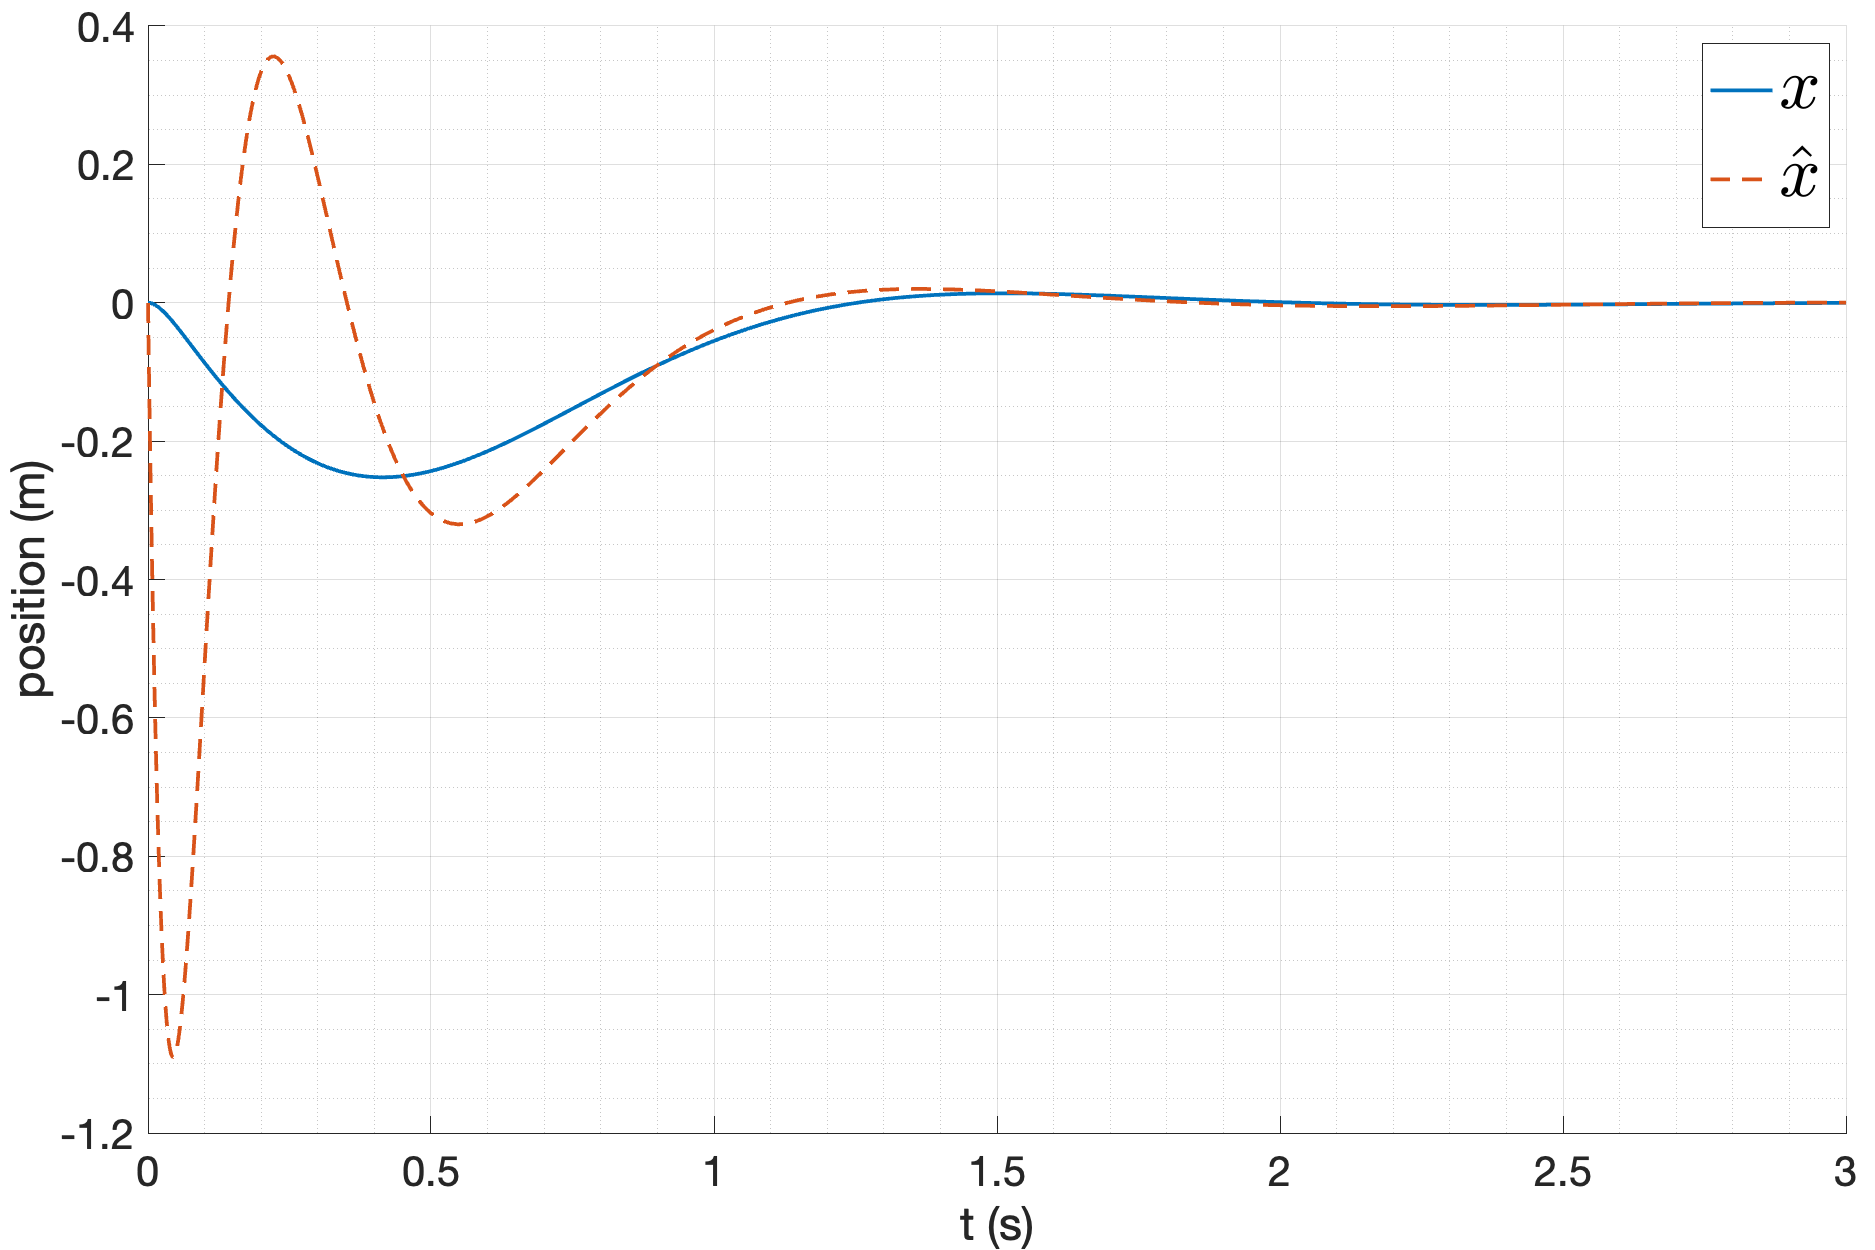
\includegraphics[width=\textwidth]{media/plots/modal_observer/observer_x_cmp_2.png}
        \caption{Оценка координаты тележки}
        \label{fig:observer_x_cmp_2}
    \end{subfigure}
    \begin{subfigure}[b]{0.45\textwidth}
        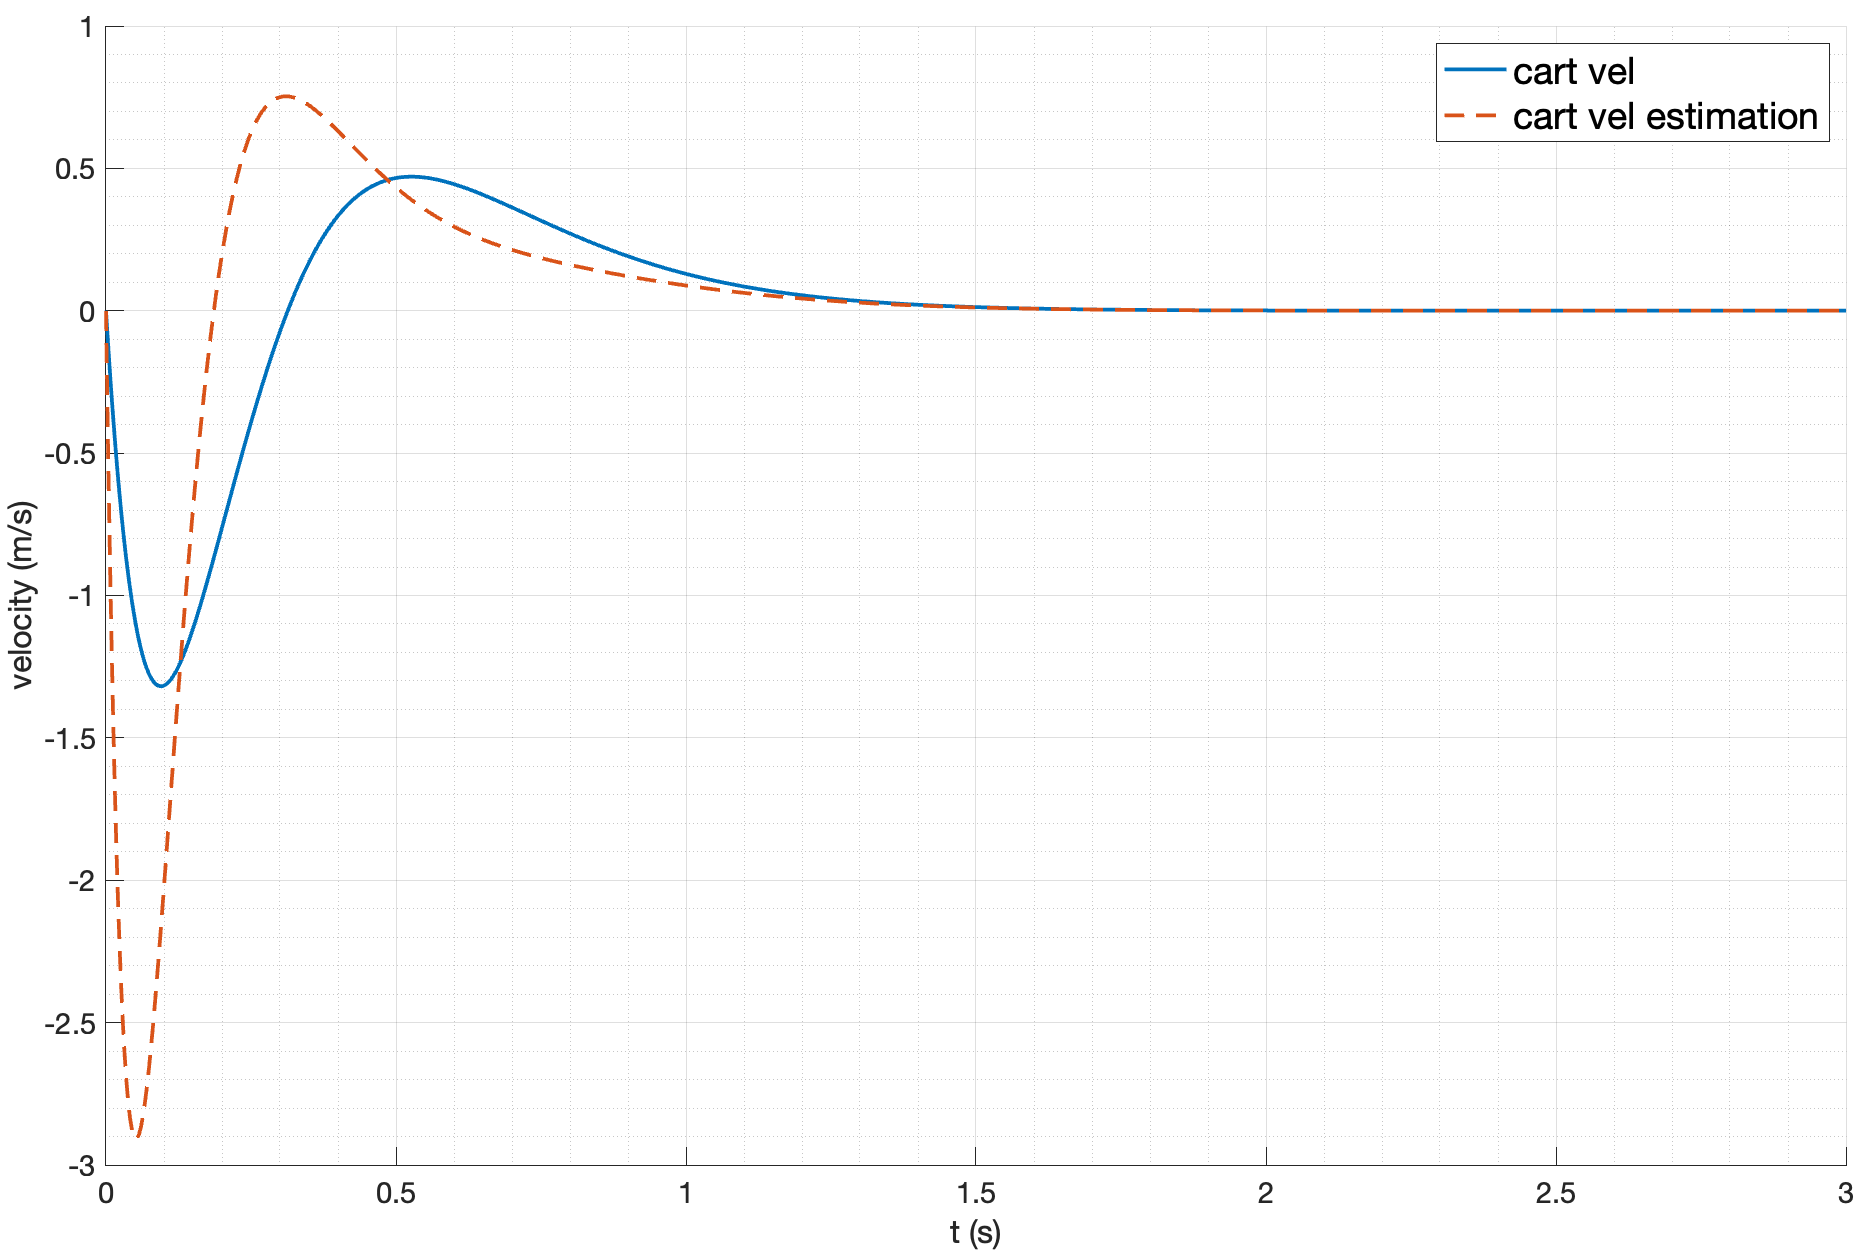
\includegraphics[width=\textwidth]{media/plots/modal_observer/observer_dotx_cmp_2.png}
        \caption{Оценка скорости тележки}
        \label{fig:observer_dotx_cmp_2}
    \end{subfigure}
    \begin{subfigure}[b]{0.45\textwidth}
        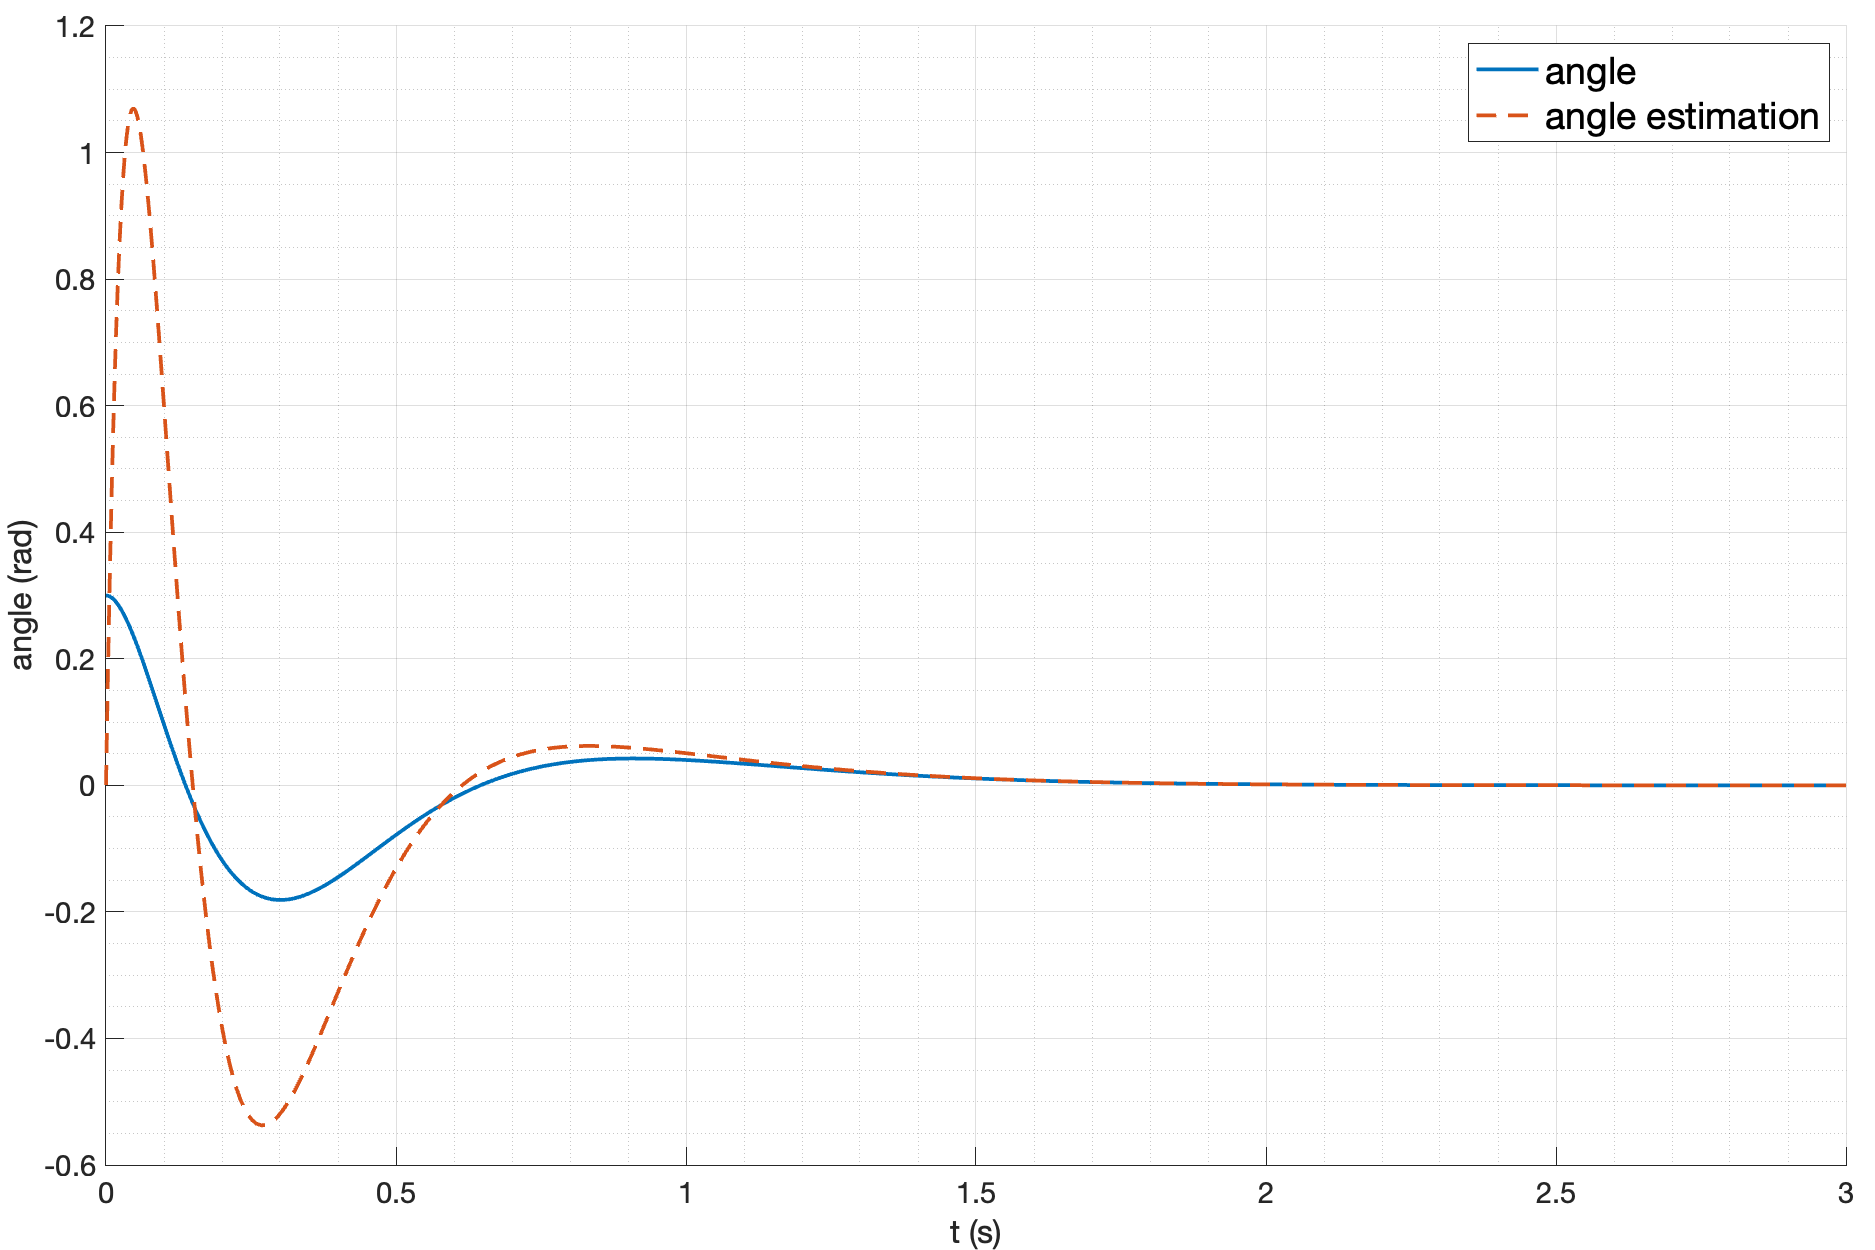
\includegraphics[width=\textwidth]{media/plots/modal_observer/observer_theta_cmp_2.png}
        \caption{Оценка угла отклонения маятника}
        \label{fig:observer_theta_cmp_2}
    \end{subfigure}
    \begin{subfigure}[b]{0.45\textwidth}
        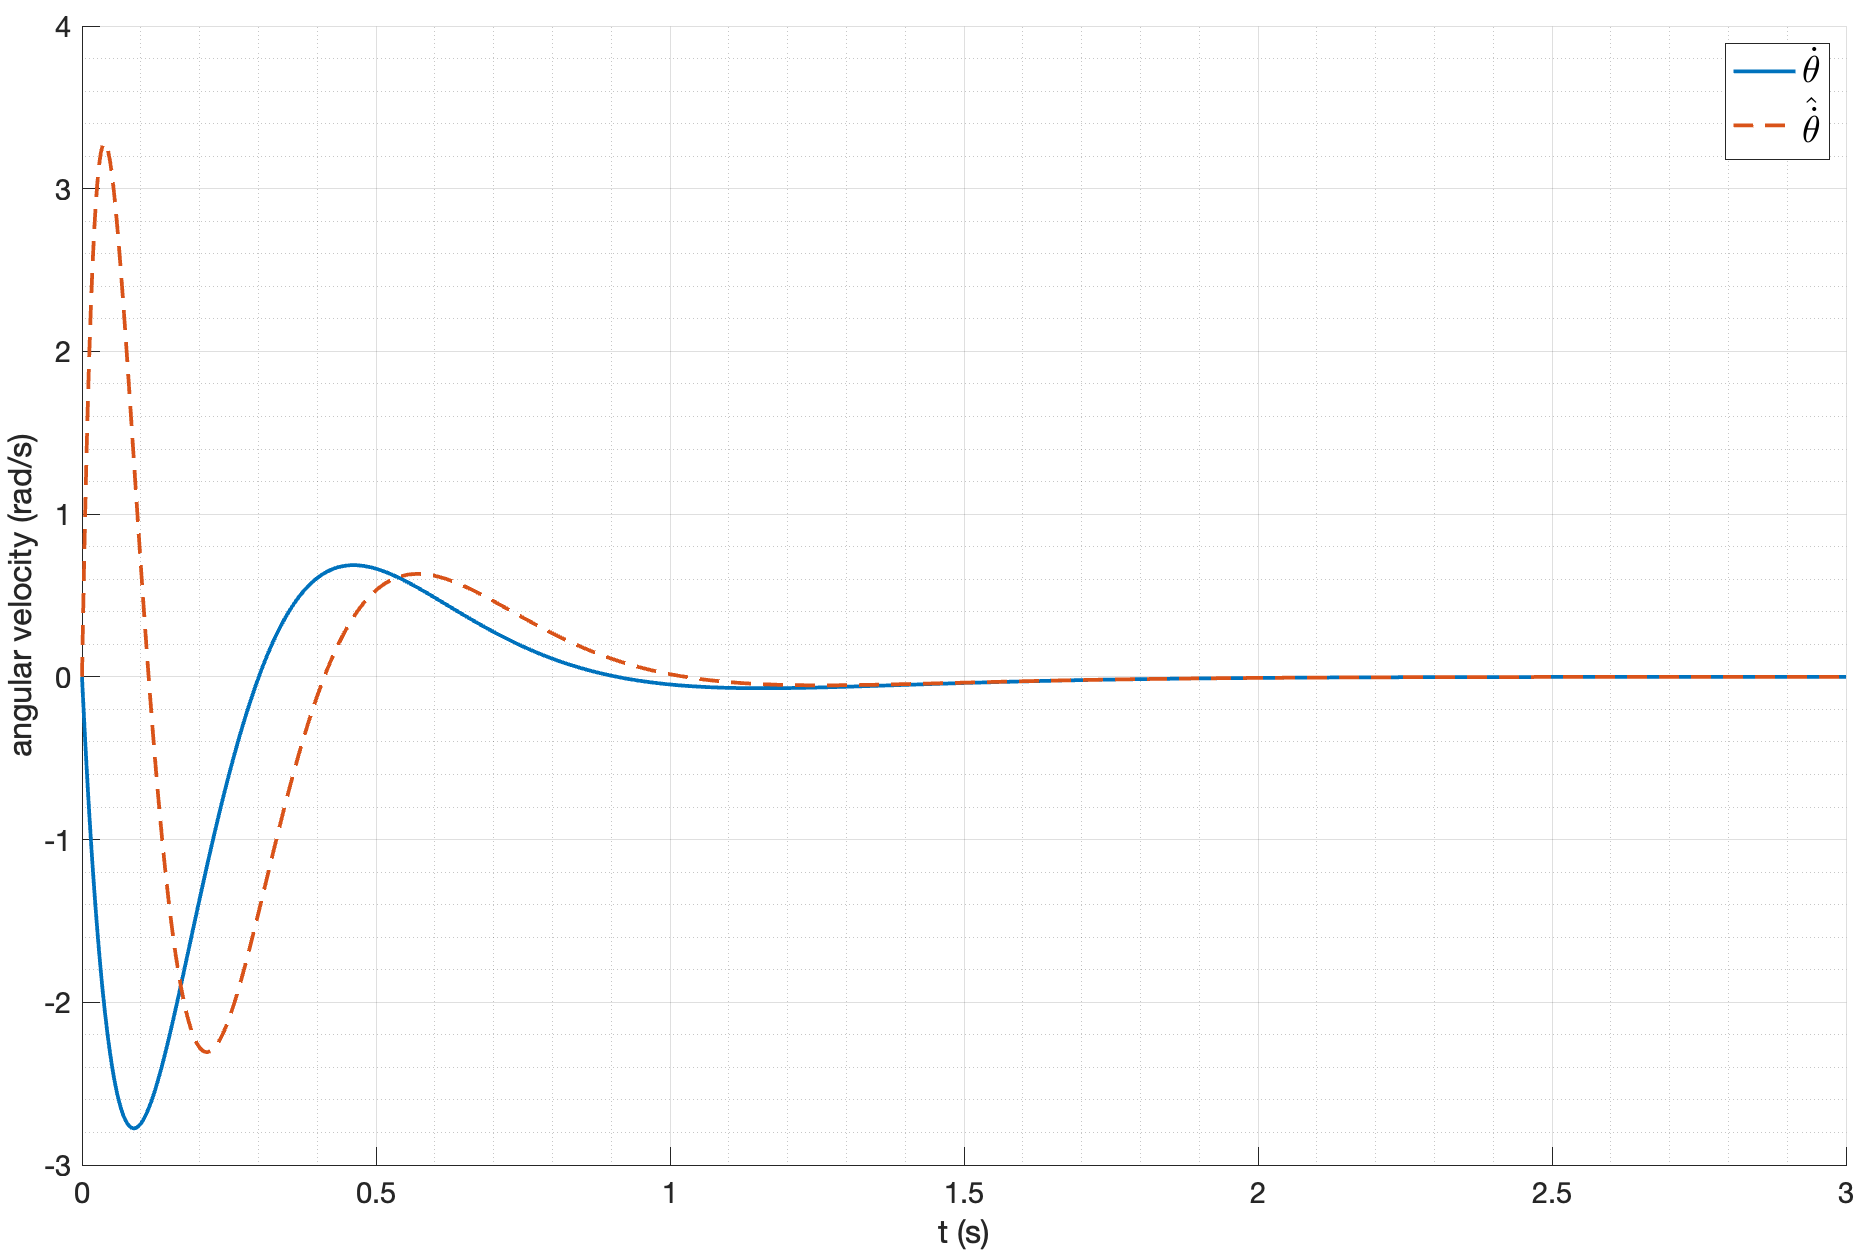
\includegraphics[width=\textwidth]{media/plots/modal_observer/observer_dottheta_cmp_2.png}
        \caption{Оценка угловой скорости маятника}
        \label{fig:observer_dottheta_cmp_2}
    \end{subfigure}
    \caption{Сравнение оценок состояния системы с реальным состоянием при $k = -10$}
    \label{fig:observer_x_cmp_2_sep}
\end{figure}
График ошибки оценки состояния системы приведен на рисунке \ref{fig:observer_err_2}.
\begin{figure}[ht!]
    \centering
    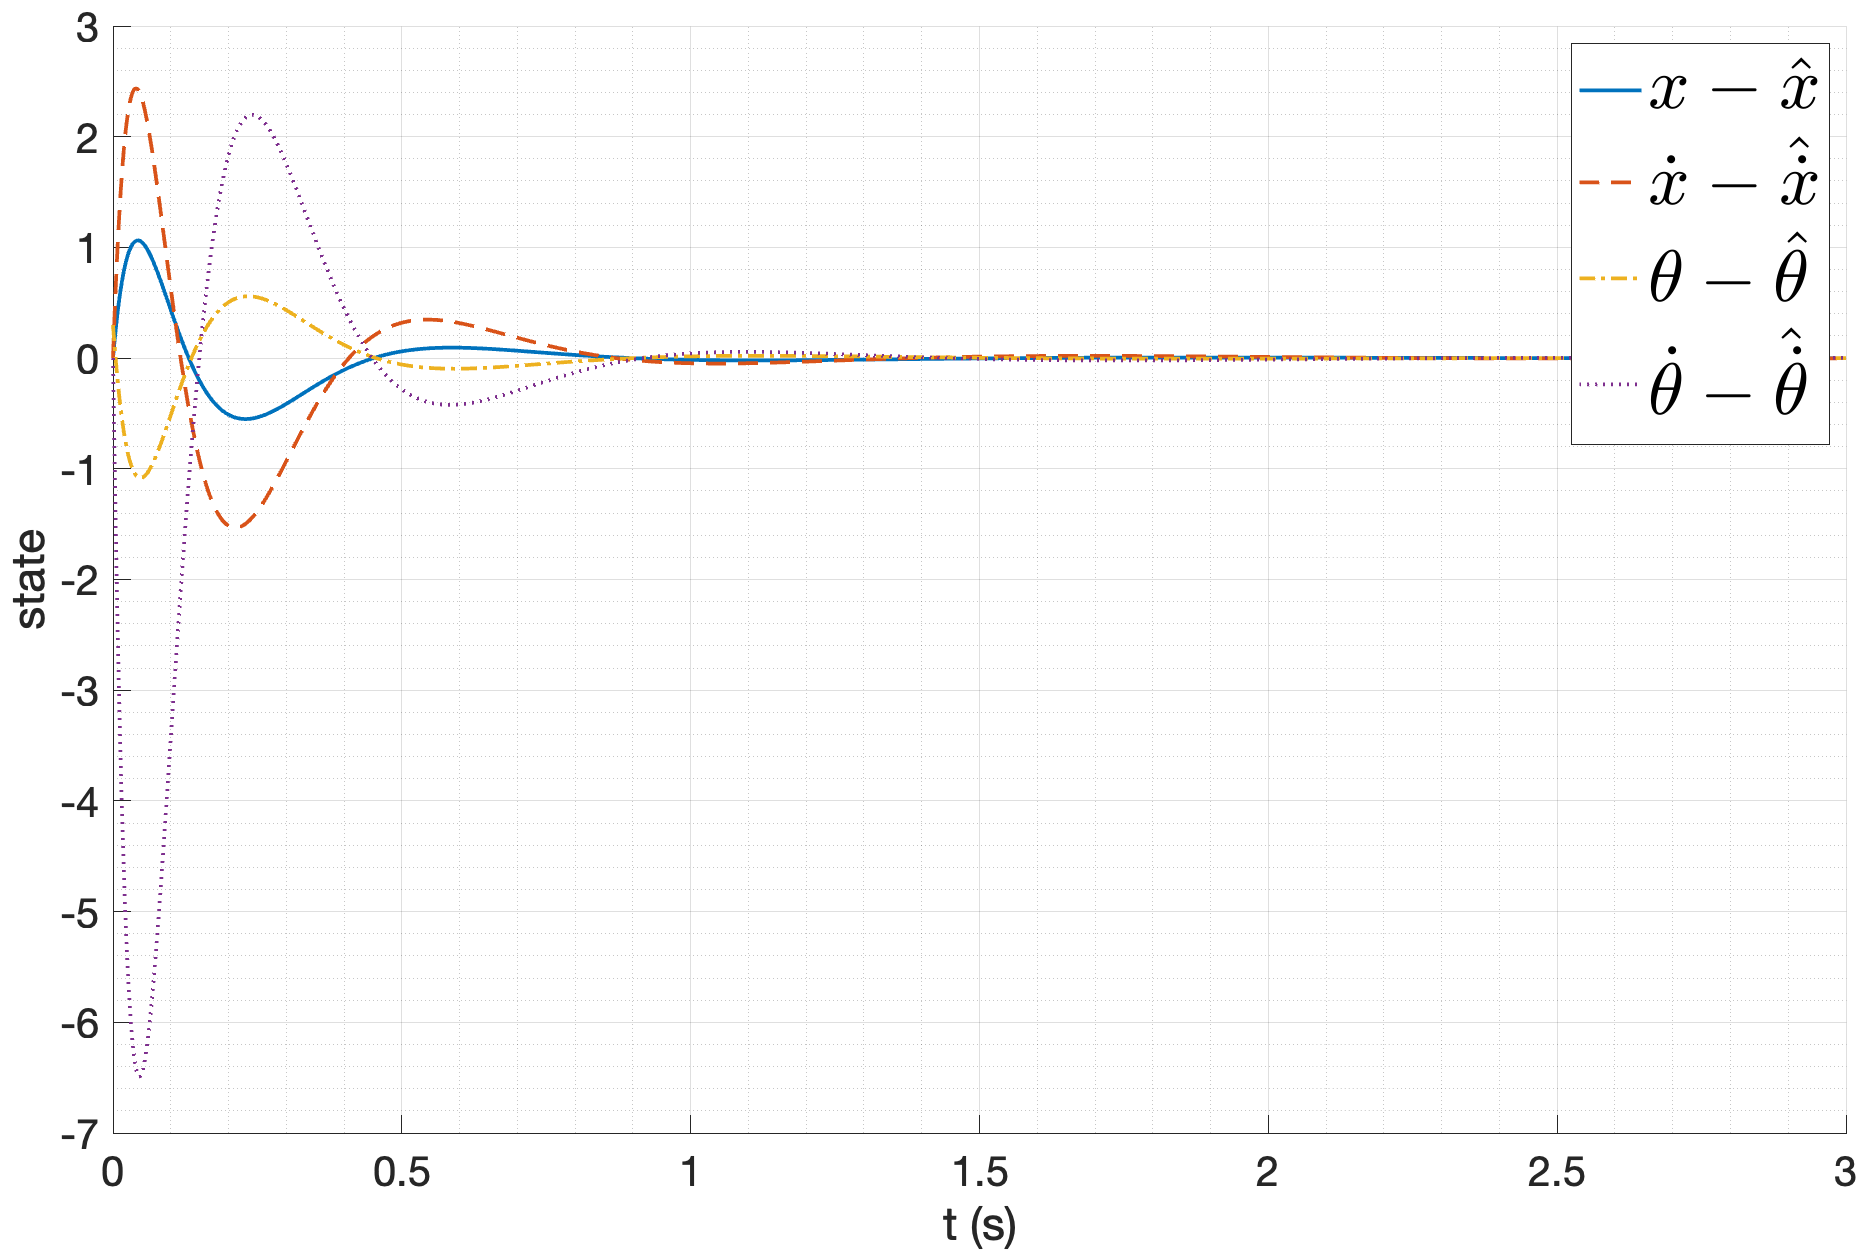
\includegraphics[width=\textwidth]{media/plots/modal_observer/observer_err_2.png}
    \caption{Ошибка оценки состояния системы наблюдателем полного порядка}
    \label{fig:observer_err_2}
\end{figure}
\FloatBarrier
Видно, что теперь время переходного процесса составляет около 1 секунды, что меньше, чем в случае 
наблюдателя с меньшими по модулю собственными числами. 

При этом можно заметить, что начальная ошибка оценки состояния системы увеличилась, особенно сильно это заметно
для оценки угловой скорости маятника. Это может негативно сказаться на работе регулятора, замкнутого по наблюдаемому состоянию.

% \subsection{Наблюдатель пониженного порядка}
% Рассмотрим наблюдатель пониженного порядка:
% \begin{equation}
%     \begin{array}{ll}
%         \dot{\hat{z}} = \Gamma\hat{z} - Yy + (QB + YD)u\\
%         \hat{x} = \begin{bmatrix}
%             C \\ Q
%         \end{bmatrix}^{-1} \times \begin{bmatrix}
%             y - Du \\ 
%             \hat{z}
%         \end{bmatrix}
%     \end{array}
% \end{equation}
% Зададим желаемый спектр наблюдателя пониженного порядка $\{-1, -2\}$.

% Тогда матрица $Q$ находится из решения уравнения Сильвестра: 
% \begin{equation}
%    \Gamma Q - QA = YC 
% \end{equation}
% где $\Gamma$ -- матрица с желаемыми собственными числами. 